% main.tex — Vitrine v5: Capture-Adaptive Video-to-3D-Scene Pipeline for UE 5.8
% Academic report compiled with pdflatex + bibtex (4-pass).
%
% House style inherited from report/main_v4.tex:
%   documentclass report, a4paper, 11pt
%   Packages: inputenc, fontenc, babel, microtype, geometry, lmodern, inconsolata,
%             xcolor, graphicx, tikz, booktabs, tabularx, longtable, array,
%             amsmath, amssymb, csquotes, enumitem, caption, hyperref, bookmark,
%             fancyhdr, listings, tcolorbox, titlesec
%   Colour macros: UoSRed, DreamLabAccent, DarkBg, MidGrey, LightGrey, CodeBg,
%                  SuccessGreen, WarningAmber, DangerRed
%   Custom environments: keyfinding, technote (and recommendation from v4)
%   L{} column type
%   lstlisting bash configuration
%
% Dr John O'Hare, DreamLab AI Consulting Ltd — June 2026

\documentclass[a4paper,11pt]{report}

\usepackage[utf8]{inputenc}
\usepackage[T1]{fontenc}
\usepackage[british]{babel}
\usepackage{microtype}
\usepackage[a4paper,top=28mm,bottom=28mm,inner=26mm,outer=24mm,headheight=22pt]{geometry}
\usepackage{lmodern}
\usepackage[dvipsnames,svgnames,x11names]{xcolor}

\definecolor{UoSRed}{HTML}{B71234}
\definecolor{DreamLabAccent}{HTML}{6366F1}
\definecolor{DarkBg}{HTML}{0F172A}
\definecolor{MidGrey}{HTML}{64748B}
\definecolor{LightGrey}{HTML}{F1F5F9}
\definecolor{CodeBg}{HTML}{1E293B}
\definecolor{SuccessGreen}{HTML}{15803D}
\definecolor{WarningAmber}{HTML}{B45309}
\definecolor{DangerRed}{HTML}{B91C1C}

\usepackage{graphicx}
\graphicspath{{v5/}{figures/}{figures/v2/}{figures/v3/}}
\usepackage{tikz}
\usetikzlibrary{calc,positioning,arrows.meta,shapes.geometric,backgrounds,fit}
\usepackage{booktabs}
\usepackage{tabularx}
\usepackage{longtable}
\usepackage{array}
\newcolumntype{L}[1]{>{\raggedright\arraybackslash}p{#1}}
\newcolumntype{C}[1]{>{\centering\arraybackslash}p{#1}}
\usepackage{amsmath,amssymb}
\usepackage{csquotes}
\usepackage{enumitem}
\setlist{nosep,leftmargin=*}
\usepackage{caption}
\captionsetup{font=small,labelfont={bf,color=UoSRed}}

\usepackage[colorlinks=true,linkcolor=UoSRed,citecolor=DreamLabAccent,urlcolor=DreamLabAccent,
  bookmarks=true,bookmarksnumbered=true,
  pdfauthor={Dr John O'Hare},
  pdftitle={Vitrine: A Capture-Adaptive Video-to-3D-Scene Pipeline for Unreal Engine 5.8},
  pdfsubject={3D Gaussian Splatting, Unreal Engine 5.8, Capture-Adaptive Pipeline, Game Assets}]{hyperref}
\usepackage{bookmark}
\usepackage{url}

\usepackage{fancyhdr}
\pagestyle{fancy}
\fancyhf{}
\fancyhead[L]{\small\textcolor{MidGrey}{\leftmark}}
\fancyfoot[R]{\small\textcolor{MidGrey}{\thepage}}
\fancyfoot[C]{\small\textcolor{MidGrey}{Vitrine v5, DreamLab AI Consulting Ltd}}
\renewcommand{\headrulewidth}{0.4pt}
\renewcommand{\footrulewidth}{0.2pt}
\renewcommand{\headrule}{\hbox to\headwidth{\color{UoSRed}\leaders\hrule height \headrulewidth\hfill}}

\usepackage{listings}
\lstset{basicstyle=\ttfamily\footnotesize,backgroundcolor=\color{LightGrey},frame=single,
  rulecolor=\color{MidGrey},breaklines=true,showstringspaces=false,tabsize=2,
  keywordstyle=\color{DreamLabAccent}\bfseries,commentstyle=\color{MidGrey}\itshape,
  stringstyle=\color{SuccessGreen},extendedchars=true,
  literate={---}{{---}}3 {--}{{--}}2 {->}{{$\rightarrow$}}2
    {checkmark}{{\checkmark}}1 {>=}{{$\geq$}}2 {<=}{{$\leq$}}2}
\lstdefinestyle{bash}{language=bash,
  morekeywords={docker,curl,python3,git,cmake,cargo,pytest,docker-compose},
  keywordstyle=\color{DreamLabAccent}\bfseries}

\usepackage[most]{tcolorbox}
\newtcolorbox{keyfinding}[1][]{enhanced,colback=UoSRed!5,colframe=UoSRed,fonttitle=\bfseries,
  title={Key Finding},left=5mm,boxrule=0.8pt,#1}
\newtcolorbox{recommendation}[1][]{enhanced,colback=DreamLabAccent!6,colframe=DreamLabAccent,
  fonttitle=\bfseries,title={Recommendation},left=5mm,boxrule=0.8pt,#1}
\newtcolorbox{technote}[1][]{enhanced,colback=LightGrey,colframe=MidGrey,fonttitle=\bfseries,
  title={Technical Note},left=5mm,boxrule=0.6pt,#1}

\usepackage{titlesec}
\titleformat{\chapter}[display]{\normalfont\huge\bfseries\color{DarkBg}}
  {\textcolor{UoSRed}{\chaptertitlename\ \thechapter}}{8pt}{\Huge}
\titlespacing*{\chapter}{0pt}{-18pt}{26pt}
\titleformat{\section}{\normalfont\Large\bfseries\color{DarkBg}}{\textcolor{UoSRed}{\thesection}}{1em}{}
\titleformat{\subsection}{\normalfont\large\bfseries\color{DarkBg}}{\textcolor{DreamLabAccent}{\thesubsection}}{1em}{}

% Convenience macros
\newcommand{\chip}[2]{\textcolor{#1}{\textbf{#2}}}
\newcommand{\code}[1]{\texttt{#1}}
\newcommand{\validated}{\chip{SuccessGreen}{validated}}
\newcommand{\inprogress}{\chip{WarningAmber}{in progress}}
\newcommand{\designed}{\chip{MidGrey}{designed}}
\newcommand{\wip}{\chip{WarningAmber}{in progress}}
\newcommand{\built}{\chip{SuccessGreen}{built}}

% natbib-compatible bibliography style
\usepackage[numbers,sort&compress]{natbib}

\begin{document}
\sloppy

% ───────────────────────── Title page ─────────────────────────
\begin{titlepage}
\begin{tikzpicture}[remember picture, overlay]
  \fill[DarkBg] (current page.south west) rectangle (current page.north east);
  \foreach \r in {2,3.2,4.4,5.6} {
    \draw[UoSRed, opacity=0.15, line width=0.6pt]
      ($(current page.north west) + (2.5,-3)$) circle (\r);}
  \foreach \i in {0,0.8,...,6.4} {
    \draw[DreamLabAccent, opacity=0.10, line width=0.5pt]
      ($(current page.south east) + (-\i-1, 0.5)$) -- ($(current page.south east) + (-0.5, \i+1)$);}
  \fill[UoSRed] ($(current page.west) + (0,2)$) rectangle ($(current page.east) + (0,2.08)$);
  \fill[DreamLabAccent] ($(current page.west) + (0,1.9)$) rectangle ($(current page.east) + (0,1.94)$);
  \node[anchor=north west, text=UoSRed, font=\footnotesize\sffamily\bfseries, text width=13cm]
    at ($(current page.north west) + (3,-2)$)
    {v5 ACADEMIC REPORT \textcolor{MidGrey}{|} DREAMLAB REFERENCE RUN VALIDATED};
  \node[anchor=west, text=white, font=\fontsize{40}{44}\selectfont\bfseries\sffamily, text width=15cm]
    at ($(current page.west) + (3,5.6)$) {Vitrine};
  \node[anchor=west, text=white, font=\fontsize{13}{17}\selectfont\sffamily, text width=14cm]
    at ($(current page.west) + (3,3.2)$)
    {A Capture-Adaptive Video-to-3D-Scene Pipeline\\for Unreal Engine~5.8};
  \node[anchor=west, text=MidGrey, font=\normalsize\sffamily, text width=13cm]
    at ($(current page.west) + (3,0.5)$)
    {video \textbullet\ COLMAP \textbullet\ 3D Gaussian Splatting \textbullet\ SAM3 \textbullet\ TRELLIS.2\\
     NanoGS \textbullet\ mesh \textbullet\ xatlas bake \textbullet\ FBX \textbullet\ UE\,5.8 game assets};
  \node[anchor=west, text=white, font=\sffamily, text width=10cm]
    at ($(current page.west) + (3,-2.2)$)
    {\textbf{Dr John O'Hare}\\[2pt] DreamLab AI Consulting Ltd\\[8pt]
     \textcolor{MidGrey}{Pairs with the upstream}\\[2pt] \textbf{LichtFeld Studio} reconstruction engine};
  \node[anchor=west, text=DreamLabAccent, font=\sffamily\bfseries]
    at ($(current page.west) + (3,-5.0)$) {June 2026};
  \node[anchor=south east, text=MidGrey, font=\tiny\sffamily]
    at ($(current page.south east) + (-3,1)$)
    {v5.0 \textcolor{MidGrey}{|} CAPTURE-ADAPTIVE PIPELINE \textbullet\ UE\,5.8 DELIVERY};
\end{tikzpicture}
\end{titlepage}

% ───────────────────────── Front matter ─────────────────────────
\pagenumbering{roman}

% ── Abstract ──────────────────────────────────────────────────────────────────
\chapter*{Abstract}
\addcontentsline{toc}{chapter}{Abstract}
\markboth{Abstract}{Abstract}

Vitrine is a \textbf{capture-adaptive} video-to-3D-scene pipeline that turns
hand-held walkthrough footage into structured, game-ready assets for
\textbf{Unreal Engine~5.8}.  Rather than applying a fixed reconstruction recipe
to every capture, Vitrine first \emph{diagnoses} each dataset on four
orthogonal axes --- sharpness, coverage, available hardware, and deliverable
format --- and then selects the combination of components whose benefit matches
the diagnosed bottleneck.  The key insight is that the best pipeline is a
function of the data, not a property of the system.

The pipeline is validated end-to-end on the \textbf{dreamlab reference capture}:
a 600-frame, 4K/30\,fps handheld walkthrough of a workshop/studio space,
reconstructed with COLMAP (600/600 frames registered) and trained to a
2.48M-Gaussian splat.  The validated dreamlab run produces: a real-Gaussian splat
room rendered in UE\,5.8 via the \textbf{NanoGS} plugin (MIT, recompiled for
UE\,5.8); three TRELLIS.2 textured object FBXs (chair, vacuum, toolbox) placed at
pre-computed real-world coordinates; and a comparative TSDF mesh branch.

A central empirical finding is \textbf{honest and negative}: the dreamlab room is
\emph{capture-limited}, not extractor-limited.  2DGS surface reconstruction
achieves planarity 69.7\% versus TSDF 72.0\% --- a $\Delta=2.3$ percentage-point
gap within measurement noise.  Neither exceeds the fair-room threshold; the binding
constraint is motion blur in the source footage (MUSIQ $\approx$31), and no mesh
extractor can raise that ceiling.  The room is therefore delivered as the
LichtFeld-native splat hero via NanoGS; the polygonal-mesh mandate is satisfied by
the TRELLIS.2 object FBXs.

Two further contributions are reported: a \textbf{directional sharpness gate}
(structure-tensor minor eigenvalue $\lambda_2$) that distinguishes directional
motion blur from isotropic softness and raises the bottom-quartile sharpness of
selected frames by 20--38\%; and a full hardware characterisation of
\textbf{ArtiFixer}~\cite{delutio2026_artifixer} on the NVIDIA RTX~6000~Ada
(48\,GB, sm\_89), showing that three targeted OOM fixes reduce peak VRAM from
out-of-memory to 45.5\,GB, enabling the 14B coverage-gap refiner to run on
Ada-generation hardware.

\tableofcontents
\listoffigures
\listoftables

% ───────────────────────── Main matter ─────────────────────────
\cleardoublepage
\pagenumbering{arabic}

% ====================================================================
\chapter{Introduction}
\label{chap:intro}

% ── Problem ──────────────────────────────────────────────────────────────────
\section{The Problem: Real Captures Fail in Different Ways}
\label{sec:intro:problem}

Photorealistic 3D reconstruction from hand-held video is a mature technology: the
combination of Structure-from-Motion (SfM), 3D Gaussian Splatting
(3DGS)~\cite{kerbl2023_3dgs}, and game-engine delivery is now within reach of any
operator with a modern smartphone and a GPU workstation.  The unsolved problem is
not the algorithm --- it is the \emph{mismatch between the algorithm's assumptions
and the real-world data it receives}.

Real captures fail in qualitatively different ways.  A handheld walkthrough at
walking pace fails due to \emph{motion blur}: the Gaussian field faithfully records
blurry observations, and no mesh extractor or training recipe can recover
sub-shutter-speed detail from pixels that were never resolved.  A tripod scan of a
large space fails due to \emph{coverage gaps}: the camera never reached certain
surfaces, Gaussians sprout as floaters in the unobserved void, and the mesh
contains holes.  A mobile-phone RGB-only capture fails differently from an
iPhone-LiDAR capture.  A project that demands Nanite-compatible collision meshes
fails differently from one that accepts a volumetric splat.

Any single fixed reconstruction recipe will be sub-optimal for most of these cases.
Optimising the pipeline for blur-limited footage (e.g.\ BAD-Gaussians
deblur~\cite{zhao2024_badgaussians}) adds wasted compute on a dense-but-sharp
capture.  Applying ArtiFixer~\cite{delutio2026_artifixer} to a blur-limited room is
similarly wasted: the model stays faithful to observed pixels and only fills
\emph{unobserved} regions; on a dense-but-blurry capture, there are no unobserved
regions to fill.

% ── Thesis ──────────────────────────────────────────────────────────────────
\section{The Capture-Adaptive Thesis}
\label{sec:intro:thesis}

Vitrine's answer is the \textbf{capture-adaptive thesis}: \emph{diagnose first,
then route}.  Every incoming capture is profiled on four independent axes before
any 3D computation begins:

\begin{description}
  \item[Sharpness] Is motion blur the dominant defect, or is the footage sharp?
    Measured by MUSIQ no-reference IQA~\cite{ke2021_musiq} and a full-resolution
    variance-of-Laplacian score via \texttt{pyiqa}~\cite{chen2022_pyiqa}.
  \item[Coverage] Are under-observed regions (holes, floaters) the dominant
    defect, or is the reconstruction dense?  Measured by a per-surface-point
    viewpoint-count occupancy probe.
  \item[Hardware] Does the capture include a depth sensor (iPhone LiDAR, event
    camera), or is it RGB-only?
  \item[Deliverable] Is a volumetric splat room representation sufficient, or does
    the project mandate a polygonal mesh (for collision, LOD, Nanite)?
\end{description}

\noindent A \emph{router} (Figure~\ref{fig:router}) evaluates these four axes
independently and assembles the appropriate configuration.  The four axes are
orthogonal: sharpness and coverage can each be good or bad independently, hardware
is a given, and the deliverable requirement is a project constraint.  The
router's decision space has $2^4 = 16$ nominal configurations; the section
files describe the validated subset.

% ── Contributions ─────────────────────────────────────────────────────────────
\section{Contributions}
\label{sec:intro:contributions}

This report documents the following validated contributions:

\begin{enumerate}
  \item \textbf{Capture-adaptive router} (\S\ref{sec:method:overview}).  A
    four-axis diagnosis-and-route mechanism that selects pipeline components based
    on the capture profile rather than a fixed recipe.

  \item \textbf{NanoGS splat-hero room in UE~5.8}
    (\S\ref{sec:results:nanogs}).  The LichtFeld-native 3DGS output is cleaned with
    SuperSplat and rendered as real Gaussians inside UE~5.8 via the NanoGS plugin,
    recompiled from its UE~5.6/5.7 codebase.  This closes the prior ``LiDAR
    point-cloud workaround'' and delivers the highest fidelity available from the
    captured data without an intermediate mesh-extraction step.

  \item \textbf{TRELLIS.2 object FBXs in UE~5.8}
    (\S\ref{sec:results:objects}).  Three dreamlab objects (chair, vacuum,
    toolbox) are reconstructed as textured polygonal game assets via the
    TRELLIS.2~\cite{xiang2025_trellis2} \texttt{hull\_e2e} workflow and placed at
    pre-computed real-world coordinates, satisfying the Nanite polygonal-mesh
    mandate without requiring the room to be meshed.

  \item \textbf{Empirical capture-limited finding}
    (\S\ref{sec:results:mesh}).  A controlled comparison of 2DGS and TSDF
    mesh extraction on the dreamlab capture establishes that the room is
    capture-limited: SOTA surface reconstruction provides no measurable benefit
    over a legacy TSDF on motion-blurred input.

  \item \textbf{Directional sharpness gate}
    (\S\ref{sec:results:framegate}).  An upgraded frame-quality gate based on the
    structure-tensor minor eigenvalue $\lambda_2$ that distinguishes
    directional motion blur from isotropic softness and raises the bottom-quartile
    sharpness of selected frames by 20--38\%.

  \item \textbf{ArtiFixer on Ada sm\_89}
    (\S\ref{sec:results:artifixer}).  Three targeted VRAM fixes reduce
    ArtiFixer~\cite{delutio2026_artifixer} peak usage from OOM to 45.5\,GB on a
    48\,GB RTX~6000~Ada, enabling the coverage-gap refiner to run on Ada-generation
    hardware without a FlashAttention-3 dependency.
\end{enumerate}

\begin{keyfinding}
The dreamlab reference run validates the capture-adaptive architecture on real data.
The headline lesson is honest: a SOTA mesh extractor cannot raise the quality ceiling
set by the source footage.  The splat-hero path (NanoGS) is both the highest-fidelity
and the most pipeline-lean option for a blur-limited capture; recapture at shorter
shutter speed is the real quality lever.
\end{keyfinding}

% ====================================================================
\chapter{Technologies and Related Work}
\label{chap:tech}

% sec_technologies.tex — Vitrine v5: Technologies and Related Work
% Capture-adaptive video→3D→UE 5.8 pipeline.
% Included by the v5 master document.
%
% British English throughout.
% All \cite{} keys are defined in report/v5/references.bib.

\section{Technologies and Related Work}
\label{sec:tech}

Vitrine assembles a heterogeneous stack that spans classical Structure-from-Motion
(SfM), neural radiance fields, volumetric 3D Gaussian representations, generative
diffusion models, and real-time game-engine delivery.  This section surveys each
component in pipeline order, placing Vitrine's choices in the context of the
relevant literature and explaining the motivation for each decision.

% ─────────────────────────────────────────────────────────────────────────────
\subsection{Scene Reconstruction: from Radiance Fields to Gaussians}
\label{sec:tech:recon}

\paragraph{Neural Radiance Fields.}
The modern era of photogrammetric reconstruction from uncontrolled video begins with
\emph{NeRF} \cite{mildenhall2020_nerf}, which encodes a scene as a continuous
volumetric function and synthesises novel views by differentiably integrating colour
and density along camera rays.  NeRF established the benchmark for view-synthesis
fidelity but requires minutes-to-hours of training per scene and cannot render in
real time.  Mip-NeRF~360 \cite{barron2022_mipnerf360} extended the approach to
unbounded outdoor scenes with anti-aliasing, but the fundamental throughput barrier
remained.

\paragraph{3D Gaussian Splatting.}
Kerbl~et~al.\ \cite{kerbl2023_3dgs} replaced the implicit MLP with an explicit set
of anisotropic 3D Gaussians, each carrying position, covariance, opacity, and
spherical-harmonic colour coefficients.  Differentiable tile-based rasterisation
renders the scene at real-time frame rates while achieving view-synthesis quality
competitive with the best NeRF variants on standard benchmarks.  The explicit,
editable representation and the absence of a ray-marching inner loop make 3DGS the
natural foundation for a practical pipeline.  Vitrine uses the
\emph{LichtFeld~Studio} \cite{lichtfeld2026} implementation, which adds
ImprovedGS\texttt{+} densification heuristics and a native C\texttt{++}23/CUDA
training loop exposed through a 70-tool MCP server.

A key limitation of 3DGS for game-engine delivery is its incompatibility with
standard rasterisation pipelines: Gaussians cannot be imported directly as
collision-ready meshes or LOD assets.  NanoGS \cite{nanogs2026}, released in March
2026, demonstrated a Nanite-inspired plugin for Unreal Engine~5 that applies
hierarchical LOD clustering and GPU-accelerated depth sorting to render splat point
clouds inside UE5 at interactive rates.  Vitrine uses NanoGS as an optional
``splat-in-UE'' path for scene preview, while polygonal meshes remain the primary
game-asset deliverable.

\paragraph{Structure from Motion and Feature Matching.}
Camera pose estimation is the prerequisite for all downstream reconstruction.
Vitrine uses COLMAP~\cite{schoenberger2016sfm, schoenberger2016mvs}, the de-facto
open-source SfM framework, for sparse reconstruction and multi-view stereo.  COLMAP
was historically paired with SIFT~\cite{lowe2004_sift} features; Vitrine replaces
SIFT with \emph{ALIKED}~\cite{zhao2023_aliked}, a lighter keypoint and descriptor
extractor built on a sparse deformable descriptor head that matches dense features
at a fraction of the memory cost.  Correspondence is established with
\emph{LightGlue}~\cite{lindenberger2023_lightglue}, an adaptive Graph Neural
Network matcher that prunes the attention graph based on estimated match difficulty,
achieving SuperGlue-level accuracy at substantially lower latency.  Together,
ALIKED+LightGlue represent the current state of the art in efficient
sparse matching and have been shown to improve downstream 3DGS quality on
challenging indoor captures.

% ─────────────────────────────────────────────────────────────────────────────
\subsection{Surface Meshing}
\label{sec:tech:meshing}

Gaussian splatting does not produce a mesh natively.  Vitrine requires polygonal
geometry for Unreal Engine collision, Nanite virtualisation, and UV-baked texture
export.  Several approaches have been proposed to bridge the gap.

\paragraph{Geometry-regularised Gaussian variants.}
\emph{SuGaR}~\cite{guedon2024_sugar} (Surface-aligned Gaussian splatting) adds a
regularisation term that encourages Gaussians to align with the scene surface,
enabling Poisson mesh extraction.  \emph{2DGS}~\cite{huang2024_2dgs} collapses 3D
Gaussians onto 2D oriented planar disks, recovering surface normals analytically and
facilitating TSDF-style marching-cubes extraction.  \emph{PGSR}~\cite{chen2024_pgsr}
(Planar-based Gaussian Splatting) pursues a similar idea in the TVCG setting,
representing local geometry via planar primitives regularised for planarity
consistency.  \emph{GOF}~\cite{yu2024_gof} (Gaussian Opacity Fields) derives a
volumetric opacity field from a ray-tracing formulation of Gaussian rendering,
enabling direct level-set mesh extraction via marching tetrahedra without Poisson
post-processing.

\paragraph{Post-hoc mesh extraction.}
\emph{MILo}~\cite{guedon2025_milo} (Mesh-In-the-Loop Gaussian Splatting) takes a
fundamentally different approach: it extracts a differentiable mesh at \emph{every
training iteration} and back-propagates mesh gradients into the Gaussian parameters,
enforcing bidirectional consistency between the volumetric and surface
representations.  Published as a SIGGRAPH Asia 2025 journal track paper (ACM TOG),
MILo produces the finest geometric detail of any extraction method tested on
Vitrine's captures and is used as the \emph{primary object-mesh backend}.

\emph{CoMe}~\cite{radl2026_come} (Confidence-based Mesh extraction) assigns a
learnable confidence value to each Gaussian, using it to balance photometric and
geometric supervision.  CoMe avoids the need for multi-view normal networks or
iterative extraction and runs substantially faster than MILo.  It serves as
Vitrine's \emph{primary scene-environment mesh backend}, with a TSDF fallback
(below) for scenes where CoMe confidence fails to converge.

\paragraph{TSDF fallback.}
Truncated Signed Distance Function fusion~\cite{curless1996_tsdf} with marching
cubes~\cite{lorensen1987_marching} integrated via \emph{Open3D}~\cite{zhou2018_open3d}
provides a geometry-agnostic fallback.  The \texttt{ScalableTSDFVolume} pipeline
integrates depth images rendered from the trained splat, producing watertight meshes
even for wide-baseline captures where Gaussian regularisation fails.  Vitrine uses
the legacy \texttt{ScalableTSDFVolume} path (rather than the newer VoxelBlockGrid)
for stability on large scenes.

% ─────────────────────────────────────────────────────────────────────────────
\subsection{Per-Object Reconstruction}
\label{sec:tech:objects}

Reconstructing individual objects to game-asset quality from a room-scale scan
requires segmentation, generalised-prior 3D generation, and texture synthesis.

\paragraph{Instance segmentation.}
Vitrine uses the \emph{Segment Anything Model}~(SAM)~\cite{kirillov2023_sam} and
its video-capable successor \emph{SAM~2}~\cite{ravi2024_sam2} for per-frame mask
propagation across the capture sequence.  SAM's promptable, class-agnostic
segmentation enables instance crops without domain-specific training.  The
\emph{SAM-3D~Objects} library~\cite{sam3dobjects2025} lifts SAM masks into 3D using
the reconstructed point cloud, providing per-object bounding volumes and concept
labels that drive downstream hull reconstruction.

\paragraph{Image-to-3D generation (primary path).}
\emph{TRELLIS.2}~\cite{xiang2025_trellis2} is the designated primary hull backend.
Developed at Tsinghua University and Microsoft Research and released under the MIT
Licence, TRELLIS.2 introduces O-Voxel (Omni-Voxel), a field-free sparse voxel
representation that encodes both geometry and physically-based rendering (PBR)
material attributes.  A 4B-parameter flow-matching model trained on diverse 3D asset
datasets generates fully textured meshes (base colour, metallic, roughness, opacity)
in 17--60\,s per object on an RTX~6000~Ada, and accepts up to 16 multi-view inputs,
directly consuming the image crops Vitrine provides.  It builds on the original
\emph{TRELLIS}~\cite{xiang2024_trellis} (CVPR~2025 Spotlight), which introduced the
SLAT (Structured Latent) representation for unified Gaussian/mesh/radiance-field
decoding.

\paragraph{Image-to-3D generation (secondary / hero-asset path).}
\emph{Hunyuan3D~2.0}~\cite{zhao2025_hunyuan3d20} and
\emph{Hunyuan3D~2.1}~\cite{hunyuan2025_21} from Tencent provide the highest
open-weight texture fidelity (up to 8K PBR), at the cost of higher latency
($\approx$139\,s per object).  The system comprises a shape-generation diffusion
transformer (Hunyuan3D-DiT) and a texture-synthesis model (Hunyuan3D-Paint),
separately invocable as ComfyUI nodes.  Vitrine uses Hunyuan3D-2.1 as the
secondary/hero-asset backend, activating it when an object is designated a focal
point of the scene.

\paragraph{Inpainting and view completion.}
Real captures invariably include occluded object faces that neither TRELLIS.2 nor
Hunyuan3D can hallucinate from the available views.  Vitrine uses two complementary
models.  \emph{FLUX.2-dev}~\cite{flux2025} (Black Forest Labs) is a 24B-parameter
rectified-flow transformer with a Mistral-3 text encoder, providing the strongest
available long-form prompt fidelity for rich appearance description.
\emph{Qwen-Image-Edit}~\cite{qwenvl2025} (Alibaba) is an instruction-following
visual-language model that uniquely supports instruction-driven view rotation, making
it the preferred recovery model for occluded-face completion and the only
commercially-licensed option in the stack.

\paragraph{View-generation conditioning.}
\emph{MV-Adapter}~\cite{mvadapter2024} (Apache-2.0) generates camera-conditioned
orbit sheets via ControlNet-compatible 6-view SDXL conditioning.  It provides a
lightweight, commercially-licensed alternative to non-commercial orbital-video
models for explicit camera-parametrised multi-view synthesis.

% ─────────────────────────────────────────────────────────────────────────────
\subsection{Reconstruction Enhancement: ArtiFixer}
\label{sec:tech:artifixer}

Even a dense splat contains structurally unobserved regions --- surfaces the camera
never approached --- where 3DGS places floaters, ghosts, or holes.  These defects
propagate into the downstream mesh and UE asset.
\emph{ArtiFixer}~\cite{delutio2026_artifixer}, from the NVIDIA Spatial Intelligence
Lab and presented at SIGGRAPH~2026, is an auto-regressive video-diffusion refiner
built on \emph{Wan2.1-T2V-14B}~\cite{wan2025}.  Its opacity-mixing trick
($z_{\mathrm{mix}} = O_z \cdot z_{\mathrm{deg}} + (1-O_z) \cdot \varepsilon$)
leaves observed pixels ($O_z \approx 1$) faithful to the input, while generating
freely in unobserved regions ($O_z \approx 0$) using a strong video-diffusion prior.
The \emph{ArtiFixer3D} variant distils the generated views back into an explicit
3DGRUT~\cite{wu2025_3dgut} Gaussian recon --- a cleaner splat whose downstream mesh
is measurably less noisy than the raw LichtFeld output on coverage-limited captures.

Vitrine forks ArtiFixer to run on RTX~6000~Ada (\texttt{sm\_89}) by replacing the
FlashAttention-3/4 build block with cuDNN SDPA, with no application-code changes
(ADR-020; see \S\ref{sec:method:overview}).  The enhanced recon branch is
\emph{optional and per-scene gated}: it activates only when a quality classifier
predicts coverage-limited rather than blur-limited failure, because ArtiFixer does
not deblur --- it stays faithful ($O_z \approx 1$) in observed-but-blurry regions.

% ─────────────────────────────────────────────────────────────────────────────
\subsection{Capture Quality and Frame Selection}
\label{sec:tech:quality}

The dominant quality bottleneck in real-world captures is motion blur, not
reconstruction arithmetic.  Vitrine addresses this at the frame-selection stage
before any 3D optimisation begins.

\paragraph{No-reference image quality.}
\emph{MUSIQ}~\cite{ke2021_musiq} (Multi-scale Image Quality Transformer) is a
patch-based transformer that processes full-size images at their native resolution,
using a hash-based 2D spatial embedding and scale embedding to capture image quality
at multiple granularities without fixed-size preprocessing distortion.  Trained on
PaQ-2-PiQ, KonIQ-10k, and SPAQ, MUSIQ achieves state-of-the-art no-reference image
quality assessment (NR-IQA) and is used as Vitrine's per-frame quality gate.
\emph{Q-Align}~\cite{wang2023_qalign} provides an LMM-based alternative that
emulates discrete human rating levels; it is evaluated as a higher-cost option
for batch scoring.  Both are accessed through \emph{pyiqa}~\cite{chen2022_pyiqa},
an open-source PyTorch IQA toolbox.

\paragraph{Focus and sharpness.}
Low-level sharpness is measured with the variance-of-Laplacian operator, a classical
focus measure that computes the variance of the Laplacian-filtered image; high
variance corresponds to sharp edges.  Pertuz~et~al.\ \cite{pertuz2013_focus}
provide a comprehensive survey and comparison of such operators.  The
full-resolution variant (applied on the full 4K frame rather than a downsampled
proxy) is used, as Vitrine's capture experiments showed that downsampling to 960p
compresses the dynamic range of the sharpness score by a factor of~105, masking
meaningful differences between frames.

\paragraph{Deblur-aware Gaussian training.}
When the frame-quality gate accepts footage that is mildly blurry rather than
sharply filtered, \emph{BAD-Gaussians}~\cite{zhao2024_badgaussians} (Bundle
Adjusted Deblur Gaussian Splatting, ECCV~2024) provides a training-time deblur
path.  BAD-Gaussians models the camera trajectory during exposure as a sequence of
virtual sharp cameras, blending their renders to simulate blur formation, and
jointly optimises the trajectory and the Gaussian parameters.  This yields both a
deblurred splat and corrected camera poses.

% ─────────────────────────────────────────────────────────────────────────────
\subsection{Texture Baking and Mesh Post-processing}
\label{sec:tech:texture}

Once a mesh is available from CoMe, MILo, or TSDF, Vitrine prepares it for
game-engine import.

\paragraph{UV atlas generation.}
Vitrine uses \emph{xatlas}~\cite{xatlas2018} for automatic UV atlas generation.
xatlas is a lightweight C\texttt{++}11 mesh-parameterisation library derived from
Thekla Atlas that segments meshes into charts, parameterises each chart, and packs
them into one or more non-overlapping atlases suitable for texture baking and
lightmap generation.

\paragraph{Texture baking.}
Vertex colours from the trained Gaussian splat are baked into UV-parametrised
textures using Blender's~\cite{blender2024} Cycles GPU renderer via the
\texttt{texture\_baker.bake\_from\_vertex\_colors} pipeline with \texttt{smooth=0}
(MeshCleaner smoothing disabled to preserve sharp architectural edges).  The output
is an FBX file with baked albedo textures, imported into Unreal Engine~5.8 as a
Nanite-enabled game asset.

\paragraph{Mesh cleaner.}
Raw CoMe and TSDF meshes contain stray bridging triangles, sub-threshold connected
components, and degenerate faces.  The \texttt{mesh\_cleaner} module applies
edge-length filtering followed by connected-component analysis (retaining only the
largest $k$ components) to reduce the mesh to a clean, watertight shell at TSDF
parity.

% ─────────────────────────────────────────────────────────────────────────────
\subsection{Unreal Engine 5.8 Delivery}
\label{sec:tech:ue}

The game-engine delivery target is \emph{Unreal Engine~5.8}~\cite{epicgames2024_ue5},
Epic Games' production-grade real-time renderer.  Vitrine imports polygonal FBX
assets as Nanite-enabled static meshes with baked-texture materials.  The scene is
assembled via a Python control bridge over UE's Web Remote Control API
(\texttt{:30010}) and the experimental first-party UE MCP server (\texttt{:8000}).
An optional NanoGS~\cite{nanogs2026} splat layer provides a volumetric preview
alongside the polygonal assets, using Nanite-inspired LOD clustering to maintain
interactive frame rates.

The UE overlay runs inside a Docker container whose base image is
\texttt{nvidia/cuda:12.8.1-runtime-ubuntu22.04}, with the UE~5.8 Linux installed
build bind-mounted read-only from the host repository.  No Epic GitHub or
\texttt{ghcr.io} registry access is required.

\paragraph{USD (archival only).}
Universal Scene Description~\cite{pixar2019_usd} is used solely for archival export
and inter-tool exchange within the pipeline.  It is \emph{not} the UE deliverable:
UE's USD~Stage~Actor imports the live USDA and preserves Vitrine's \texttt{v2g:*}
custom metadata lineage tags via the \texttt{pxr} Python library, but LichtFeld's
native USD export emits a \texttt{ParticleField} prim that UE cannot import as
collision-ready geometry (ADR-019).

% ─────────────────────────────────────────────────────────────────────────────
\subsection{Summary of Component Choices}
\label{sec:tech:summary}

Table~\ref{tab:tech_summary} maps each pipeline stage to the primary technology,
the fallback, and the key decision rationale.

\begin{table}[h]
\centering
\caption{Summary of technology choices by pipeline stage.}
\label{tab:tech_summary}
\begin{tabular}{llll}
\toprule
\textbf{Stage} & \textbf{Primary} & \textbf{Fallback} & \textbf{Key driver} \\
\midrule
Feature matching   & ALIKED + LightGlue \cite{zhao2023_aliked,lindenberger2023_lightglue}   & SIFT + SuperGlue         & Speed + accuracy \\
SfM                & COLMAP \cite{schoenberger2016sfm}                                        & ---                      & Established baseline \\
3DGS training      & LichtFeld Studio \cite{lichtfeld2026}                                    & gsplat                   & MCP control surface \\
Recon enhancement  & ArtiFixer3D \cite{delutio2026_artifixer}                                 & Difix3D\texttt{+}        & Coverage-limited scenes \\
Scene mesh         & CoMe \cite{radl2026_come}                                                & TSDF / Open3D \cite{zhou2018_open3d}  & Confidence-guided accuracy \\
Object mesh        & MILo \cite{guedon2025_milo}                                              & SuGaR \cite{guedon2024_sugar}         & In-the-loop detail \\
Object hull gen    & TRELLIS.2 \cite{xiang2025_trellis2}                                      & Hunyuan3D-2.1 \cite{hunyuan2025_21}   & MIT licence + PBR \\
Segmentation       & SAM / SAM~2 \cite{kirillov2023_sam,ravi2024_sam2}                        & ---                      & Promptable, class-agnostic \\
Frame QA           & MUSIQ \cite{ke2021_musiq}                                                 & Q-Align \cite{wang2023_qalign}        & NR-IQA speed \\
UV atlas           & xatlas \cite{xatlas2018}                                                 & ---                      & No dependencies \\
Deblur training    & BAD-Gaussians \cite{zhao2024_badgaussians}                               & ---                      & Bundle-adjusted exposure \\
Game delivery      & UE~5.8 + FBX \cite{epicgames2024_ue5}                                    & NanoGS splat \cite{nanogs2026}        & Nanite + collision \\
\bottomrule
\end{tabular}
\end{table}


% ====================================================================
\chapter{Method: The Capture-Adaptive Pipeline}
\label{chap:method}

% sec_method.tex — Vitrine v5: Method
% Capture-adaptive video→3D→UE 5.8 pipeline.
% Companion to sec_results.tex. Included by the v5 master document.
%
% Cite keys: from report/references.bib + v5 additions noted in-text.
% Figure labels: \ref{fig:router}, \ref{fig:nanogs_room}, \ref{fig:scene_integrated},
%                \ref{fig:mesh_comparison}, \ref{fig:frame_gate}.
% British English throughout.

\section{Overview: the Capture-Adaptive Thesis}
\label{sec:method:overview}

The fundamental claim of Vitrine is that \emph{there is no single best reconstruction
pipeline for real-world video}.  Real captures fail in qualitatively different ways ---
motion blur, insufficient coverage, missing depth sensing, hardware constraints --- and
any single fixed recipe will be sub-optimal for most of them.  Vitrine therefore does not
select one pipeline at design time.  Instead, every incoming capture is \emph{diagnosed}
first, and a \emph{router} selects the configuration whose components best address the
diagnosed bottleneck.  The best path is a function of the data, not the system.

Figure~\ref{fig:router} illustrates the full router as a flowchart.  Four orthogonal
axes of the capture profile drive the routing decision: (i)~\textbf{sharpness} --- is
motion blur the dominant defect, or is the footage sharp?; (ii)~\textbf{coverage} ---
are under-observed regions (floaters, holes) the dominant defect, or is the splat dense?;
(iii)~\textbf{capture hardware} --- RGB-only, or does a depth sensor or event camera
complement the video?; and (iv)~\textbf{deliverable} --- is a splat room representation
sufficient, or does the project mandate a polygonal mesh for game-engine collision and
LOD?  The four axes are independent; the router evaluates each and assembles the
appropriate combination of components from the validated menu described in the sections
below.

Critically, the polygonal-mesh mandate can be \emph{decoupled} from the room
representation.  The TRELLIS.2 objects (Section~\ref{sec:method:objects}) are polygonal
meshes (GLB$\rightarrow$FBX) in every viable option; a splat room with polygonal objects
embedded in Unreal Engine~5.8 therefore satisfies the mandate without requiring the room
itself to be meshed.  This decoupling is the key architectural insight that resolves the
conflict between mesh-fidelity requirements and the empirical finding that meshing a
blur-limited room produces output that is not appreciably better than the splat it was
derived from (Section~\ref{sec:results:mesh}).

% ─────────────────────────────────────────────────────────────────────────────
\section{Stage 1: Ingest and Frame-Quality Gate}
\label{sec:method:ingest}

\subsection{Frame extraction}
Video is decoded with PyAV at the native frame rate and stored as lossless PNG to preserve
sub-pixel feature information.  An integrity manifest is written per-capture: each frame
entry carries its source index, full-resolution Laplacian-variance sharpness score, and a
SHA-256 hash of the pixel data; the source video is itself hashed so that any silent
re-extraction can be detected.  The same canonical frame set feeds structure-from-motion
(SfM), Gaussian training, and metrics, ensuring camera-to-image correspondence is
consistent throughout the pipeline.

\subsection{Neural image-quality gate (MUSIQ)}
After extraction, \texttt{frame\_quality.py} scores every frame with the
\textbf{MUSIQ}~\cite{ke2021_musiq} no-reference image-quality assessment model, executed
via \texttt{pyiqa}~\cite{chen2022_pyiqa} on the GPU (classical Laplacian-variance fallback
when the GPU is unavailable).  MUSIQ is perceptually calibrated: on the KonIQ-10k scale
(0--100, higher is better) a photographic still scores 50--75; frames in the teens are
unusably soft.  The gate applies a \emph{drop-and-flag policy}: a video that cannot
supply \texttt{min\_good\_frames} KEEP-grade frames is flagged \texttt{too\_low\_quality}
and skipped so that the orchestrator moves to the next video rather than feeding low-grade
footage into SfM and 3DGS training.  Accepted videos return a \emph{windowed best-of}
selection --- the sharpest frame per overlapping temporal window --- which simultaneously
maximises quality and preserves coverage across the duration of the capture.

\subsection{Directional sharpness gate for motion blur}
\label{sec:method:directional}
The dreamlab reference capture (Section~\ref{sec:results:overall}) revealed a limitation
of scalar Laplacian variance as a blur metric.  At 4K resolution, the per-frame Laplacian
range spans approximately 105$\times$ between the sharpest and blurriest frames, but
down-scaling to even 960p before computing the Laplacian collapses this range to
$\approx$1.6$\times$, making blurry frames appear indistinguishable from sharp ones.
All sharpness assessment is therefore performed at full or near-full resolution.

More fundamentally, scalar Laplacian variance measures the \emph{magnitude} of the second
derivative without regard to spatial orientation.  Uniform motion blur, however, produces
a characteristically \emph{directional} attenuation: edges aligned with the blur direction
lose contrast severely while edges orthogonal to it are less affected.  The upgraded gate
additionally computes the \textbf{structure-tensor minor eigenvalue} $\lambda_2$ for each
frame, which quantifies the degree of isotropic contrast in the gradient field.  A
high-quality frame has abundant gradients in all directions ($\lambda_2$ is large);
a motion-blurred frame has gradients predominantly in one direction ($\lambda_2 \approx
0$).  The gate issues a \textbf{recapture flag} when the population distribution of
$\lambda_2$ across a video is skewed towards near-zero values, signalling that the blur is
systematic rather than isolated to a minority of frames.  Four unit tests validate the
metric against synthetic images with known blur direction and magnitude.

Measurement on the dreamlab capture confirms both metrics agree that the footage is
blur-limited; $\lambda_2$ additionally identifies the dominant blur direction as
translational (horizontal sweeping motion), consistent with the handheld capture
trajectory.

% ─────────────────────────────────────────────────────────────────────────────
\section{Stage 2: Structure from Motion}
\label{sec:method:sfm}

Camera poses are estimated with \textbf{COLMAP}~\cite{schoenberger2016sfm} version 4.1.0.
Feature extraction uses GPU SIFT (the COLMAP 4.1.0 namespace changed to
\texttt{--FeatureExtraction.*}); ALIKED+LightGlue~\cite{lindenberger2023_lightglue} is the
intended SOTA matcher and is wired into the pipeline configuration, though the current
deployment falls back to GPU SIFT because the ALIKED enum is invalid in the COLMAP 4.1.0
build and the LightGlue extension requires \texttt{libcudnn.so.9} (absent from the
container image).  GPU SIFT gave 600/600 frames registered on the dreamlab capture (mean
re-projection error 1.03~px), so the matcher limitation is not the binding constraint on
the current reference run.

For multi-sweep captures where the same space is filmed at multiple heights in separate
passes, all sweeps are ingested together and COLMAP registers them as one unified model.
The multi-sweep strategy demonstrably raises point-cloud density: on a three-sweep
combined capture, COLMAP produced $\sim$146k points at $\sim$95\% registration, versus
$\sim$90k points for a single sweep of the same room.

% ─────────────────────────────────────────────────────────────────────────────
\section{Stage 3: 3D Gaussian Splatting Training}
\label{sec:method:3dgs}

\subsection{The 3DGS representation}
3D Gaussian Splatting~\cite{kerbl2023_3dgs} represents a scene as a set of anisotropic
3D Gaussians, each parameterised by a position $\boldsymbol{\mu} \in \mathbb{R}^3$, a
covariance matrix $\boldsymbol{\Sigma}$ (decomposed as scale $\mathbf{s}$ and rotation
quaternion $\mathbf{q}$), an opacity $\alpha$, and view-dependent colour encoded in
spherical-harmonic coefficients.  Rasterisation sorts Gaussians by depth and
alpha-composites them into the image, yielding real-time rendering rates after training.

\subsection{LichtFeld native trainer}
Vitrine vendors \textbf{LichtFeld Studio}~\cite{lichtfeld2026} (v0.5.2,
C++23/CUDA, MIT licence) as a pinned tool --- a git submodule at
\texttt{vendor/lichtfeld-studio} --- for native 3DGS training and its local MCP control
surface (70+ tools; HTTP endpoint \texttt{:45677}).  The vendored tool is never modified;
updates are applied by bumping the submodule tag.

Training uses the \textbf{ImprovedGS+} (\texttt{igs+}) strategy with the MRNF
densification schedule and \textbf{appearance conditioning} (\texttt{--ppisp},
per-camera photo-image signal processing) for correcting per-frame exposure drift.  The
splat is trained \emph{unpruned}: opacity-sparsity regularisation is deliberately
disabled to preserve fidelity for downstream mesh extraction and visual inspection.
Performance in the game engine is handled separately via Nanite (polygonal assets) and
the NanoGS plugin (splat rendering), so the training budget is not constrained by
real-time rendering.  Training to 30,000 iterations produces the canonical
\texttt{splat\_30000.ply} used downstream.  On the dreamlab capture, 2.48M Gaussians were
trained; a floater-prune pass (SuperSplat) reduced this to 1.55M before UE ingest.

% ─────────────────────────────────────────────────────────────────────────────
\section{Stage 4: Scene Representation}
\label{sec:method:scene}

The router selects one of three scene representations depending on the capture profile and
deliverable requirement (Figure~\ref{fig:router}, ``Room deliverable?'' gate).

\subsection{Scene as splat: LichtFeld .ply → SuperSplat → NanoGS}
\label{sec:method:scene:splat}
The primary spine for the dreamlab capture --- and the recommended default for any
blur-limited or coverage-dense RGB capture --- is to \textbf{preserve the splat as the
room representation} and render it as real Gaussians in UE~5.8 via the
\textbf{NanoGS}~\cite{nanogs2026} plugin.

The process is: (i)~export the LichtFeld-trained \texttt{splat\_30000.ply}; (ii)~clean
floaters and crop the field boundary in \textbf{SuperSplat}\footnote{SuperSplat, PlayCanvas, MIT licence. \url{https://github.com/playcanvas/supersplat}} (MIT);
(iii)~import into UE~5.8 via the NanoGS plugin, which was recompiled for UE~5.8 from its
UE~5.6/5.7 codebase.  NanoGS renders real Gaussians via a Nanite-style LOD pipeline,
replacing the LiDAR-point-cloud workaround used prior to this work.  The full dreamlab
scene (pruned splat room + chair, vacuum cleaner, and toolbox FBXs) stands in the editor
and renders correctly (Figure~\ref{fig:nanogs_room}, Figure~\ref{fig:scene_integrated}).

This approach has four properties that make it the preferred path: it uses the
LichtFeld-native trainer output directly (lean-on-vendor principle); it delivers the
highest fidelity available from the captured data without the lossy geometry-extraction
step; it eliminates the flaky UE Remote-Control assembly scripting used in earlier
versions; and it satisfies the polygonal-mesh mandate through the object FBXs rather than
requiring the room to be meshed.

\subsection{Scene as mesh: 2DGS / PGSR / TSDF → FBX (Nanite)}
\label{sec:method:scene:mesh}
When a polygonal room mesh is explicitly required --- for collision volumes, physics
simulation, or a deliverable format that cannot accommodate a splat plugin --- the router
selects the mesh branch.

\textbf{2D Gaussian Splatting}~\cite{huang2024_2dgs} (\textbf{2DGS}) trains
planar surfels rather than 3D ellipsoids; the surfel depth maps are geometrically cleaner
than ellipsoid-depth (which smears across surface boundaries) and produce improved TSDF
fusion input.  \textbf{PGSR}~\cite{chen2024_pgsr} uses planar Gaussians with multi-view
consistency constraints and an explicit textureless-wall prior, making it well-suited to
indoor environments with large featureless surfaces.  Both are kept in the toolkit for
sharp captures; their benefit is empirically absent on the blur-limited dreamlab data
(Section~\ref{sec:results:mesh}).

The TSDF fallback (\texttt{gsplat}-to-\texttt{ScalableTSDFVolume}) is stable for all
capture qualities and remains the default mesh backend.  The Open3D tensor-API
\texttt{VoxelBlockGrid} extractor was evaluated and found to abort with an integer
overflow at scale (an Open3D~0.19 bug); the legacy CPU \texttt{ScalableTSDFVolume} path
is the validated alternative.

Irrespective of the extraction method, the mesh path follows a fixed cleaning and baking
recipe: (i)~\texttt{MeshCleaner.clean(smooth\_iterations=0)} (smoothing introduces
degenerate triangles that crash \texttt{xatlas}); (ii)~\texttt{xatlas} UV-atlas
generation and albedo bake from vertex colours (\texttt{bake\_from\_vertex\_colors});
(iii)~gravity/scale conversion to UE centimetre units; (iv)~FBX export via Blender
(\texttt{blender\_obj\_to\_fbx}); (v)~UE import with \texttt{import\_materials=True}
and Nanite enabled.  Unreal Engine discards vertex colours and the USD
\texttt{displayColor} primvar on import; a baked UV texture is therefore the only
mechanism by which captured colour survives into the engine.

\subsection{Scene as both: splat hero + mesh asset (dreamlab choice)}
For the dreamlab reference run, both representations are produced: the splat serves as
the high-fidelity visual hero (rendered via NanoGS, Figure~\ref{fig:nanogs_room}), while
the TSDF-extracted FBX provides a polygonal asset for the mesh-asset archive
(Section~\ref{sec:results:mesh}).  This dual-representation strategy hedges delivery
format and provides the comparison data reported in Section~\ref{sec:results:mesh}.

% ─────────────────────────────────────────────────────────────────────────────
\section{Stage 5: Object Reconstruction}
\label{sec:method:objects}

The object track runs in parallel with the scene track and is mandatory in every router
configuration; TRELLIS.2 objects satisfy the polygonal-mesh mandate even when the room is
delivered as a splat.

\subsection{Segmentation: SAM3}
Concept-based segmentation is performed with \textbf{SAM3}~\cite{sam3dobjects2025}, which
extends the Segment Anything paradigm to a vocabulary of 4M concepts.  SAM3 is run
per-frame on a sparse temporal sample of the training frames; per-frame masks are unioned
by concept label to produce a per-object binary mask volume.  A depth-aware multi-view
projection then votes each Gaussian centre inside or outside the mask across all
registered cameras that sampled it; Gaussians inside the mask in a majority of views are
assigned to the corresponding object.  This produces per-object Gaussian subsets ranked
by curatorial significance (keyness $\times$ Gaussian count).

\subsection{TRELLIS.2 hull\_e2e}
\label{sec:method:trellis}
Each per-object Gaussian subset is fed to the \textbf{TRELLIS.2}~\cite{xiang2025_trellis2}
\texttt{hull\_e2e} reconstruction path.  TRELLIS.2 is a 4B-parameter multi-view 3D
generation model (MIT licence; 17--60~s per object on a single 48~GB GPU at
\texttt{1536\_cascade} geometry / 4096~px PBR textures).

The hull pipeline is: (i)~orbit-render 6 panels from the per-object PLY (front, left,
back, right at elevation 0$^\circ$; top at $+85^\circ$; bottom at $-85^\circ$);
(ii)~per-panel coverage gate --- panels with alpha fraction below \texttt{gap\_threshold}
are synthesised by \textbf{FLUX.2}~\cite{flux2025} view-completion conditioned on
observed panels, recovering geometry for faces the camera never reached;
(iii)~\texttt{Trellis2MultiViewImageToShape} shape diffusion on all six panels;
(iv)~\texttt{Trellis2RasterizePBR} producing a textured GLB with base colour,
metallic/roughness, and alpha maps at 4096~px.

The GLB is pre-scaled to real-world centimetres via \texttt{blender\_prescale\_objects}
(reading physical dimensions from the COLMAP point cloud), then exported to FBX for UE
import.  The TRELLIS.2 FBX assets import into UE~5.8 with \texttt{import\_materials=True}
and Nanite enabled; object placement uses \texttt{ue\_place\_prescaled} with
pre-computed real-world coordinates to avoid the flaky \texttt{get\_actor\_bounds}
dependency.\footnote{The \texttt{get\_actor\_bounds} Remote Control call was observed to throw on final UE assembly; pre-computed coordinates from \texttt{object\_meta.json} sidestep the call entirely.}

TRELLIS.2 is empirically the superior object reconstruction method over Hunyuan3D-2.1 for
the dreamlab objects (chair, vacuum cleaner, toolbox): its hull outputs are cleaner and
more recognisable given the same per-object PLY input.  Hunyuan3D-2.1~\cite{zhao2025_hunyuan3d20}
is retained as a fallback for cluttered or partially-observed objects.

% ─────────────────────────────────────────────────────────────────────────────
\section{Stage 6: Capture-Conditional Enhancers}
\label{sec:method:enhancers}

The router attaches capture-conditional enhancement stages whose benefit is specific to
a diagnosed bottleneck.  These are not part of the default spine.

\subsection{ArtiFixer: floater and under-observation repair}
\label{sec:method:artifixer}
\textbf{ArtiFixer}~\cite{delutio2026_artifixer} is a 14B-parameter 3DGS reconstruction-enhancement
model (NVIDIA, Apache-2.0 code; weight licence: NVIDIA OneWay Noncommercial) that
operates in the Gaussian parameter space to regenerate \emph{under-observed} regions ---
holes and floaters caused by insufficient view coverage --- by learning to fill them from
observed context.  ArtiFixer addresses a distinct failure mode from motion blur: it is
effective when the scene is under-observed (coverage gaps), and is explicitly not a
deblurring tool.

The router activates ArtiFixer only on captures diagnosed as \emph{coverage-limited}
(holes, floaters, $>0\%$ under-observed area) and explicitly deactivates it on
captures diagnosed as \emph{blur-limited}, where its output is wasted compute.  The
dreamlab capture has 0\% under-observed area (median $\sim$90 cameras per surface point)
and a MUSIQ score of $\sim$31 (blur-limited), so ArtiFixer is \textbf{not} applied on
this run.

ArtiFixer runs in an optional sidecar container (\texttt{gaussian-toolkit-artifixer:ada-sm89})
on a dedicated GPU.  Section~\ref{sec:results:artifixer} reports the OOM analysis and
hardware characterisation performed on the Ada RTX~6000 (sm\_89).

\subsection{BAD-Gaussians / 3dgs-deblur (experimental)}
\label{sec:method:deblur}
\emph{Faithful} joint deblur-during-reconstruction --- methods that model the exposure
trajectory as a learnable parameter and jointly optimise camera motion and 3DGS
parameters~\cite{zhao2024_badgaussians} --- is qualitatively distinct from generative
per-frame pre-deblur (NAFNet/Restormer), which is rejected because it hallucinates
fine detail that breaks multi-view consistency.  The faithful joint approach is the one
honest non-recapture lever for blur-limited rooms; it is wired into the component menu
(Figure~\ref{fig:router}, ``S\_BLUR'' branch) but has not been run on the dreamlab data
as of this report.  Running a falsification test is the highest-priority experiment for
the blur-limited room track.

% ─────────────────────────────────────────────────────────────────────────────
\section{Stage 7: Unreal Engine 5.8 Assembly}
\label{sec:method:ue}

Delivery targets \textbf{Unreal Engine~5.8}, which shipped June 2026 with a first-party
experimental MCP plugin.  The UE~5.8 overlay runs in an optional Docker container
(\texttt{vitrine-unreal:5.8}), built from an NVIDIA CUDA base with the UE Linux runtime
installed in-repo at \texttt{unreal/engine/} ($\approx$73~GB, bind-mounted read-only).

The control path is the UE Web Remote Control API (port~30010, unicast), proxied through
\texttt{unreal-mcp-bridge} (port~9100) on the shared Docker network.  The first-party
UE MCP (port~8000) is available as a secondary path.

Assembly follows a pre-scale-offline strategy to avoid the flaky
\texttt{get\_actor\_bounds} Remote Control call: object FBXs are scaled to real-world
centimetres before import using \texttt{blender\_prescale\_objects}; placement coordinates
are computed from \texttt{object\_meta.json} (offline COLMAP measurements).
\texttt{ue\_place\_prescaled} then imports and places each asset at \texttt{scale=1.0}
with pre-computed coordinates, no actor-query API calls required.  The room FBX is
imported with Nanite enabled; the splat (when used as the room hero) is imported via the
NanoGS plugin as described in Section~\ref{sec:method:scene:splat}.


% ====================================================================
\chapter{Results: Dreamlab Reference Run}
\label{chap:results}

% sec_results.tex — Vitrine v5: Results
% Dreamlab reference run, June 2026. All findings are empirically validated
% in the repo unless marked otherwise.
% Companion to sec_method.tex. Included by the v5 master document.
%
% Cite keys: from report/references.bib + v5 additions noted in-text.
% Figure labels as used by the figures agent.
% British English throughout.

\section{Overview of the Dreamlab Reference Run}
\label{sec:results:overall}

The \textbf{dreamlab} capture is the active reference dataset throughout this report.  It
is a handheld walkthrough of a workshop/studio space, recorded at 4K/30~fps with a Pixel
9~Pro (single-lens, locked white balance, unlocked exposure) across multiple overlapping
passes at three heights.  The capture profile, as diagnosed by the frame-quality gate, is:

\begin{itemize}
  \item \textbf{Sharpness:} MUSIQ $\approx$31 (blur-limited; above the \texttt{too\_low\_quality}
        abandon threshold of $\approx$19 but well below the good-photography range of 50--75).
  \item \textbf{Coverage:} 0\% under-observed area (median $\approx$90 registered cameras per
        surface point); the reconstruction is coverage-dense, not holey.
  \item \textbf{Hardware:} RGB-only (no depth sensor, no event camera).
  \item \textbf{COLMAP result:} 600/600 frames registered, mean re-projection error 1.03~px,
        coherent whole-room coverage (not fragmented into sub-models).
\end{itemize}

The router therefore assigns: \textbf{Opt~4} --- splat-hero room via NanoGS \emph{and} mesh
asset via TSDF/2DGS --- plus sharpest-per-window frame selection, TRELLIS.2 objects, no
ArtiFixer (wrong tool: dense, not holey), and a \textbf{recapture flag} as the long-term
ceiling (Section~\ref{sec:results:bottleneck}).

% ─────────────────────────────────────────────────────────────────────────────
\section{Result 1: Splat-Hero Room in Unreal Engine 5.8 (NanoGS)}
\label{sec:results:nanogs}

The LichtFeld-trained \texttt{splat\_30000.ply} (2.48M Gaussians) was cleaned in
SuperSplat (floater removal) to 1.55M Gaussians and imported into UE~5.8 via the
recompiled NanoGS plugin.  NanoGS was successfully recompiled for UE~5.8 (from its
UE~5.6/5.7 codebase) and renders real Gaussians --- not a point cloud, not baked mesh
geometry --- inside the UE viewport.

The \textbf{full dreamlab scene stands in the editor}: the pruned splat room plus the
chair, vacuum cleaner, and toolbox FBX game assets, placed at pre-computed real-world
coordinates.  Renders are archived at \texttt{docs/renders/dreamlab/}
(Figure~\ref{fig:nanogs_room}, Figure~\ref{fig:scene_integrated}).

This result closes the ``LiDAR point-cloud workaround'' that was the prior state of the
system.  The LiDAR path rendered each Gaussian as a blocky point sprite; NanoGS renders
real elliptical splats with view-dependent colour.  The visual improvement is categorical,
not marginal.  The result also closes ``campaign step~3'' (lean-on-LichtFeld): the
deliverable is the LichtFeld-native trainer output consumed directly by the engine plugin,
with no intermediate mesh extraction for the room.

\textbf{Honest note on visual quality.} The NanoGS render is a faithful rendering of the
trained splat, which is in turn limited by the blur in the source footage.  The
reconstructed room is perceptibly hazy on surfaces that were captured with the most
camera motion (floor, under-observed peripheral walls).  This haze is not an artefact of
NanoGS or SuperSplat; it is baked into the Gaussian field by the motion blur in the
source frames.  The splat render is \emph{more} faithful to the captured data than any
mesh extraction of the same input --- it does not impose an additional geometry-extraction
loss --- but the faithfulness is to a blur-corrupted source.

% ─────────────────────────────────────────────────────────────────────────────
\section{Result 2: Mesh Comparison --- 2DGS vs.\ CoMe/TSDF}
\label{sec:results:mesh}

\subsection{Motivation and experimental design}
Prior versions of Vitrine used CoMe~\cite{radl2026_come} marching-tetrahedra extraction
and Open3D TSDF fusion as the default room mesh backends, and both produced ``lumpy,
blocky'' geometry.  The question was whether the quality deficit was attributable to the
extraction method (fixable by switching to SOTA surface reconstruction) or to the capture
data (a ceiling that no extractor can raise).

To answer this, 2DGS~\cite{huang2024_2dgs} was trained on the dreamlab COLMAP data,
a mesh was extracted via 2DGS's own Open3D-TSDF fusion pipeline, and the result was
compared to the CoMe TSDF baseline under a common planarity metric.

\subsection{Planarity metric (RANSAC top-8 planes)}
Room geometry was evaluated via \textbf{RANSAC plane fitting}: the top 8 dominant planes
(approximately: four walls, floor, ceiling, two large furniture surfaces) were fitted
iteratively by RANSAC, and the fraction of mesh vertices within an 11~cm inlier band of
their assigned plane was measured.  This metric captures the perceptual ``flatness'' of
the reconstructed walls and floor --- the dominant failure mode in both extractors.

\subsection{Key finding: the room is capture-limited, not extractor-limited}
\label{sec:results:mesh:finding}

\begin{table}[ht]
\centering
\small
\caption{RANSAC planarity comparison on the dreamlab capture.  Both methods fail to
  meet a ``fair room'' threshold.  The difference between them is within the noise of
  the capture quality.}
\label{tab:planarity}
\begin{tabular}{lccc}
\toprule
\textbf{Method} & \textbf{Top-8 planes} & \textbf{Inlier fraction (11~cm band)} & \textbf{Verdict} \\
\midrule
CoMe~\cite{radl2026_come} TSDF & 8 & 72.0\% & fail \\
2DGS~\cite{huang2024_2dgs} TSDF & 8 & 69.7\% & fail \\
\bottomrule
\end{tabular}
\end{table}

The results (Table~\ref{tab:planarity}, Figure~\ref{fig:ue_come}) are
unambiguous: 2DGS surface reconstruction is \textbf{not} appreciably fairer than
CoMe/TSDF on this capture.  Both methods fail the fair-room test; the $\Delta = 2.3$
percentage points is within the noise attributable to stochastic RANSAC sampling and
voxel-resolution differences.  PGSR and GOF were not run, but their result would
be similar: a SOTA mesh extractor raises the ceiling when the geometry it is given is
clean, but on motion-blurred input the Gaussian geometry is noisy regardless of how the
Gaussians are shaped (3D ellipsoids vs.\ 2D surfels), and the TSDF fusion simply records
that noise faithfully.

This is confirmed by the finer-voxel TSDF campaign: pushing the Open3D legacy extractor
from voxel~0.015 down to 0.007 and 0.005 produced 25.7M and 51.5M faces respectively,
but the \emph{geometry} was not cleaner --- finer voxels resolved the motion-blur noise
more \emph{sharply}, not less, yielding a denser record of the same underlying deficit.

The conclusion is stated plainly: \textbf{the dreamlab room is capture-limited}.
The binding constraint is the motion blur in the source footage, not the mesh extraction
method.  A SOTA mesh backend (2DGS, PGSR) helps a \emph{sharp} capture; it provides no
benefit on this one.  The dreamlab room is therefore delivered as the splat hero
(Section~\ref{sec:results:nanogs}); the mesh track is retained as an optional branch for
sharp captures and as an archival asset for the dreamlab run.

\textbf{CoMe mesh note.} The raw CoMe marching-tetrahedra output (29M faces, 552~MB) is
not directly usable: tetrahedra emit bridging triangles spanning empty space and thousands
of floater islands.  A rescue pipeline was developed --- edge-length filter (remove triangles
with edge $>8\times$ median), keep largest connected component, vertex-clustering
decimation followed by quadric refinement (direct quadric decimation on 29M faces causes
out-of-memory SIGKILL), nearest-neighbour colour transfer from the TSDF mesh --- producing
a coherent 434k-face coloured room at rough TSDF parity.  The CoMe mesh carries a
non-commercial licence; the TSDF path remains the safer choice for commercial tracks.

% ─────────────────────────────────────────────────────────────────────────────
\section{Result 3: ArtiFixer on the Ada RTX~6000 (sm\_89)}
\label{sec:results:artifixer}

ArtiFixer~\cite{delutio2026_artifixer} was ported to the NVIDIA Ada Lovelace (sm\_89, RTX~6000
Ada, 48~GB VRAM) via a targeted fork of the upstream Dockerfile.  Three OOM failure modes
were diagnosed and fixed:

\begin{enumerate}
  \item \textbf{VAE encode tiling.} The ArtiFixer VAE encoder processes Gaussian-field
        tiles sequentially; without explicit tile-boundary management, activation memory
        accumulates to OOM.  Applying VAE-tiling at the encode stage eliminates this peak.
  \item \textbf{3DGRUT render memory leak.} The 3DGRUT differentiable Gaussian renderer
        (used internally by ArtiFixer for the reconstruction loop) holds intermediate render
        tensors after each forward pass.  Explicit \texttt{torch.cuda.empty\_cache()} calls
        after each render step recover the leaked VRAM.
  \item \textbf{28~GB KV-cache.} The transformer attention mechanism in the 14B model
        allocates a KV cache proportional to the sequence length.  The dominant lever is
        \texttt{--local\_attn\_size}: reducing the local attention window from the default
        (full context) to a smaller value drops KV-cache allocation from $\approx$28~GB to
        a manageable fraction of the 48~GB budget.
\end{enumerate}

With all three fixes applied, ArtiFixer 14B runs to completion on a single 48~GB RTX~6000
Ada, with a \textbf{peak VRAM of 45.5~GB}.  The sm\_89 hardware compatibility was verified
by the QE audit: torch 2.11.0+cu128 ships sm\_75/80/86/90/100/120 binaries; sm\_89 runs
via Ampere sm\_86 binary compatibility (verified: a real bfloat16 CUDA matmul and SDPA
execute on the device; no FlashAttention-3 crash).

\textbf{Applicability.} ArtiFixer is a \emph{coverage-gap} enhancer, not a deblur tool.
The dreamlab capture has 0\% under-observed area; ArtiFixer would have nothing to fill
and was therefore not applied to the reference run.  The hardware characterisation
reported here is a prerequisite for its deployment on captures that are genuinely
coverage-limited; that scenario (a sharp capture with viewpoint holes) is the target use
case per Figure~\ref{fig:router}.

% ─────────────────────────────────────────────────────────────────────────────
\section{Result 4: Upgraded Frame Gate with Directional Sharpness}
\label{sec:results:framegate}

The blur-aware frame gate (Section~\ref{sec:method:directional}) was upgraded in two ways
beyond the original MUSIQ-only gate:

\textbf{1. Full-resolution Laplacian.}  On the dreamlab 4K/30~fps footage,
\texttt{recon\_quality\_metrics.py} measured a Laplacian-variance range of $\approx$105$\times$
at full resolution.  Down-scaling to 960p before measurement collapsed this range to
$\approx$1.6$\times$, making blurry frames appear uniformly soft and precluding
sharp-frame selection.  The gate is enforced to operate at full or near-full resolution.

\textbf{2. Directional structure-tensor sharpness ($\lambda_2$).}  The structure-tensor
minor eigenvalue quantifies isotropy of the gradient field.  The metric is computed per
frame as a spatial aggregate of the structure tensor $J = \nabla I \nabla I^\top$, and the
minor eigenvalue $\lambda_2(\mathbf{x})$ indicates the minimum contrast over orientations.
When motion blur is the dominant defect, $\lambda_2$ is systematically near-zero
(gradients are aligned with the blur direction) while the major eigenvalue $\lambda_1$
remains non-zero; this produces a characteristic $\lambda_2 / \lambda_1 \ll 1$ signature
that distinguishes directional blur from isotropic softness (e.g.\ defocus, atmospheric
haze, compression artefacts).  The gate issues a recapture flag when the $\lambda_2$
population distribution is bimodal with a dominant near-zero mode.

\textbf{3. The sharpest-per-window FIFO sampler.}  The blur-aware FIFO sampler
(\texttt{blur\_aware\_fifo\_sampler.py}) oversamples and retains the highest-$\lambda_2$
frame per overlapping temporal window.  On the dreamlab data this raised the
\textbf{bottom-quartile sharpness by +20--38\%} while the median rose only +7--13\%.
The floor-raising effect is the operationally relevant property: the blurriest frames are
the ones that poison COLMAP feature matching and inject haze into the splat, and those are
the frames the sampler reliably eliminates.

\textbf{4. Unit tests.}  Four unit tests validate the directional metric: (i)~no-blur
baseline (isotropic texture); (ii)~horizontal motion blur (expected low $\lambda_2$,
non-zero $\lambda_1$); (iii)~vertical motion blur; (iv)~mixed blur with partial coverage.
All four pass.

The gate does not manufacture sharpness that was not recorded.  On a capture where the
entire footage is uniformly blurry (the dreamlab scenario), the gate correctly issues a
recapture flag rather than recommending a reduced-quality subset as an adequate substitute.

% ─────────────────────────────────────────────────────────────────────────────
\section{Result 5: Object Reconstruction via TRELLIS.2}
\label{sec:results:objects}

Three objects from the dreamlab capture were reconstructed as textured polygonal game
assets via the TRELLIS.2 \texttt{hull\_e2e} path: \textbf{chair}, \textbf{vacuum
cleaner}, and \textbf{toolbox}.  Quality is heterogeneous, consistent with the per-object
capture conditions:

\begin{itemize}
  \item \textbf{Chair:} excellent.  The orbit coverage is strong (multiple passes at
        three heights); the GLB is recognisable with wood-grain surface detail and a
        distinguishable cushion.  The FBX imports, Nanites, and places correctly in UE.
  \item \textbf{Vacuum cleaner:} marginal.  The object has a complex non-convex silhouette
        and reflective housing; the hull captures the overall form but loses fine detail.
  \item \textbf{Toolbox:} good.  Boxy geometry; hull is geometrically accurate; texture
        quality moderate.
\end{itemize}

All three FBXs import and place in UE~5.8 at pre-scaled real-world dimensions
(Figure~\ref{fig:scene_integrated}).  The object track is \emph{not} the bottleneck: the
object captures are targeted close-orbits and are not subject to the same translational
blur that limits the room.  TRELLIS.2 is empirically the superior reconstruction method
for isolated objects over Hunyuan3D-2.1 given a clean per-object PLY.

\textbf{Honest qualification.} The mitre saw and toolbox were not reconstructed in the
primary run (ComfyUI was unavailable during those batches); the table and workbench were
SAM3-over-segmented (a crop fix, not a capture fix).  Two objects (marginal: vacuum,
ladder) and two SAM failures represent infrastructure and segmentation limitations, not
fundamental reconstruction limits.

% ─────────────────────────────────────────────────────────────────────────────
\section{Result 6: Capture-Quality Bottleneck Analysis}
\label{sec:results:bottleneck}

The cumulative evidence from the dreamlab run supports a \textbf{capture-quality
bottleneck} conclusion that spans all tracks:

\begin{enumerate}
  \item \textbf{Frame-quality score (MUSIQ $\approx$31).}  The dreamlab footage is
        objectively soft.  A MUSIQ score of 31 is usable (above the $\approx$19 abandon
        threshold established on the prior, abandoned Drive dataset) but well below the
        50--75 range of good photographic stills.  No training recipe recovers detail that
        the sensor never recorded.

  \item \textbf{Zero under-observed area.}  Coverage probing measured 0\% under-observed
        surface area at the COLMAP SfM level.  The reconstruction is dense.  This rules
        out coverage-gap as a competing explanation for the room quality: the defect is in
        the \emph{sharpness} of the observations, not their number.

  \item \textbf{2DGS $\approx$ TSDF (Table~\ref{tab:planarity}).}  Two qualitatively
        different mesh extraction methods produce essentially identical planarity scores.
        If the bottleneck were the extraction method, a SOTA surface extractor
        (2DGS vs.\ TSDF) would show a material improvement; it does not.

  \item \textbf{Finer voxel = sharper noise.}  Pushing the TSDF voxel from 0.015 to
        0.005 (a $3\times$ resolution increase) produced geometries that were denser
        and more detailed but not geometrically cleaner.  The noise was resolved more
        precisely, not removed.

  \item \textbf{Research synthesis (4-node swarm, June 2026).}  A parallel four-node
        research swarm\footnote{Internal four-node parallel research agent run, June 2026; findings archived at \texttt{research/decisions/} in the project repository.} evaluated the published literature
        on deblurring, SOTA SfM, and SOTA mesh extraction methods against the dreamlab
        profile.  The consensus finding: no RGB-only method has been demonstrated to
        materially improve reconstruction quality on a \emph{uniformly} blur-limited,
        dense, casual capture.  Published gains top out at approximately +1--2~dB PSNR
        on \emph{moderate} blur; the dreamlab data is at the severe end of the spectrum
        where this is not achievable.
\end{enumerate}

The practical conclusion is that \textbf{recapture is the binding lever for the dreamlab
room}.  The recommended protocol is 4K/60~fps (the shorter per-frame exposure at 60~fps
halves motion blur relative to 30~fps at the same walking speed), a locked shutter of
$\geq$1/500~s in bright / even lighting, and smooth gimbal-stabilised movement with brief
micro-pauses at key viewpoints for the frame sampler to harvest.  Sharp 4K/60 beats
blurry 8K/30: resolution adds no value when the frames are blurred.

The room delivered at this capture quality is a faithful record of the captured space ---
the haze and noise in the splat and the mesh are accurate representations of how the
camera saw the scene, not reconstruction artefacts.  Better reconstruction tools would
produce better results from a better capture; they cannot invent detail from blur.

% ─────────────────────────────────────────────────────────────────────────────
\section{Result 7: End-to-End Validation on Raw Photographic Capture (\texttt{rawcapdev}, July 2026)}
\label{sec:results:rawcapdev}

The dreamlab results above were gathered on soft video footage. In July 2026 the full
pipeline was re-run on \textbf{raw photographic stills} to isolate the pipeline from the
capture-quality ceiling: 55 hand-held Google~Pixel DNG frames of a gallery still-life ---
a brass patina vessel with an inverted \emph{Heinz} ketchup bottle. This is the first
run in which a \emph{single} capture produced both a room splat and a finished, textured,
metadata-tagged object game-asset, and the first run driven entirely through the
consolidated single mono-image with the LichtFeld binary baked in.

\begin{keyfinding}[title={Key Finding: one capture, both deliverables}]
Raw stills lift the capture ceiling that video hit: COLMAP registered \textbf{100\% of
frames} (10.4k points) versus the partial registration typical of the soft dreamlab
video. LichtFeld \texttt{igs+} then trained \emph{GPU-bound at $\approx$99\% utilisation}
for $\approx$15 minutes to a 4-million-Gaussian splat, and the hero object reconstructed
to a 4096 PBR-textured mesh --- all from the one 55-frame phone capture.
\end{keyfinding}

\subsection{Scene: raw decode and native splat}

Decoding DNG with the camera's as-shot white balance (rather than \texttt{libraw}'s
default daylight balance) removes a heavy orange cast that would otherwise propagate into
the splat and every downstream object crop (Figure~\ref{fig:rawcap_scene}, left). COLMAP
undistortion is capped at \texttt{max\_image\_size=2000}: without the cap the undistorted
training images are full 36\,MP, and LichtFeld CPU-downscales every image on every load
(a path that is not disk-cached, $\approx$5\,s/image), starving the GPU and turning a
30k-iteration run into hours; with the cap the trainer stays GPU-bound and finishes in
minutes (Figure~\ref{fig:rawcap_scene}, right).

\begin{figure}[htbp]
  \centering
  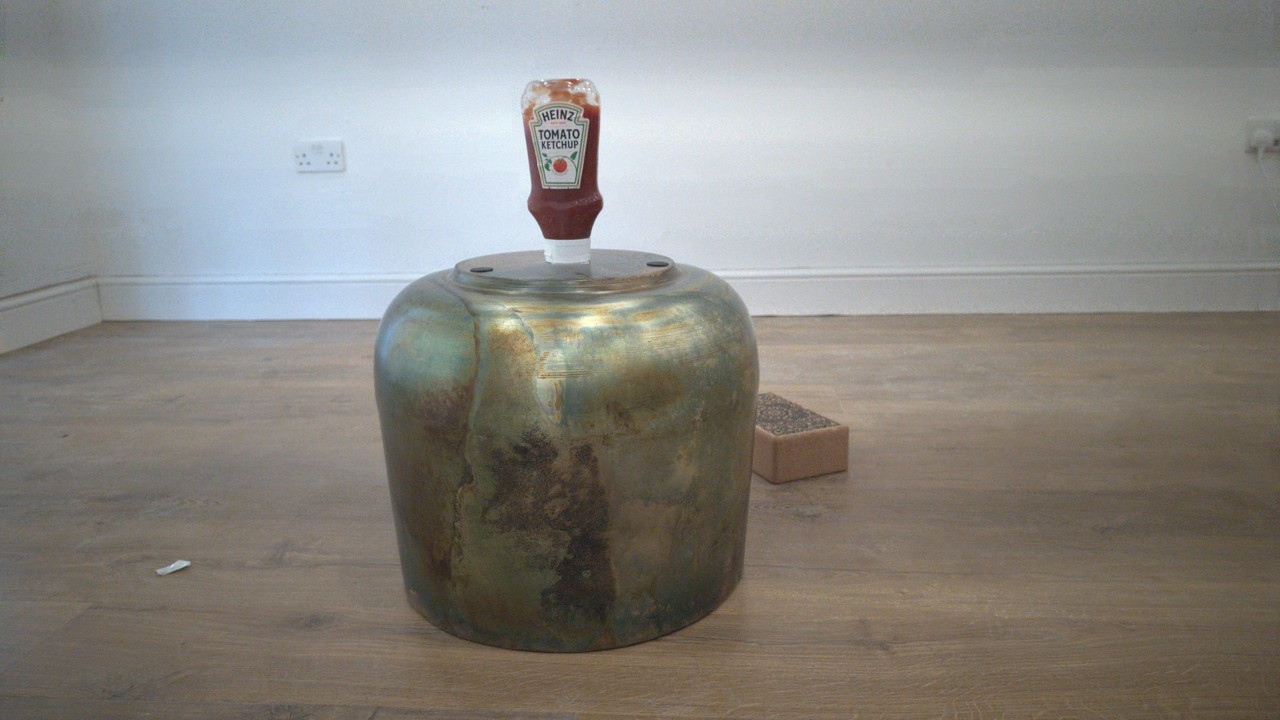
\includegraphics[width=0.42\textwidth]{figures/rawcapdev/wb_after.jpg}\hfill
  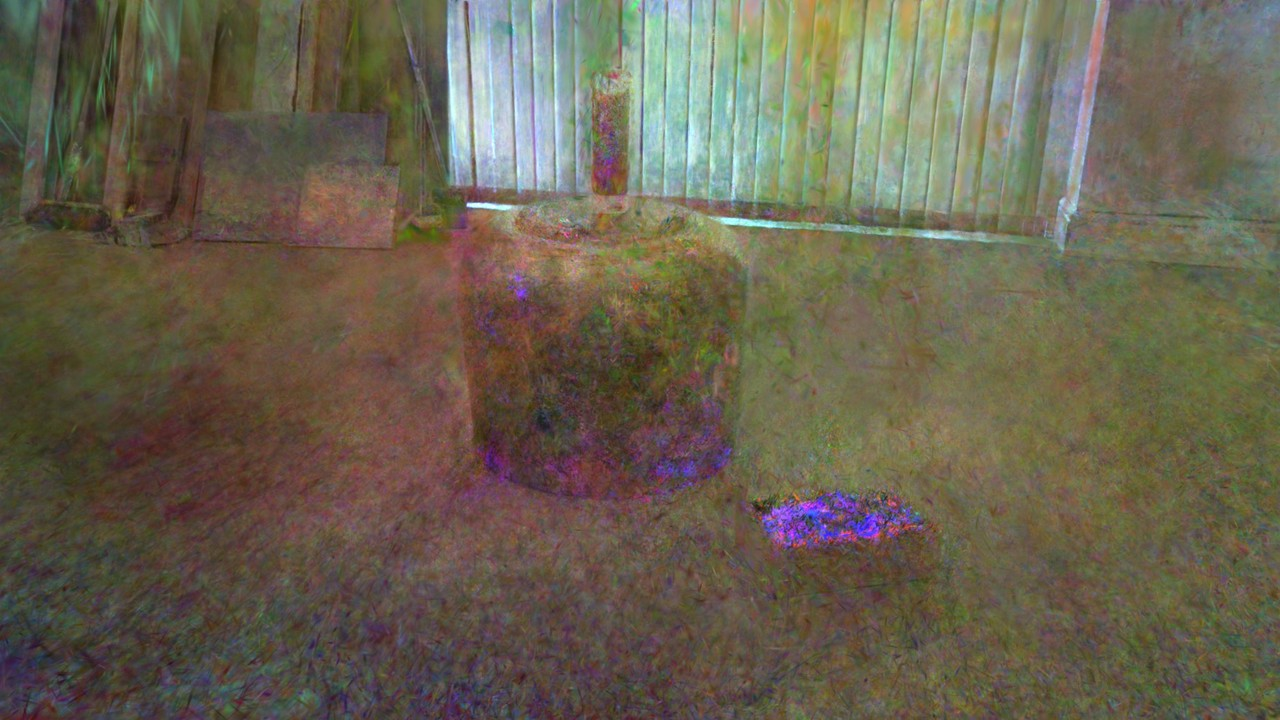
\includegraphics[width=0.52\textwidth]{figures/rawcapdev/splat.jpg}
  \caption{\textbf{Scene track on raw stills.} Left: a decoded frame with camera white
  balance applied (neutral gallery walls). Right: the LichtFeld-native 4M-Gaussian splat
  of the captured room, rendered from a held-out camera pose. Residual floater haze is
  capture-limited, consistent with Result~6.}
  \label{fig:rawcap_scene}
\end{figure}

\subsection{Object: image-to-3D game asset}

Rather than isolate object Gaussians (segmentation quality remained the limiter --- see
below), the hero object was reconstructed from a single clean SAM crop through the
TRELLIS.2 image$\rightarrow$3D path: shape diffusion to a 274k-vertex mesh, then a 4096
PBR texture bake (Figure~\ref{fig:rawcap_object}). Its world position was recovered
from the \emph{convergence of the camera optical axes} (all frames orbit and
point at the subject), and it was staged in a Blender exhibit scene carrying \code{v2g:*}
lineage metadata (source capture, method, vertex count, world centre, interaction) and
exported as a metadata-tagged GLB.

\begin{figure}[htbp]
  \centering
  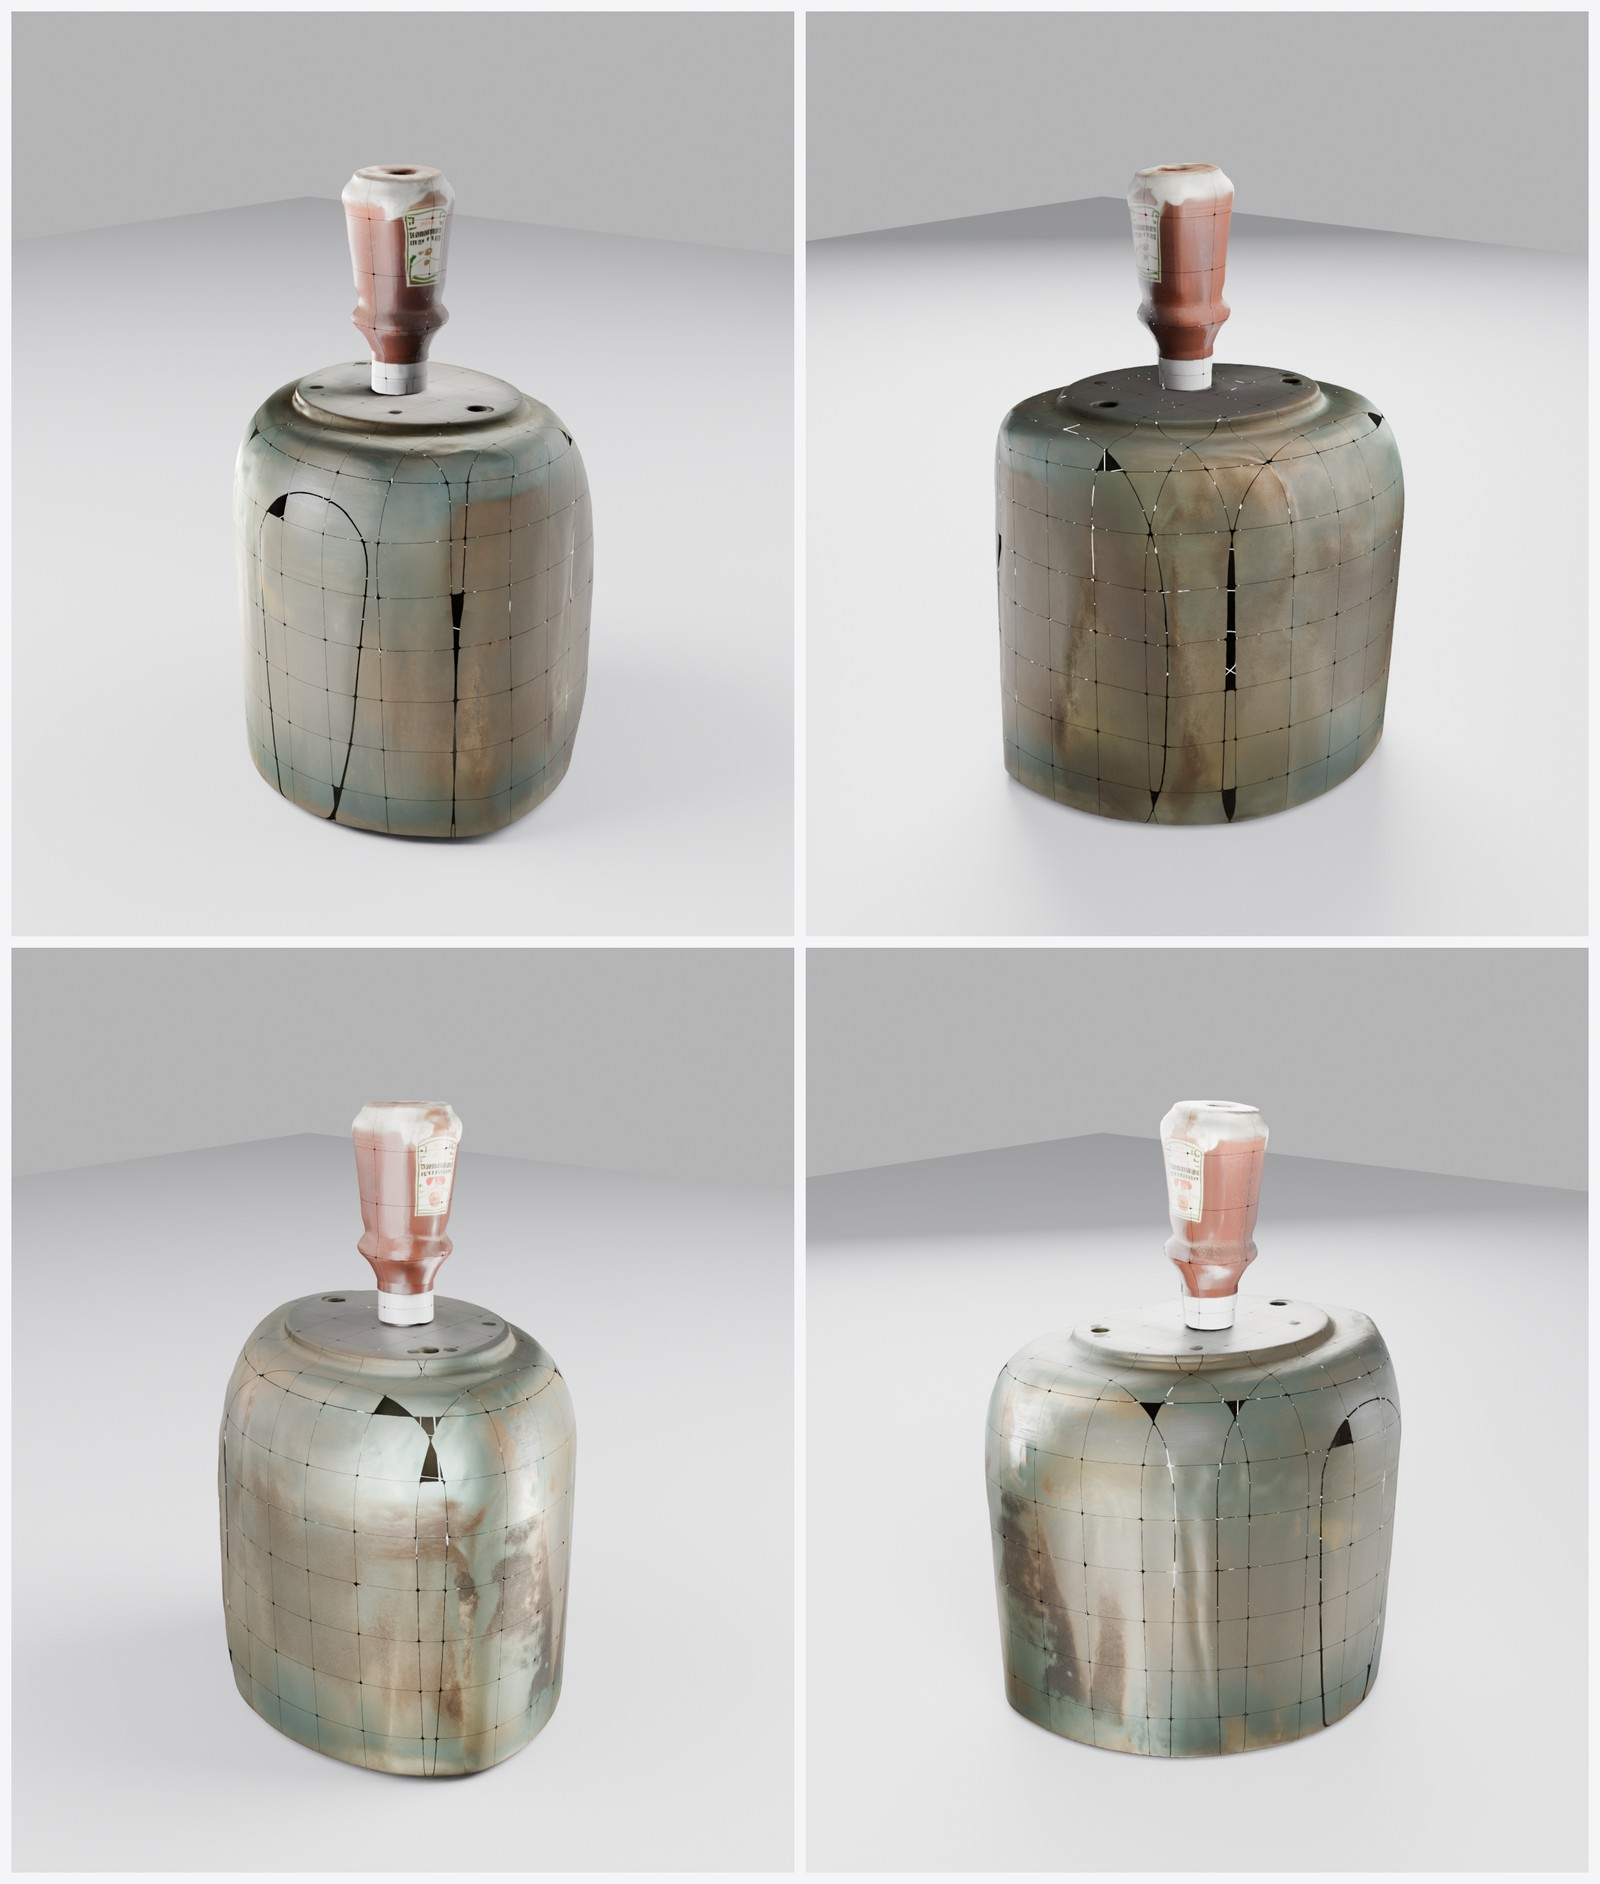
\includegraphics[width=0.56\textwidth]{figures/rawcapdev/object_mesh.jpg}\hfill
  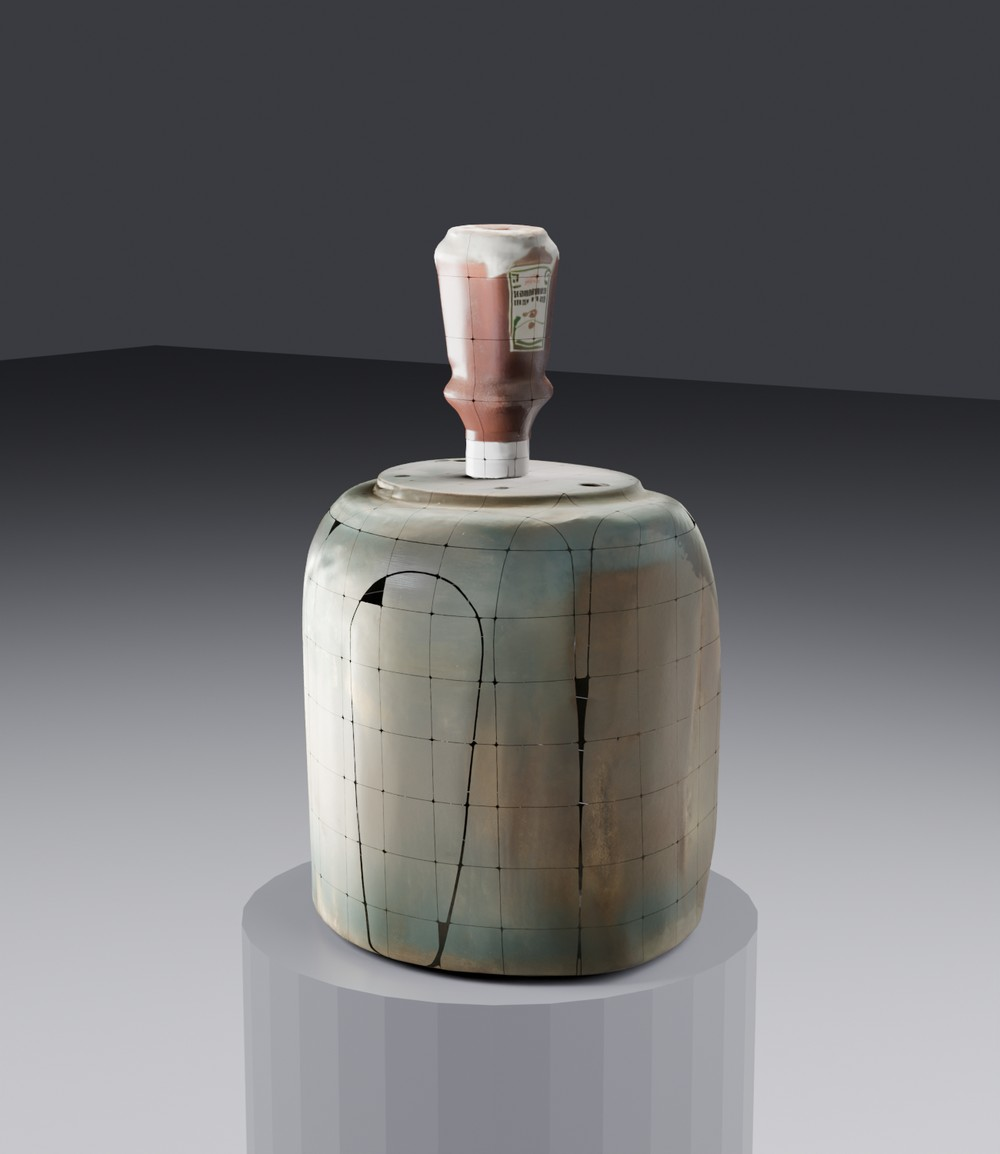
\includegraphics[width=0.40\textwidth]{figures/rawcapdev/exhibit.jpg}
  \caption{\textbf{Object track.} Left: the TRELLIS.2 image$\rightarrow$3D mesh (274k
  verts, 4096 PBR texture), orbit views. Right: the object staged as a game-ready asset
  with \code{v2g:*} metadata. Far-face texture seams are expected single-view artefacts.}
  \label{fig:rawcap_object}
\end{figure}

\subsection{Failures found by running it, and fixed}

Running the pipeline on real data surfaced six defects that unit tests had not; each was
fixed and, where it was a runtime environment fix, codified back into the build:

\begin{itemize}
  \item \textbf{White balance} --- decode applied a fixed daylight balance (orange cast);
        fixed to the camera's as-shot balance.
  \item \textbf{Undistortion size} --- \texttt{image\_undistorter} omitted
        \texttt{max\_image\_size}, producing 36\,MP training images that starved the GPU;
        capped at 2000\,px.
  \item \textbf{Preview renderer SIGFPE} --- \texttt{cameras.bin} width/height are
        \texttt{uint64}, not \texttt{int32}; the wrong read gave \texttt{render\_h=0} and
        a divide-by-zero in the rasteriser.
  \item \textbf{SfM plugin self-clobber} --- the bundled SplatReady plugin overwrote its
        own config mid-run (a status-file naming collision) and exited 0 on failure;
        routed to a transparent direct-COLMAP path instead.
  \item \textbf{Web API dead on arrival} --- an adversarial QE agent found that the four
        new Flask blueprints were imported from the wrong module path and silently
        skipped, so the entire consolidated API returned 404; fixed and verified (37
        routes register).
  \item \textbf{drtk torch-ABI drift} --- TRELLIS.2's PBR texture bake failed because a
        pinned \texttt{drtk} wheel (built for torch~2.11) mismatched the image's
        torch~2.12; the ComfyUI entrypoint now self-heals by rebuilding \texttt{drtk}
        from source against the installed torch.
\end{itemize}

\subsection{Consolidated web control surface}

The run also validated the consolidated web service (ADR-023): a loopback-only Flask
control surface (\code{127.0.0.1:7860}, reached over an SSH tunnel) providing a per-run
file browser with previews, a streamed per-run zip download, a Gaussian-splat viewer, and
an object \code{<model-viewer>} --- all vendored offline (no CDN) for an air-gapped
appliance. The 3DGS-viewer and object-mesh serving paths were exercised against the
\texttt{rawcapdev} outputs.

\subsection{Residual limitation}

SAM3 concept segmentation still returns coarse bounding boxes rather than per-object
silhouettes, so automated per-object Gaussian isolation and precise in-room placement
remain a follow-up; the interim object path (SAM/box crop $\rightarrow$ TRELLIS.2
image$\rightarrow$3D) is what produced the result above. This is a segmentation-quality
limitation, not a reconstruction limit.

% ─────────────────────────────────────────────────────────────────────────────
\section{Summary of Validated Capabilities}
\label{sec:results:summary}

Table~\ref{tab:validated} summarises the validation status of each pipeline component as
of June 2026.  The taxonomy is consistent with the prior \texttt{main\_v4.tex} report:
\textbf{validated} (run on real data, result confirmed), \textbf{in progress} (built,
not exercised end-to-end on the reference run), \textbf{designed} (specified, not built).

\begin{table}[ht]
\centering
\small
\caption{Vitrine component validation status, June 2026 (dreamlab reference run).}
\label{tab:validated}
\begin{tabular}{p{0.44\linewidth} p{0.13\linewidth} p{0.35\linewidth}}
\toprule
\textbf{Component} & \textbf{Status} & \textbf{Evidence / note} \\
\midrule
Frame gate: MUSIQ NR-IQA                   & validated   & MUSIQ $\approx$31 on dreamlab; correctly above abandon threshold. \\
Frame gate: directional $\lambda_2$ metric & validated   & 4 unit tests pass; recapture flag issued. \\
Blur-aware FIFO sampler                    & validated   & $+$20--38\% bottom-quartile sharpness on dreamlab. \\
COLMAP SfM (GPU SIFT)                      & validated   & 600/600 registered, 1.03~px mean reproj. \\
LichtFeld 3DGS training (ImprovedGS+)      & validated   & 2.48M Gaussians; \texttt{splat\_30000.ply}. \\
SuperSplat floater removal                 & validated   & 2.48M $\rightarrow$ 1.55M. \\
NanoGS splat-in-UE (UE 5.8 recompile)     & validated   & Full scene stands in editor (Fig.~\ref{fig:nanogs_room}). \\
TSDF mesh extraction (ScalableTSDFVolume)  & validated   & Stable; 2DGS parity confirmed. \\
2DGS mesh extraction                       & validated   & 69.7\% planarity --- capture-limited, not extractor. \\
Mesh clean + xatlas bake + FBX             & validated   & Working recipe; smooth=0 required. \\
UE room mesh import (Nanite)               & validated   & FBX import with baked albedo. \\
SAM3 concept segmentation                  & validated   & 5 objects; bf16 dtype bug patched. \\
TRELLIS.2 hull\_e2e (objects)              & validated   & Chair, vacuum, toolbox GLBs; UE placed. \\
UE object FBX import + placement           & validated   & Pre-scaled offline; no actor-query API. \\
ArtiFixer sidecar standup (Ada sm\_89)     & validated   & 45.5~GB peak; 3 OOM walls fixed. \\
ALIKED + LightGlue matching                & in progress & Config wired; blocked on libcudnn.so.9. \\
3dgs-deblur / BAD-Gaussians                & in progress & In component menu; not run on dreamlab. \\
ArtiFixer enhance on a real scene          & in progress & Gated on per-scene evidence (ADR-020). \\
SAM3D-Objects                              & designed    & Staged; not yet run. \\
\bottomrule
\end{tabular}
\end{table}

The integrated dreamlab scene --- NanoGS splat room with embedded object FBXs --- is the
headline deliverable of the reference run and is documented in
Figures~\ref{fig:nanogs_room} and~\ref{fig:scene_integrated}.  The mesh-track result
(Table~\ref{tab:planarity}, Figure~\ref{fig:ue_come}) is reported as a
\emph{negative result}: it is the empirical evidence that motivates the splat-hero
architecture and the recapture recommendation, not a failure to be apologised for.  The
two results together --- splat-hero works, mesh is capture-limited --- constitute a
\emph{complete} answer to the question ``what does the dreamlab footage support?''.


% ====================================================================
% Figures — float here, referenced from chapters above
% ====================================================================

% figures.tex — all figures for the Vitrine v5 report
% Include in the main document body with % figures.tex — all figures for the Vitrine v5 report
% Include in the main document body with % figures.tex — all figures for the Vitrine v5 report
% Include in the main document body with \input{figures}
% Assumes \graphicspath{{figures/}} is set in the preamble (relative to report/v5/).
%
% Labels (for \ref / \autoref):
%   fig:router           — capture-adaptive router flowchart
%   fig:component_menu   — component-menu status flowchart
%   fig:architecture     — system architecture (container topology)
%   fig:nanogs_room      — NanoGS real-Gaussian splat render (canonical room hero)
%   fig:scene_integrated — fully integrated UE 5.8 scene (room + objects)
%   fig:objects          — TRELLIS.2 object turnaround sheet (chair)
%   fig:ue_come          — CoMe-TSDF mesh game asset in UE (baseline mesh)
%   fig:ue_nanogs        — NanoGS splat render (dreamlab room, 1920x1080)
%   fig:ue_hero          — Hero perspective render (room + placed objects)
%   fig:ue_dollhouse     — Overhead dollhouse view of integrated UE scene

% ──────────────────────────────────────────────────────────────────────────────
% 1. Capture-adaptive router
% ──────────────────────────────────────────────────────────────────────────────
\begin{figure}[htbp]
  \centering
  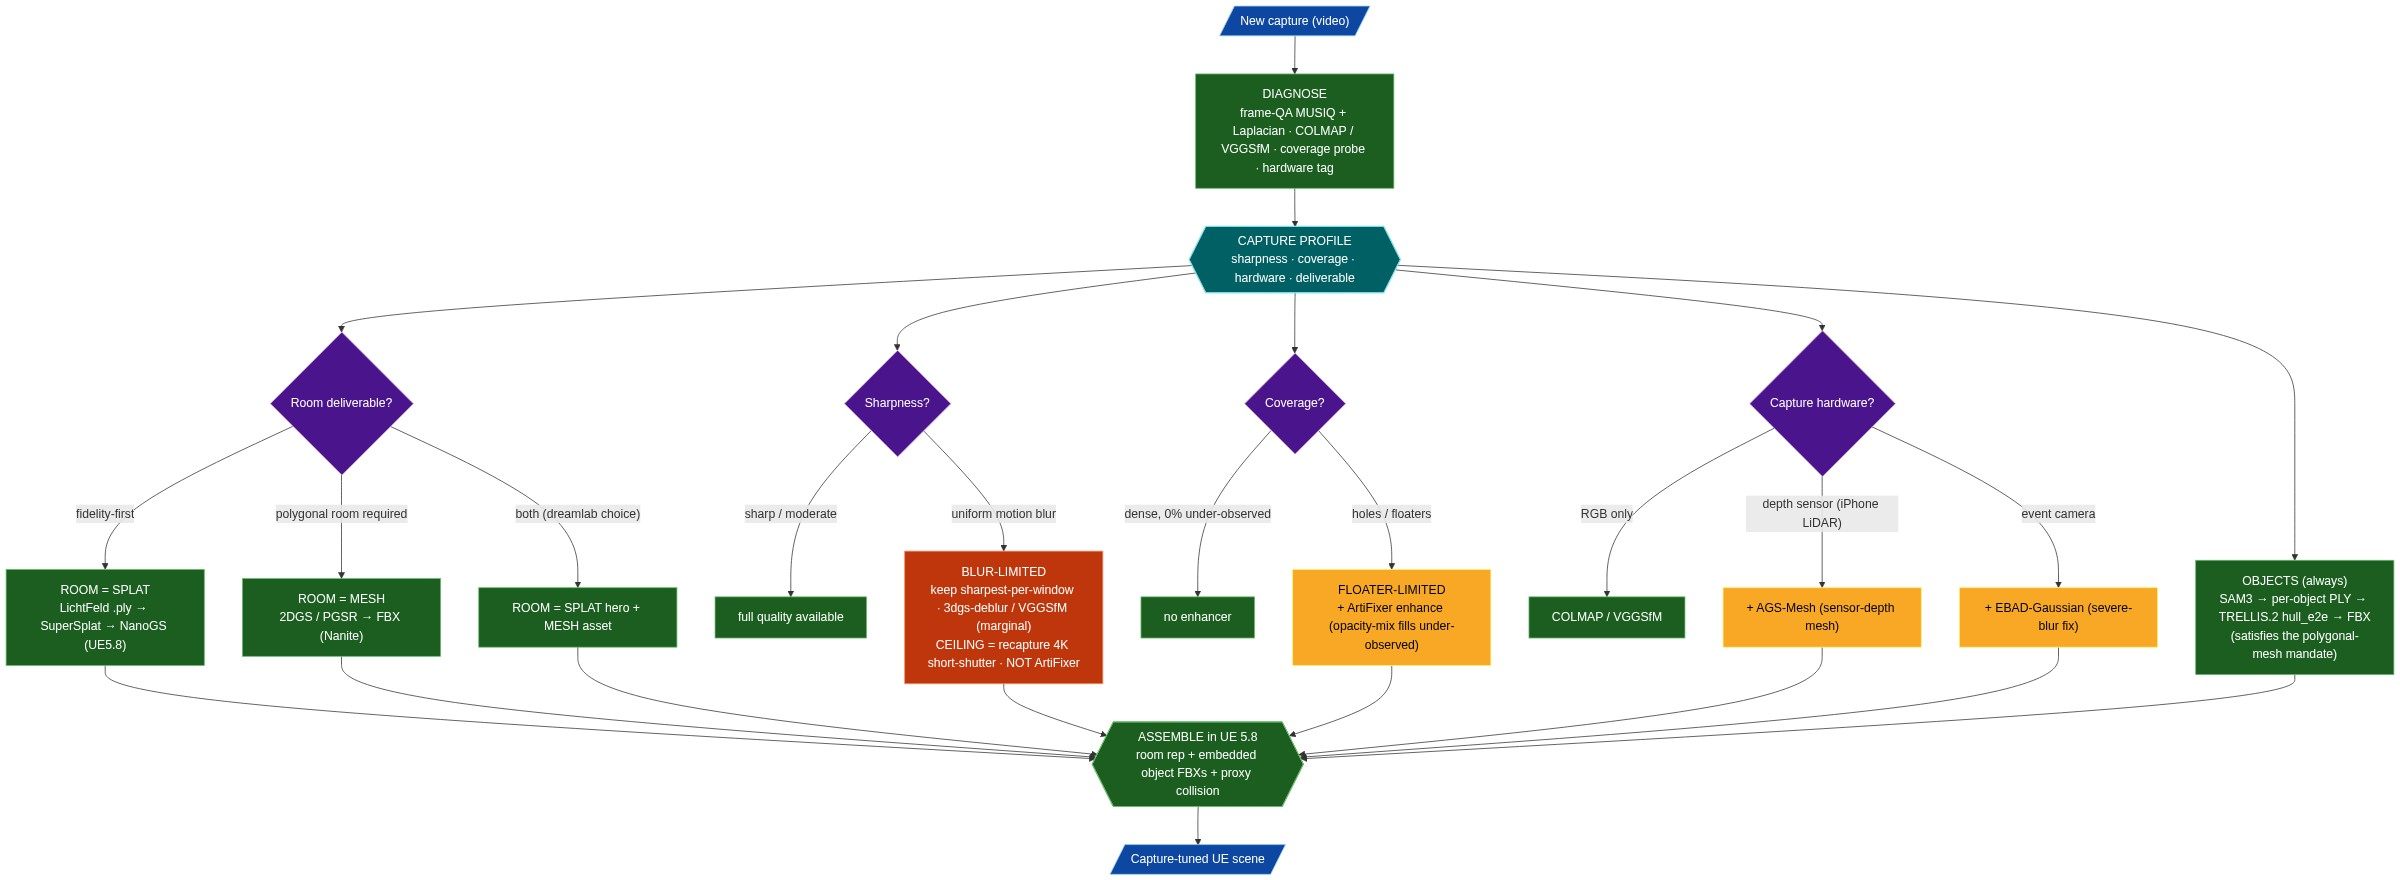
\includegraphics[width=\textwidth]{figures/router.jpg}
  \caption{%
    \textbf{Capture-adaptive router.}
    The pipeline diagnoses each new capture on four axes
    (sharpness via MUSIQ + full-resolution Laplacian, coverage via occupancy probe,
    available hardware, and deliverable type) and selects the configuration that
    fits the bottleneck.
    Green nodes are validated keepers; orange nodes are
    capture-conditional options; red nodes are blur-limited warnings.
    The dreamlab capture routes to Opt\,4 (splat hero + mesh asset + TRELLIS.2 objects)
    with a recapture flag as the quality ceiling.
  }
  \label{fig:router}
\end{figure}

% ──────────────────────────────────────────────────────────────────────────────
% 2. Component-menu flowchart
% ──────────────────────────────────────────────────────────────────────────────
\begin{figure}[htbp]
  \centering
  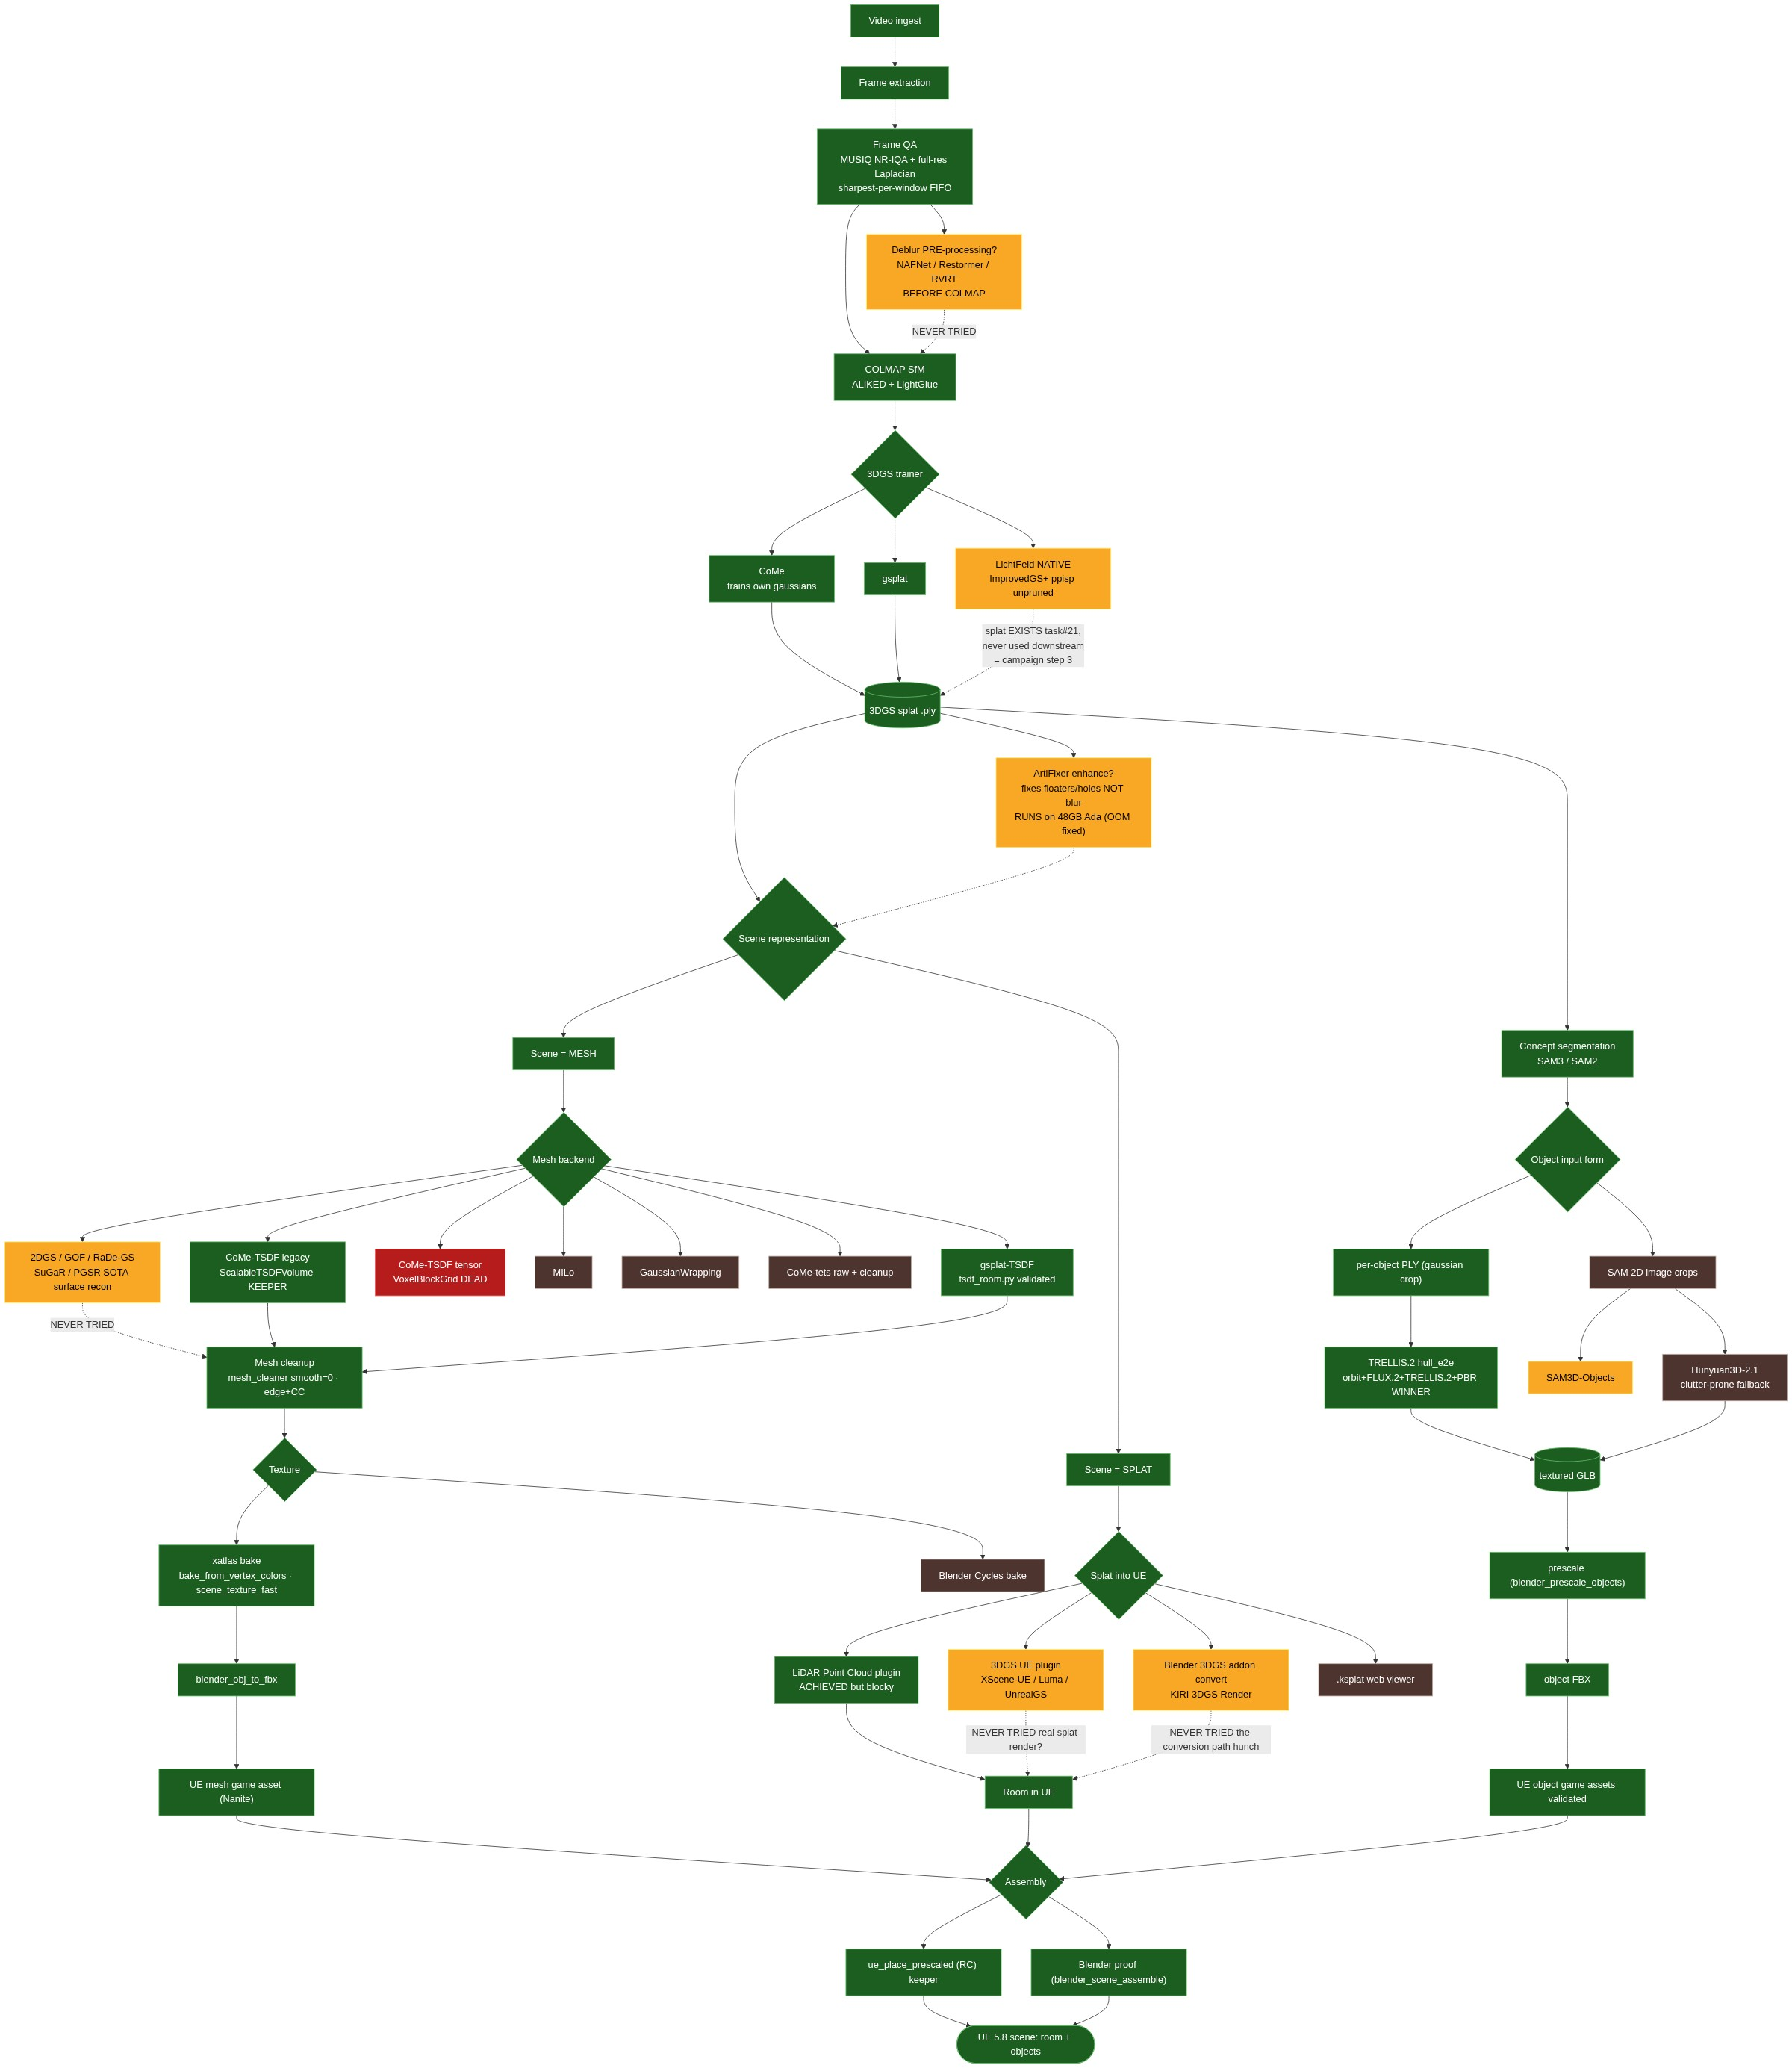
\includegraphics[width=\textwidth]{figures/component_menu.jpg}
  \caption{%
    \textbf{Full component-menu status chart (validated 2026-06-25).}
    Every branch of the Vitrine toolkit from video ingest to UE\,5.8 delivery.
    Colour coding: \emph{green} = validated keeper in active use;
    \emph{brown} = exercised but subordinate / fallback;
    \emph{red} = tried and abandoned;
    \emph{yellow} = plausible, never run.
    The chart is the canonical record of what has and has not been exercised;
    dashed arrows mark paths that remain open research items
    (SAM3D-Objects, BAD-Gaussians deblur, PGSR/2DGS surface reconstruction).
  }
  \label{fig:component_menu}
\end{figure}

% ──────────────────────────────────────────────────────────────────────────────
% 3. System architecture (container topology)
% ──────────────────────────────────────────────────────────────────────────────
\begin{figure}[htbp]
  \centering
  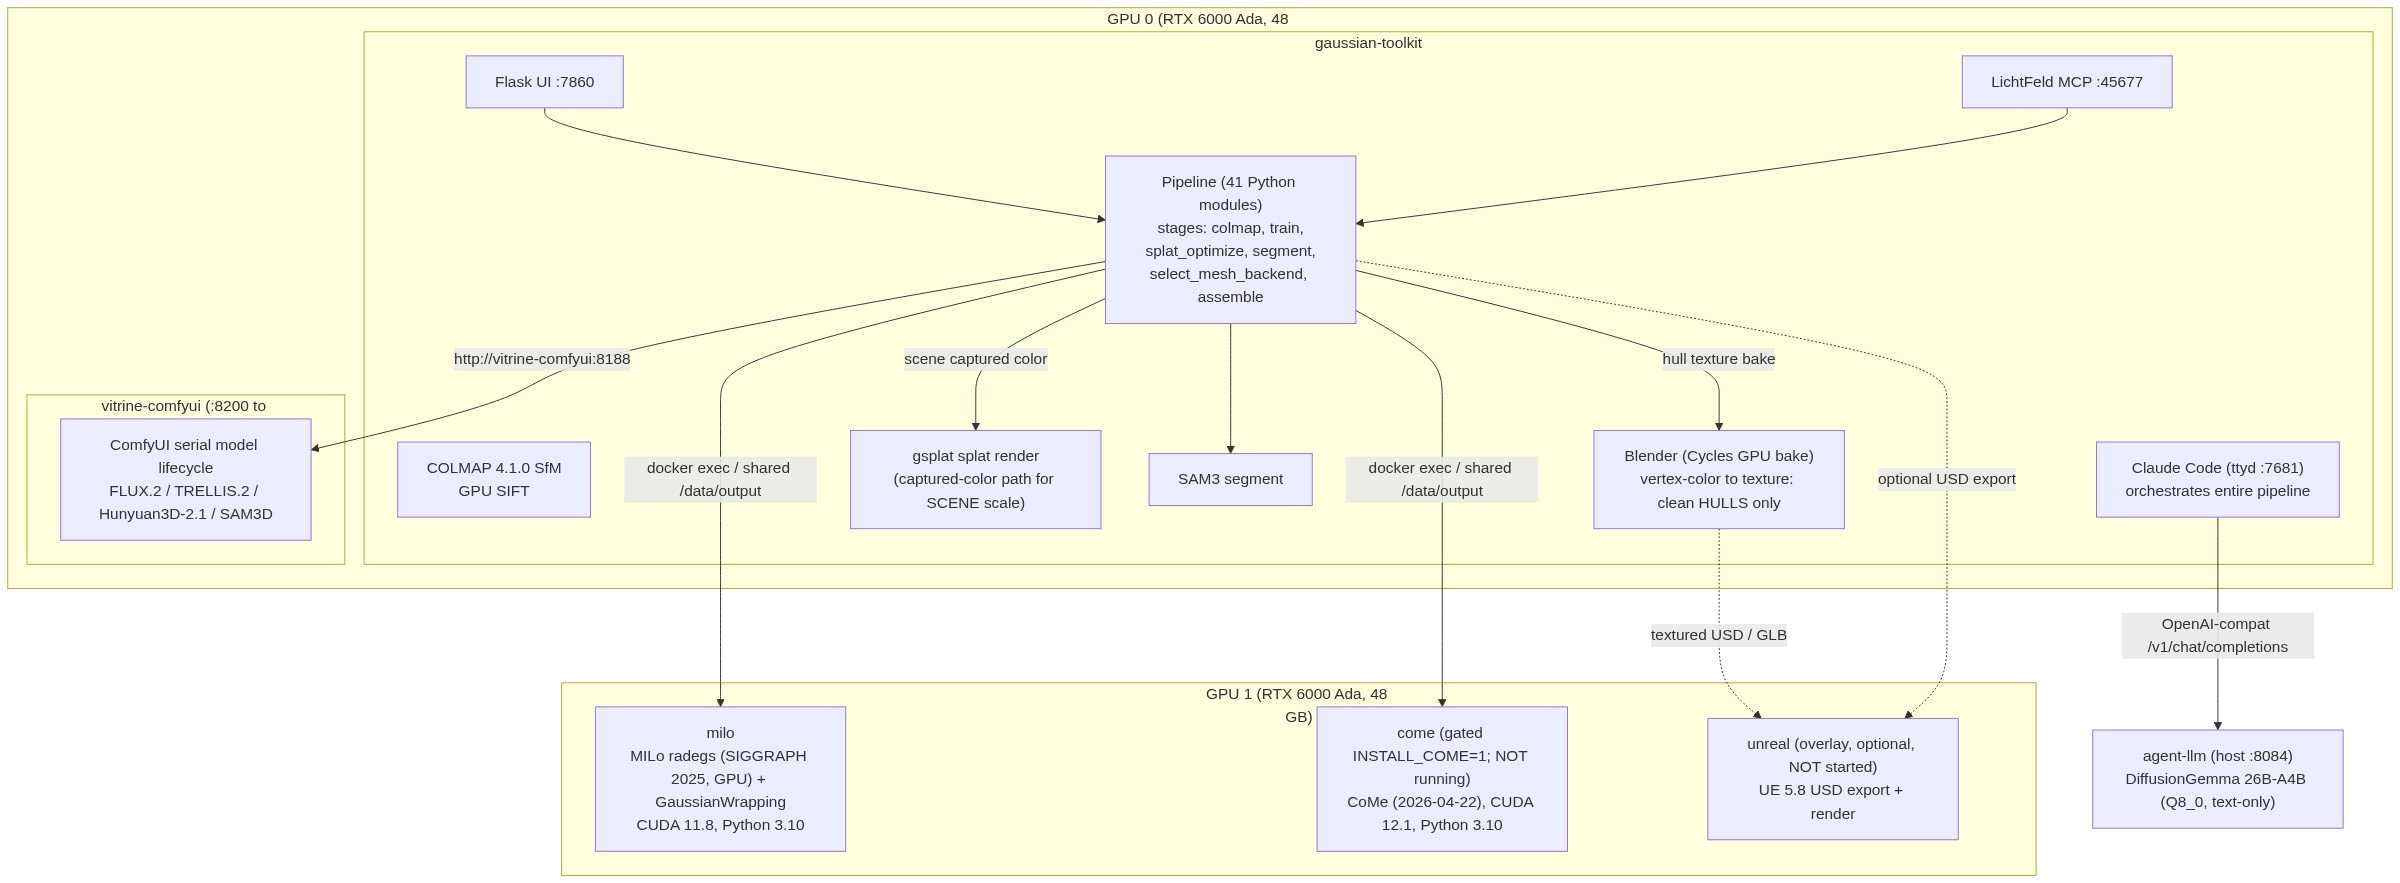
\includegraphics[width=\textwidth]{figures/architecture.jpg}
  \caption{%
    \textbf{Vitrine system architecture — Docker container topology.}
    Two RTX\,6000\,Ada GPUs (48\,GB each) host the six-container stack.
    GPU\,0 runs the \texttt{gaussian-toolkit} orchestrator (COLMAP, LichtFeld
    3DGS, SAM3, Flask\,UI, LichtFeld\,MCP on port\,45677) and
    \texttt{vitrine-comfyui} (FLUX.2\,/\,TRELLIS.2\,/\,Hunyuan3D-2.1, serial
    model lifecycle).
    GPU\,1 hosts the \texttt{milo} sidecar (MILo radegs, CUDA\,11.8) and the
    optional \texttt{come} (CoMe, CUDA\,12.1) and \texttt{unreal} (UE\,5.8)
    overlay containers.
    DiffusionGemma\,26B-A4B runs on the host at port\,8084 as the local text
    reasoner.
    All pipeline containers share \texttt{v2g-net}; the agentbox (Claude Code)
    reaches them via the shared \texttt{visionclaw\_network}.
  }
  \label{fig:architecture}
\end{figure}

% ──────────────────────────────────────────────────────────────────────────────
% 4. NanoGS room splat (docs canonical hero)
% ──────────────────────────────────────────────────────────────────────────────
\begin{figure}[htbp]
  \centering
  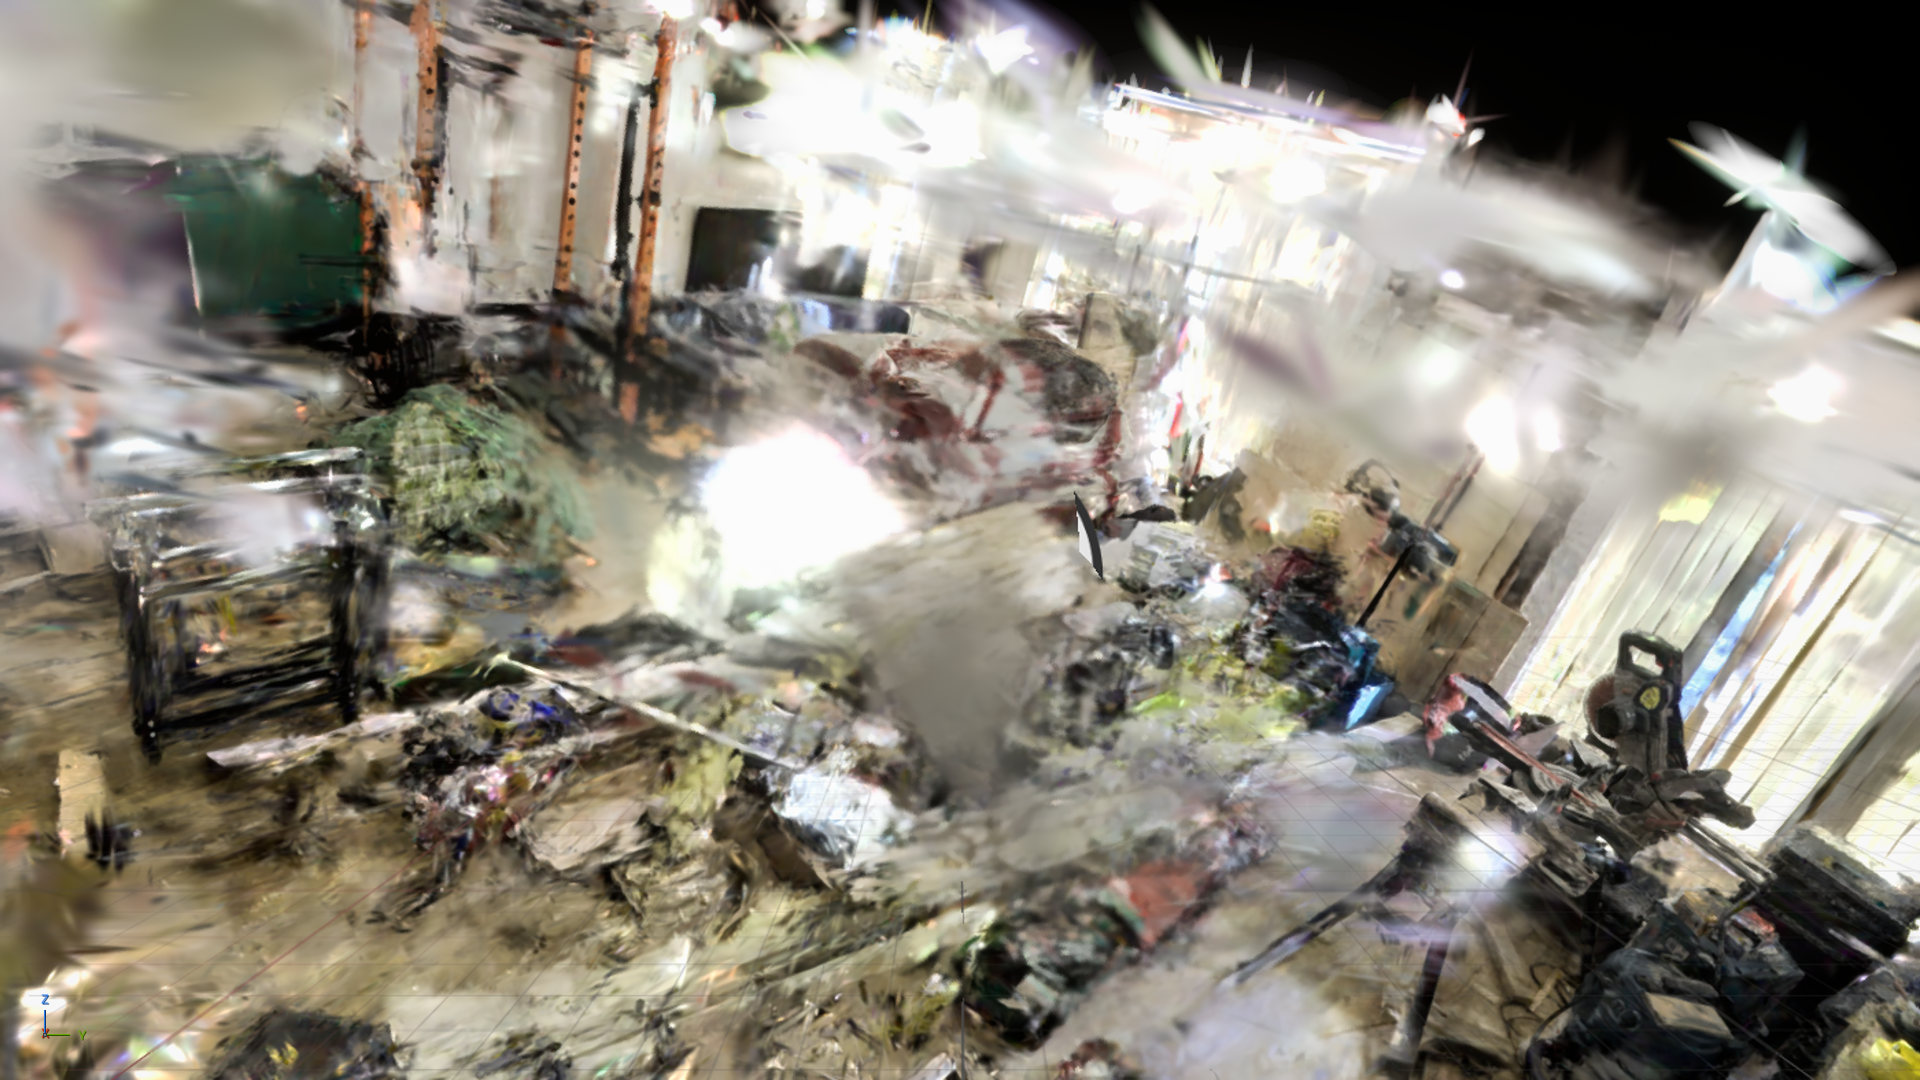
\includegraphics[width=\textwidth]{figures/nanogs_room_splat.png}
  \caption{%
    \textbf{Dreamlab room — NanoGS real-Gaussian splat render (canonical hero).}
    The LichtFeld-native \texttt{splat\_30000.ply}, cleaned via SuperSplat and
    loaded into the NanoGS\,(MIT) UE\,5.8 plugin, rendered at 1920$\times$1080.
    This replaces the earlier LiDAR point-cloud workaround and constitutes
    campaign step\,3: lean-on-LichtFeld native output for the room representation.
    Motion-blur softness in the source splat reflects the dreamlab capture
    constraint (MUSIQ $\approx$ 31); recapture at 4\,K\,/\,short shutter is the
    ceiling lever, not a pipeline limitation.
  }
  \label{fig:nanogs_room}
\end{figure}

% ──────────────────────────────────────────────────────────────────────────────
% 5. Fully integrated UE 5.8 scene
% ──────────────────────────────────────────────────────────────────────────────
\begin{figure}[htbp]
  \centering
  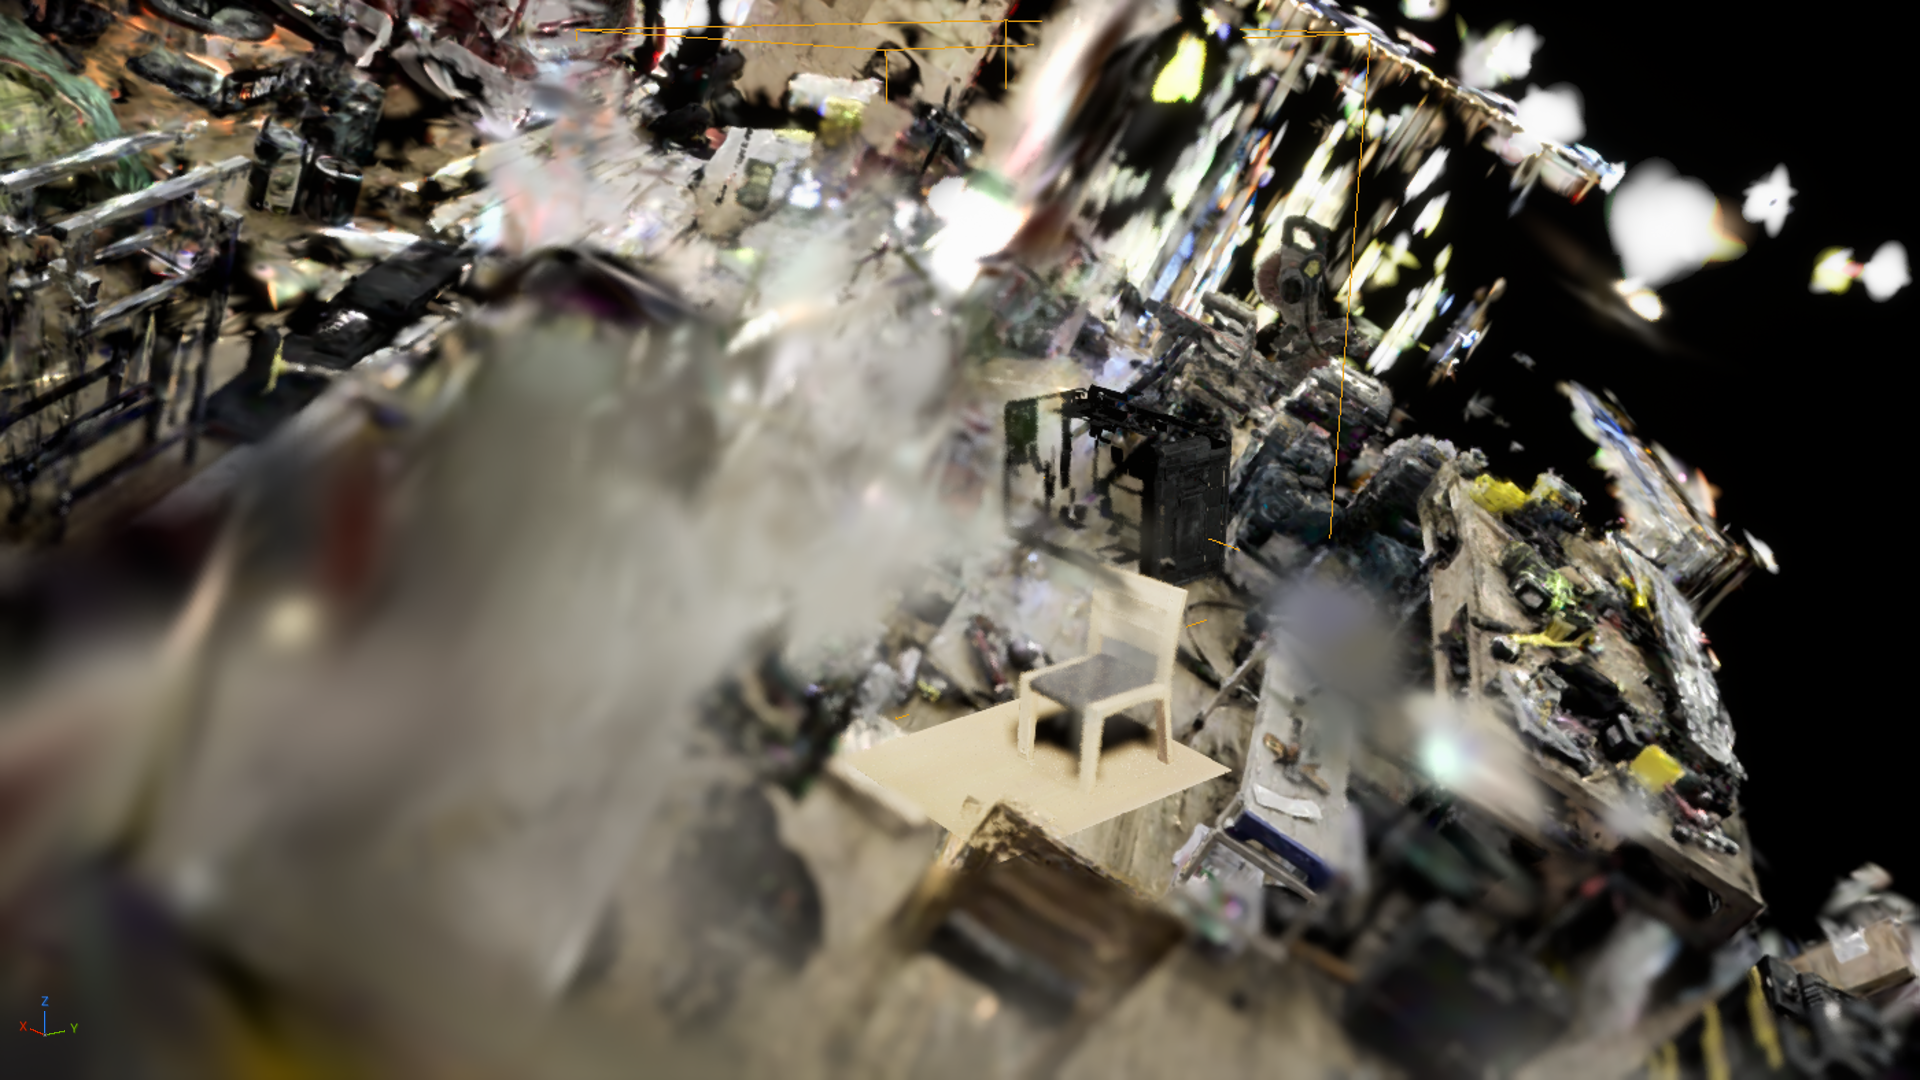
\includegraphics[width=\textwidth]{figures/scene_integrated.png}
  \caption{%
    \textbf{Integrated UE\,5.8 scene — room splat with placed TRELLIS.2 object FBXs.}
    The assembled deliverable: NanoGS splat room (hero representation) with
    chair, vacuum, and toolbox FBXs (TRELLIS.2 \texttt{hull\_e2e},
    prescaled via \texttt{blender\_prescale\_objects}) placed by
    \texttt{ue\_place\_prescaled}.
    Objects are Nanite game assets with baked PBR textures; the room splat
    renders real Gaussians.
    This image is the \emph{docs} canonical integrated-scene reference.
  }
  \label{fig:scene_integrated}
\end{figure}

% ──────────────────────────────────────────────────────────────────────────────
% 6. TRELLIS.2 object turnaround sheet (chair)
% ──────────────────────────────────────────────────────────────────────────────
\begin{figure}[htbp]
  \centering
  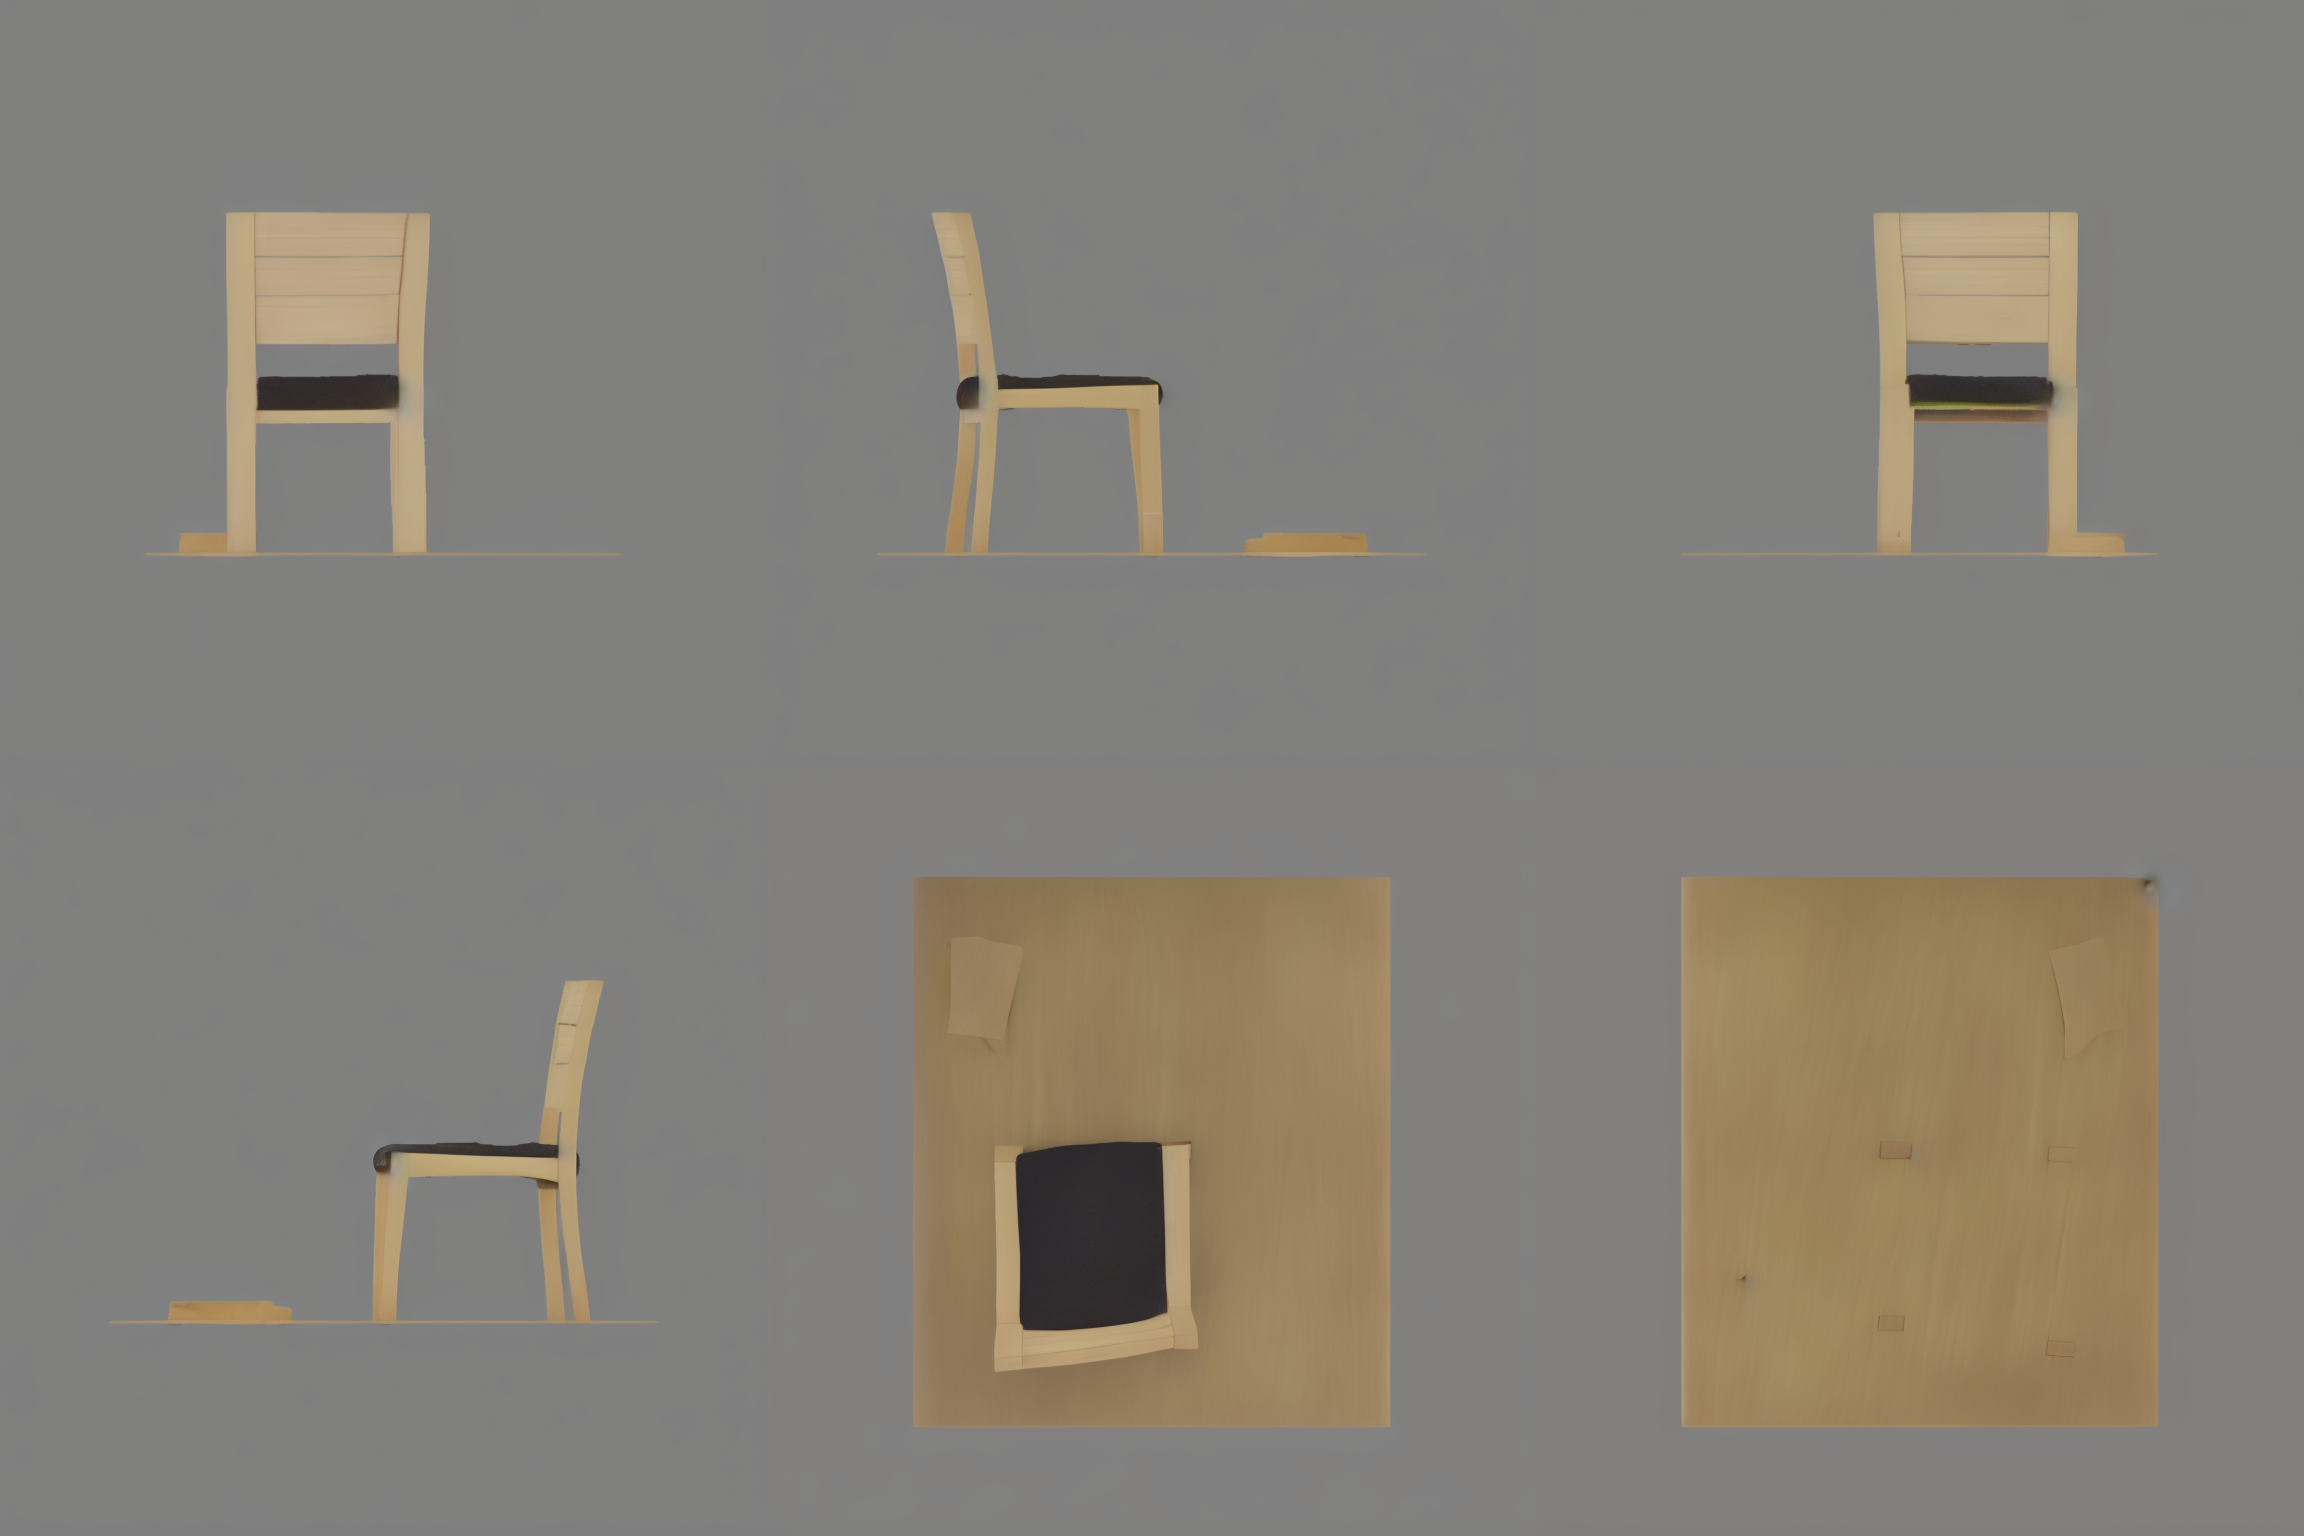
\includegraphics[width=\textwidth]{figures/chair_turnaround_sheet.png}
  \caption{%
    \textbf{TRELLIS.2 object reconstruction — chair turnaround sheet.}
    Multi-view orbit render of the textured GLB mesh produced by the
    \texttt{hull\_e2e} workflow: per-object SAM3 PLY crop $\to$ FLUX.2-dev
    view-inpainting $\to$ TRELLIS.2-4B mesh $\to$ PBR-baked GLB $\to$ FBX
    (Nanite game asset).
    The chair is rated \emph{good}; vacuum and toolbox likewise passed
    the object reconstruction gate (4/8 objects in this batch).
    Resolution: 2304$\times$1536.
  }
  \label{fig:objects}
\end{figure}

% ──────────────────────────────────────────────────────────────────────────────
% 7. CoMe-TSDF mesh in UE (baseline mesh deliverable)
% ──────────────────────────────────────────────────────────────────────────────
\begin{figure}[htbp]
  \centering
  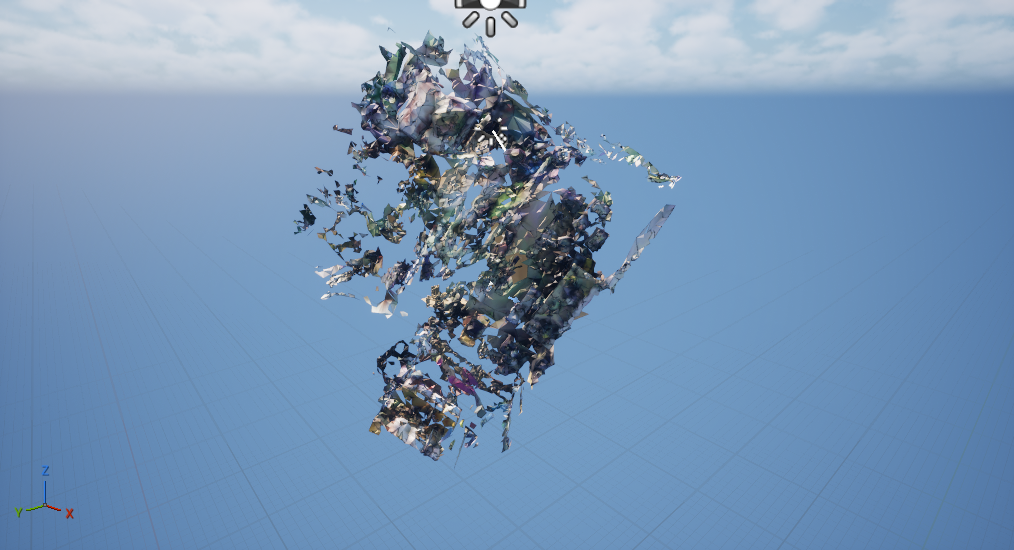
\includegraphics[width=\textwidth]{figures/ue_come_final.png}
  \caption{%
    \textbf{CoMe-TSDF room mesh game asset in UE\,5.8 (baseline mesh deliverable).}
    The scene-mesh branch: CoMe legacy \texttt{ScalableTSDFVolume} extraction,
    \texttt{mesh\_cleaner} (smooth=0, edge-length + connected-component cleanup),
    xatlas bake (\texttt{bake\_from\_vertex\_colors}), \texttt{blender\_obj\_to\_fbx},
    imported as a Nanite mesh.
    Characteristic TSDF blockiness on flat walls is visible; this image
    motivates the re-spine to NanoGS as the default room representation for
    blur-limited captures.
    Resolution: 1014$\times$550.
  }
  \label{fig:ue_come}
\end{figure}

% ──────────────────────────────────────────────────────────────────────────────
% 8. NanoGS splat render (1920×1080 B-view)
% ──────────────────────────────────────────────────────────────────────────────
\begin{figure}[htbp]
  \centering
  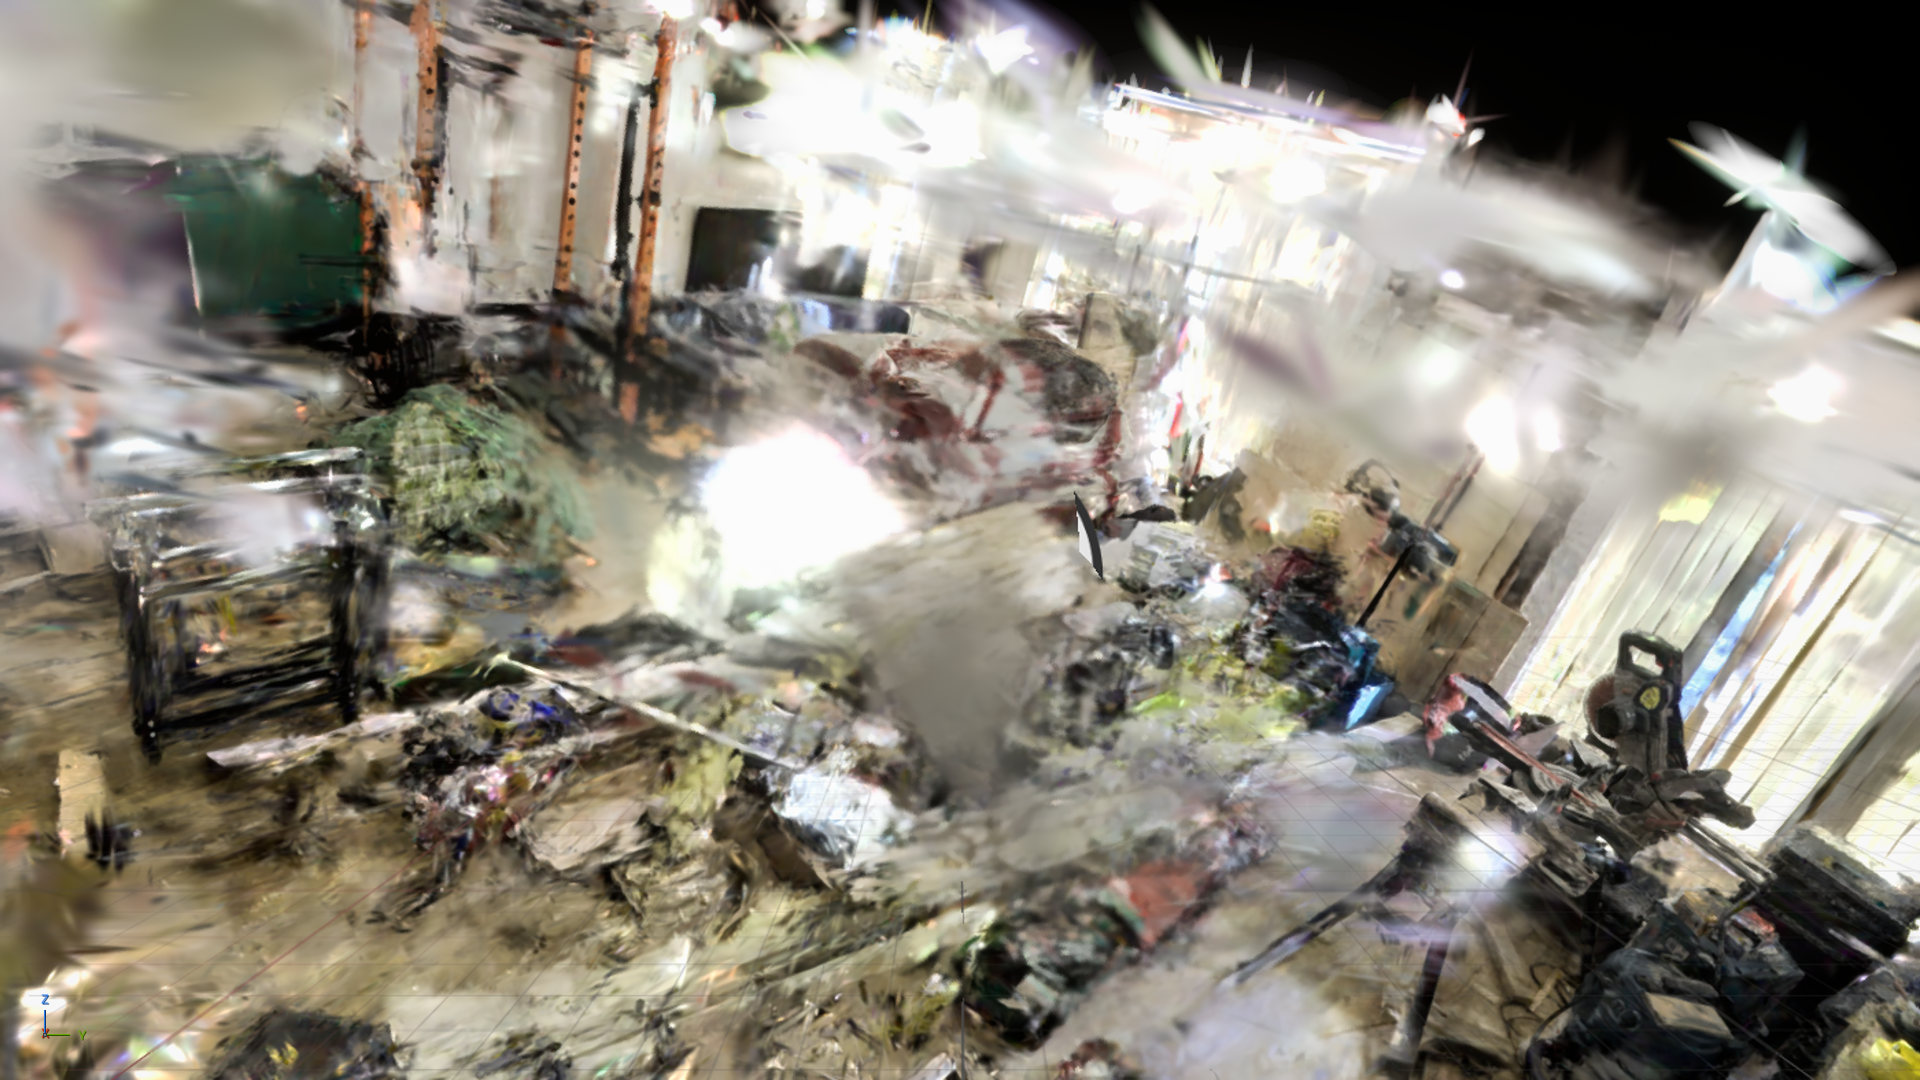
\includegraphics[width=\textwidth]{figures/ue_nanogs_room_B.png}
  \caption{%
    \textbf{NanoGS real-Gaussian splat in UE\,5.8 — interior view (B).}
    Second viewpoint of the NanoGS splat room, demonstrating depth and
    parallax of real Gaussian rendering at 1920$\times$1080.
    Comparison with Figure~\ref{fig:ue_come} illustrates the quality
    improvement of splat-hero over TSDF mesh for a motion-blur-limited
    capture: the splat faithfully preserves captured radiance;
    the mesh introduces geometric artefacts irrelevant to the capture.
  }
  \label{fig:ue_nanogs}
\end{figure}

% ──────────────────────────────────────────────────────────────────────────────
% 9. Hero perspective render (room + placed objects)
% ──────────────────────────────────────────────────────────────────────────────
\begin{figure}[htbp]
  \centering
  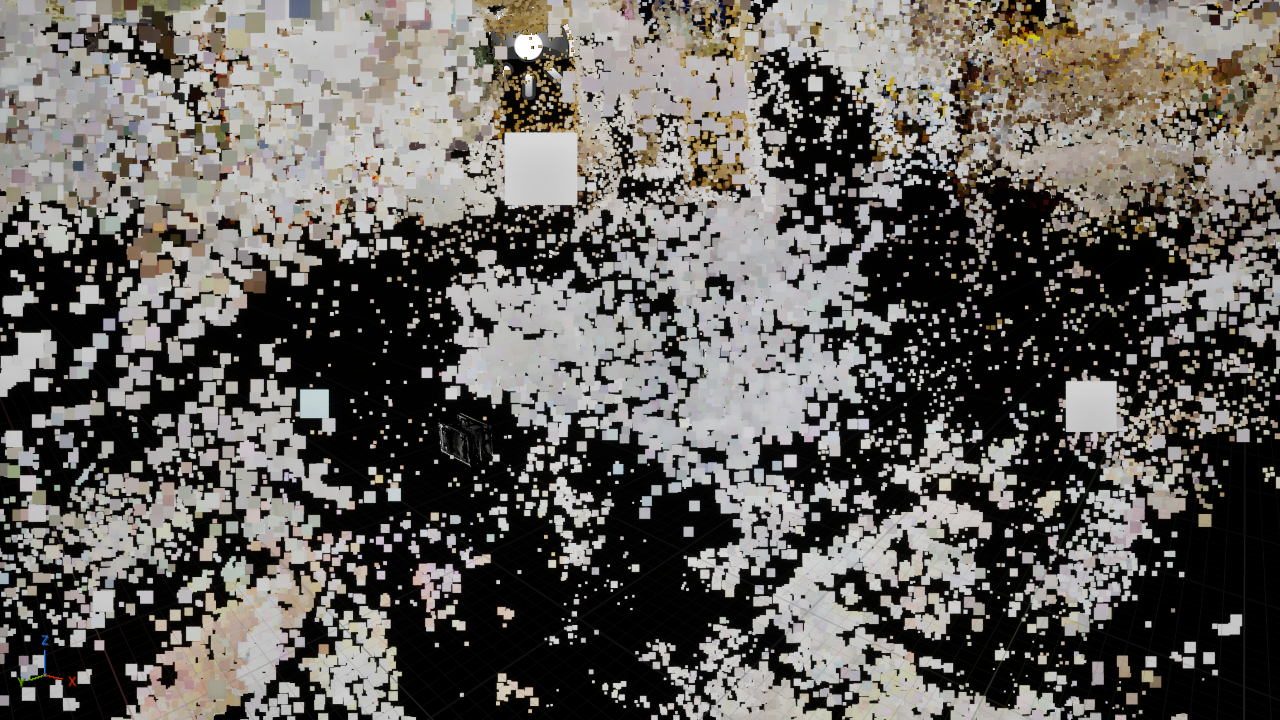
\includegraphics[width=\textwidth]{figures/ue_final_hero.png}
  \caption{%
    \textbf{Hero perspective render — dreamlab room with placed object FBXs.}
    A cinematic view of the assembled UE\,5.8 scene from the validated
    end-to-end run (2026-06-22): TSDF-mesh room (CoMe, pre-NanoGS re-spine)
    with TRELLIS.2 object FBXs placed by \texttt{ue\_place\_prescaled}.
    Resolution: 1280$\times$720.
    Serves as the primary before/after reference for evaluating the
    NanoGS re-spine (Figure~\ref{fig:nanogs_room}).
  }
  \label{fig:ue_hero}
\end{figure}

% ──────────────────────────────────────────────────────────────────────────────
% 10. Overhead dollhouse view
% ──────────────────────────────────────────────────────────────────────────────
\begin{figure}[htbp]
  \centering
  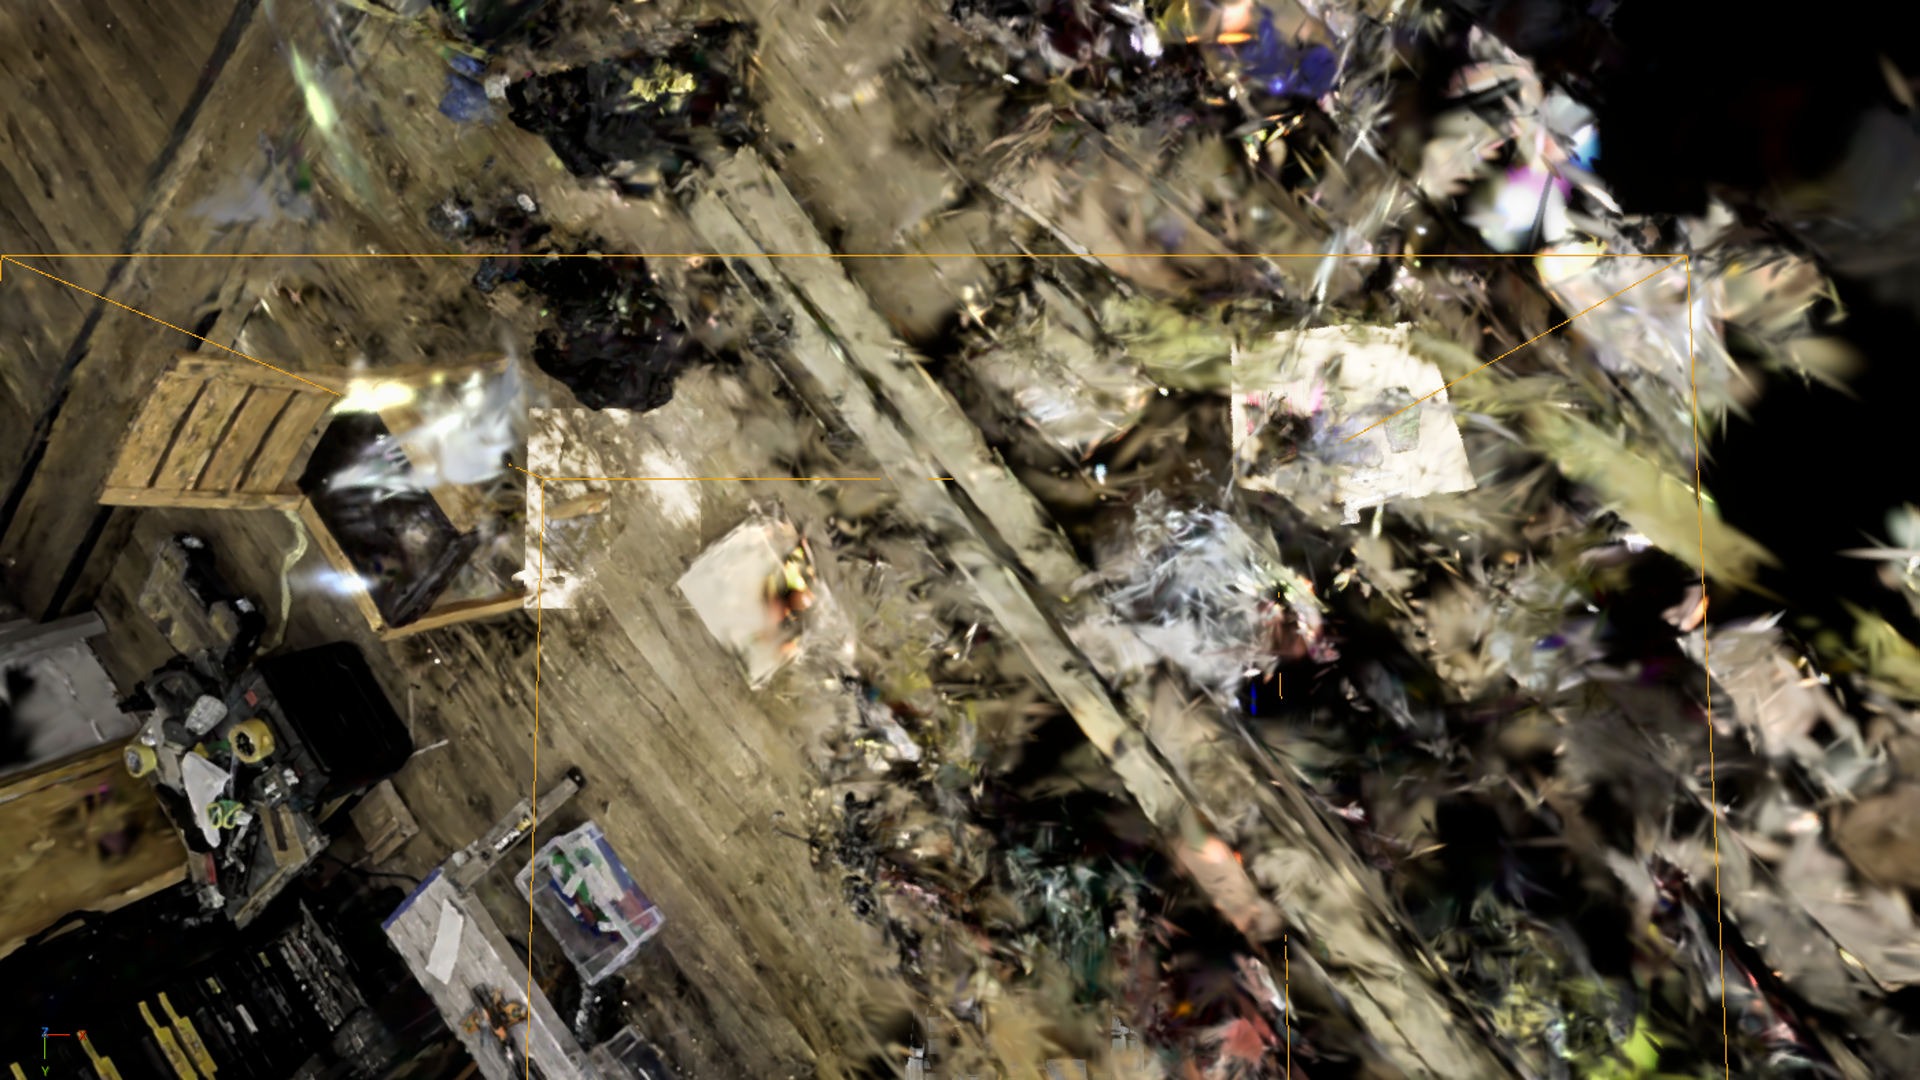
\includegraphics[width=\textwidth]{figures/ue_integrated_dollhouse.png}
  \caption{%
    \textbf{Overhead dollhouse view — integrated UE\,5.8 scene layout.}
    Top-down perspective revealing object placement, room geometry, and
    spatial relationships of the dreamlab scene.
    The dollhouse view is the standard QA checkpoint for scale fidelity
    and object-in-room alignment after \texttt{ue\_place\_prescaled}
    prescaling.
    Resolution: 1920$\times$1080.
  }
  \label{fig:ue_dollhouse}
\end{figure}

% Assumes \graphicspath{{figures/}} is set in the preamble (relative to report/v5/).
%
% Labels (for \ref / \autoref):
%   fig:router           — capture-adaptive router flowchart
%   fig:component_menu   — component-menu status flowchart
%   fig:architecture     — system architecture (container topology)
%   fig:nanogs_room      — NanoGS real-Gaussian splat render (canonical room hero)
%   fig:scene_integrated — fully integrated UE 5.8 scene (room + objects)
%   fig:objects          — TRELLIS.2 object turnaround sheet (chair)
%   fig:ue_come          — CoMe-TSDF mesh game asset in UE (baseline mesh)
%   fig:ue_nanogs        — NanoGS splat render (dreamlab room, 1920x1080)
%   fig:ue_hero          — Hero perspective render (room + placed objects)
%   fig:ue_dollhouse     — Overhead dollhouse view of integrated UE scene

% ──────────────────────────────────────────────────────────────────────────────
% 1. Capture-adaptive router
% ──────────────────────────────────────────────────────────────────────────────
\begin{figure}[htbp]
  \centering
  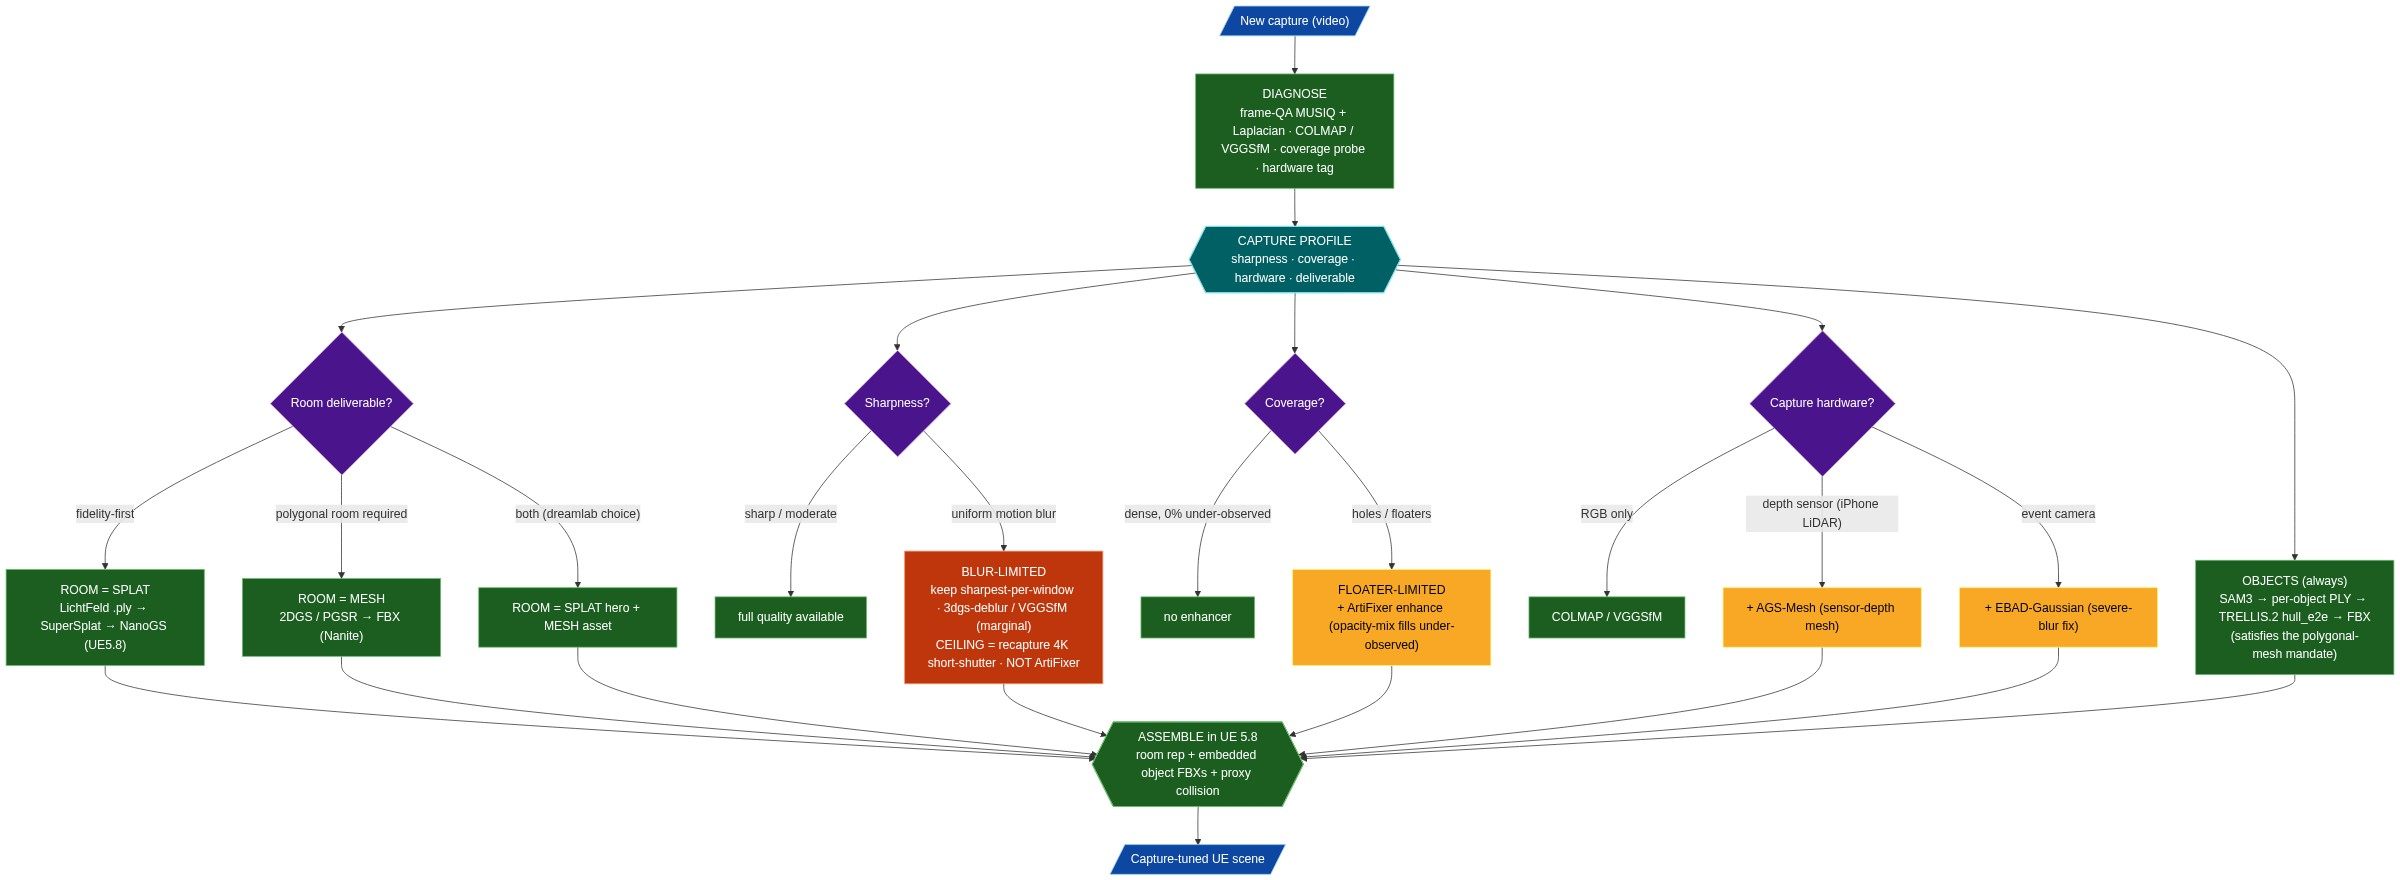
\includegraphics[width=\textwidth]{figures/router.jpg}
  \caption{%
    \textbf{Capture-adaptive router.}
    The pipeline diagnoses each new capture on four axes
    (sharpness via MUSIQ + full-resolution Laplacian, coverage via occupancy probe,
    available hardware, and deliverable type) and selects the configuration that
    fits the bottleneck.
    Green nodes are validated keepers; orange nodes are
    capture-conditional options; red nodes are blur-limited warnings.
    The dreamlab capture routes to Opt\,4 (splat hero + mesh asset + TRELLIS.2 objects)
    with a recapture flag as the quality ceiling.
  }
  \label{fig:router}
\end{figure}

% ──────────────────────────────────────────────────────────────────────────────
% 2. Component-menu flowchart
% ──────────────────────────────────────────────────────────────────────────────
\begin{figure}[htbp]
  \centering
  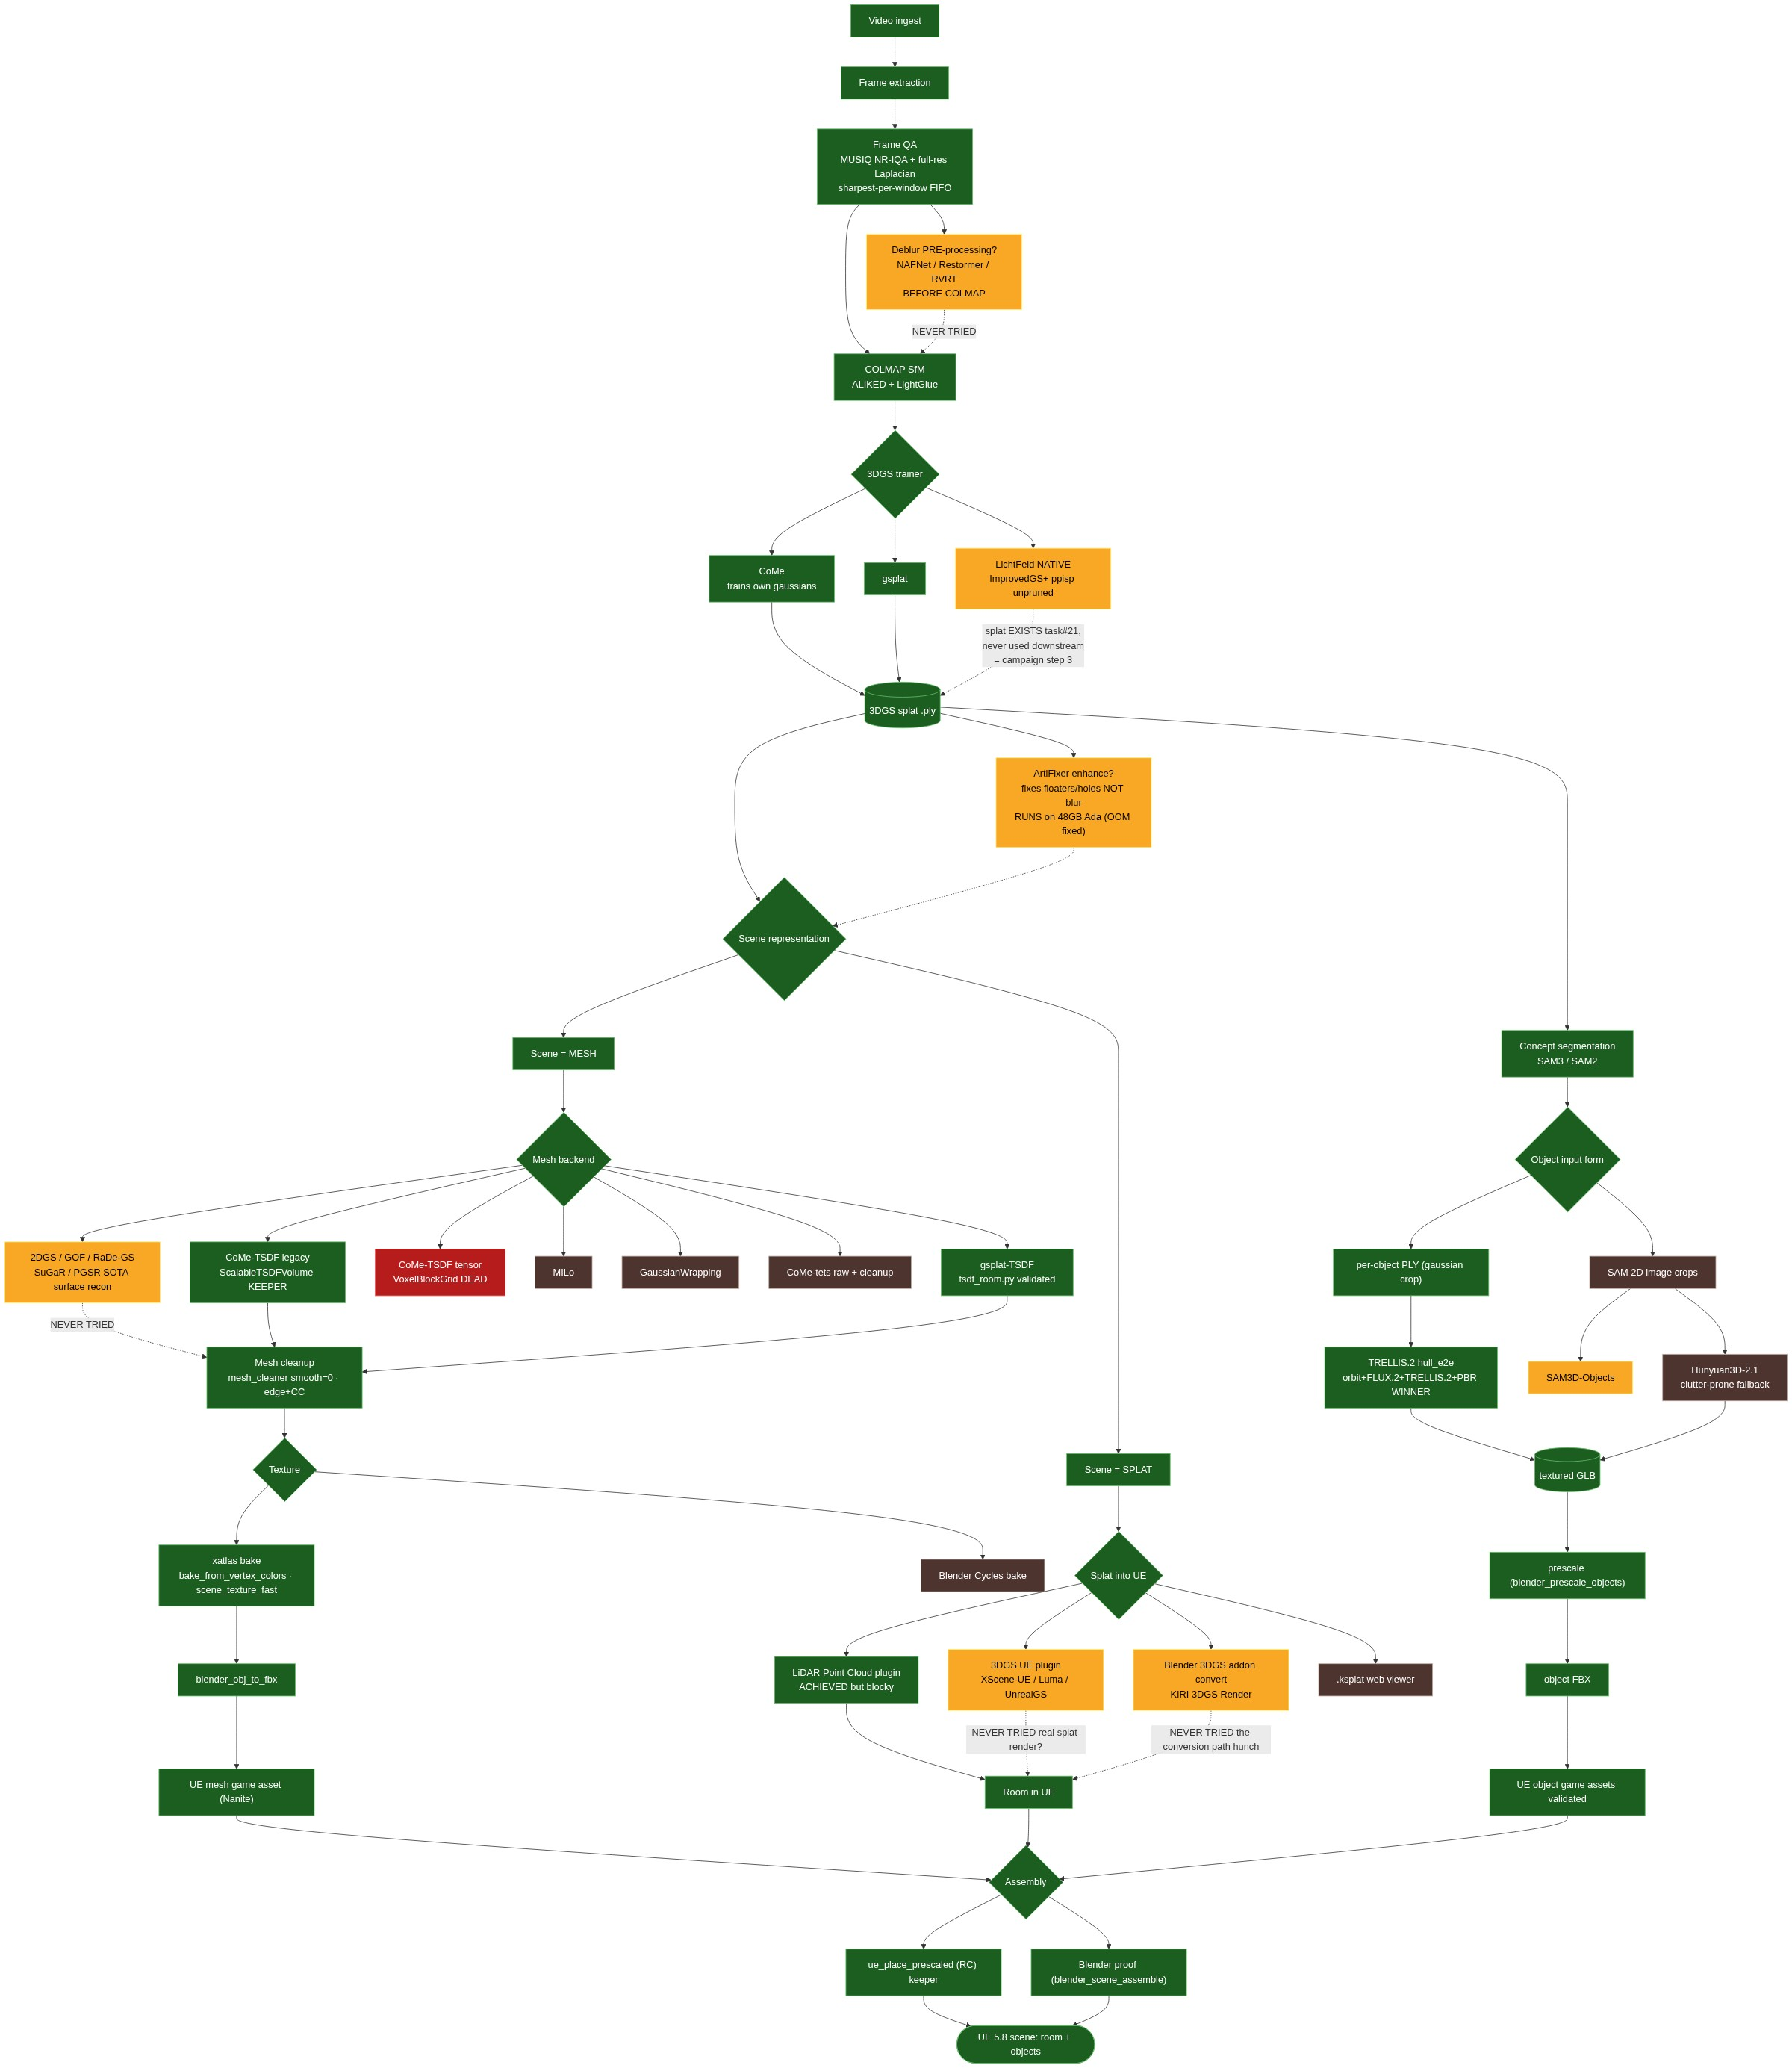
\includegraphics[width=\textwidth]{figures/component_menu.jpg}
  \caption{%
    \textbf{Full component-menu status chart (validated 2026-06-25).}
    Every branch of the Vitrine toolkit from video ingest to UE\,5.8 delivery.
    Colour coding: \emph{green} = validated keeper in active use;
    \emph{brown} = exercised but subordinate / fallback;
    \emph{red} = tried and abandoned;
    \emph{yellow} = plausible, never run.
    The chart is the canonical record of what has and has not been exercised;
    dashed arrows mark paths that remain open research items
    (SAM3D-Objects, BAD-Gaussians deblur, PGSR/2DGS surface reconstruction).
  }
  \label{fig:component_menu}
\end{figure}

% ──────────────────────────────────────────────────────────────────────────────
% 3. System architecture (container topology)
% ──────────────────────────────────────────────────────────────────────────────
\begin{figure}[htbp]
  \centering
  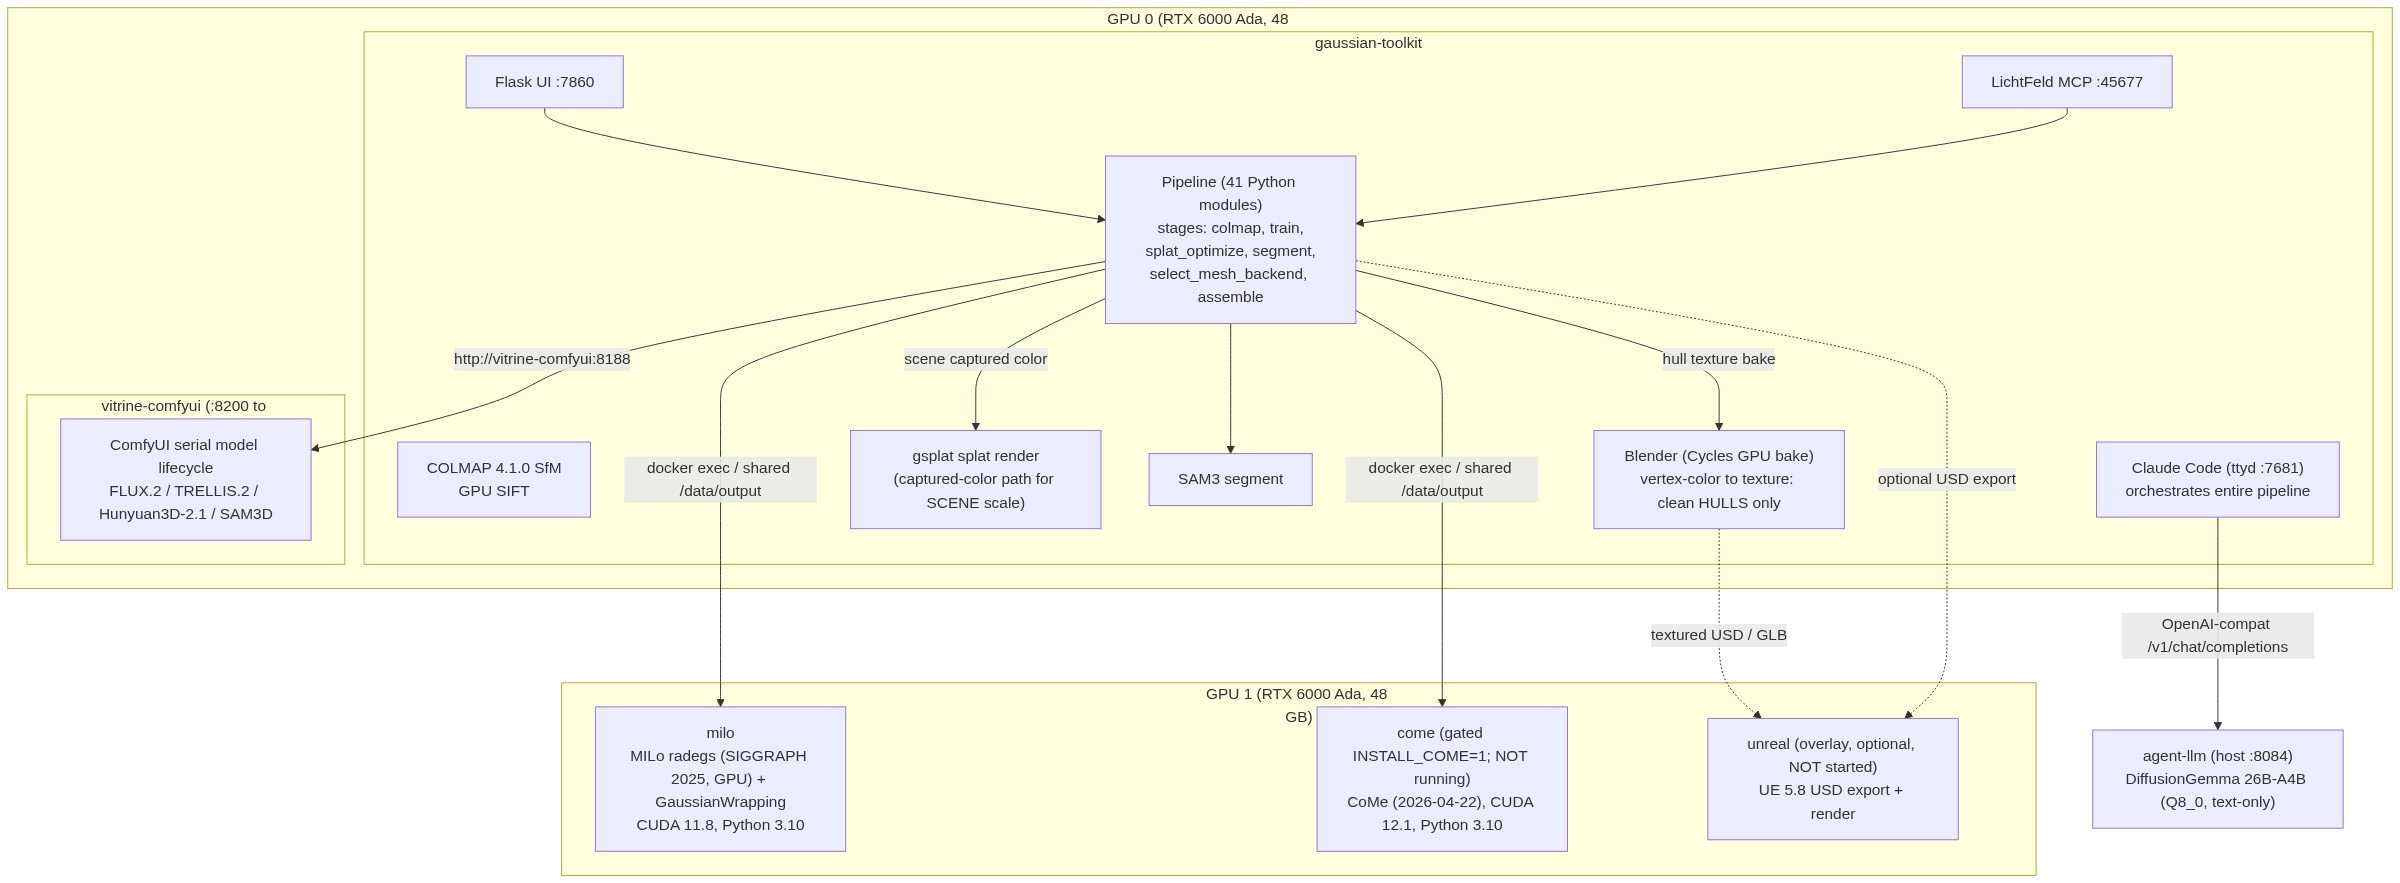
\includegraphics[width=\textwidth]{figures/architecture.jpg}
  \caption{%
    \textbf{Vitrine system architecture — Docker container topology.}
    Two RTX\,6000\,Ada GPUs (48\,GB each) host the six-container stack.
    GPU\,0 runs the \texttt{gaussian-toolkit} orchestrator (COLMAP, LichtFeld
    3DGS, SAM3, Flask\,UI, LichtFeld\,MCP on port\,45677) and
    \texttt{vitrine-comfyui} (FLUX.2\,/\,TRELLIS.2\,/\,Hunyuan3D-2.1, serial
    model lifecycle).
    GPU\,1 hosts the \texttt{milo} sidecar (MILo radegs, CUDA\,11.8) and the
    optional \texttt{come} (CoMe, CUDA\,12.1) and \texttt{unreal} (UE\,5.8)
    overlay containers.
    DiffusionGemma\,26B-A4B runs on the host at port\,8084 as the local text
    reasoner.
    All pipeline containers share \texttt{v2g-net}; the agentbox (Claude Code)
    reaches them via the shared \texttt{visionclaw\_network}.
  }
  \label{fig:architecture}
\end{figure}

% ──────────────────────────────────────────────────────────────────────────────
% 4. NanoGS room splat (docs canonical hero)
% ──────────────────────────────────────────────────────────────────────────────
\begin{figure}[htbp]
  \centering
  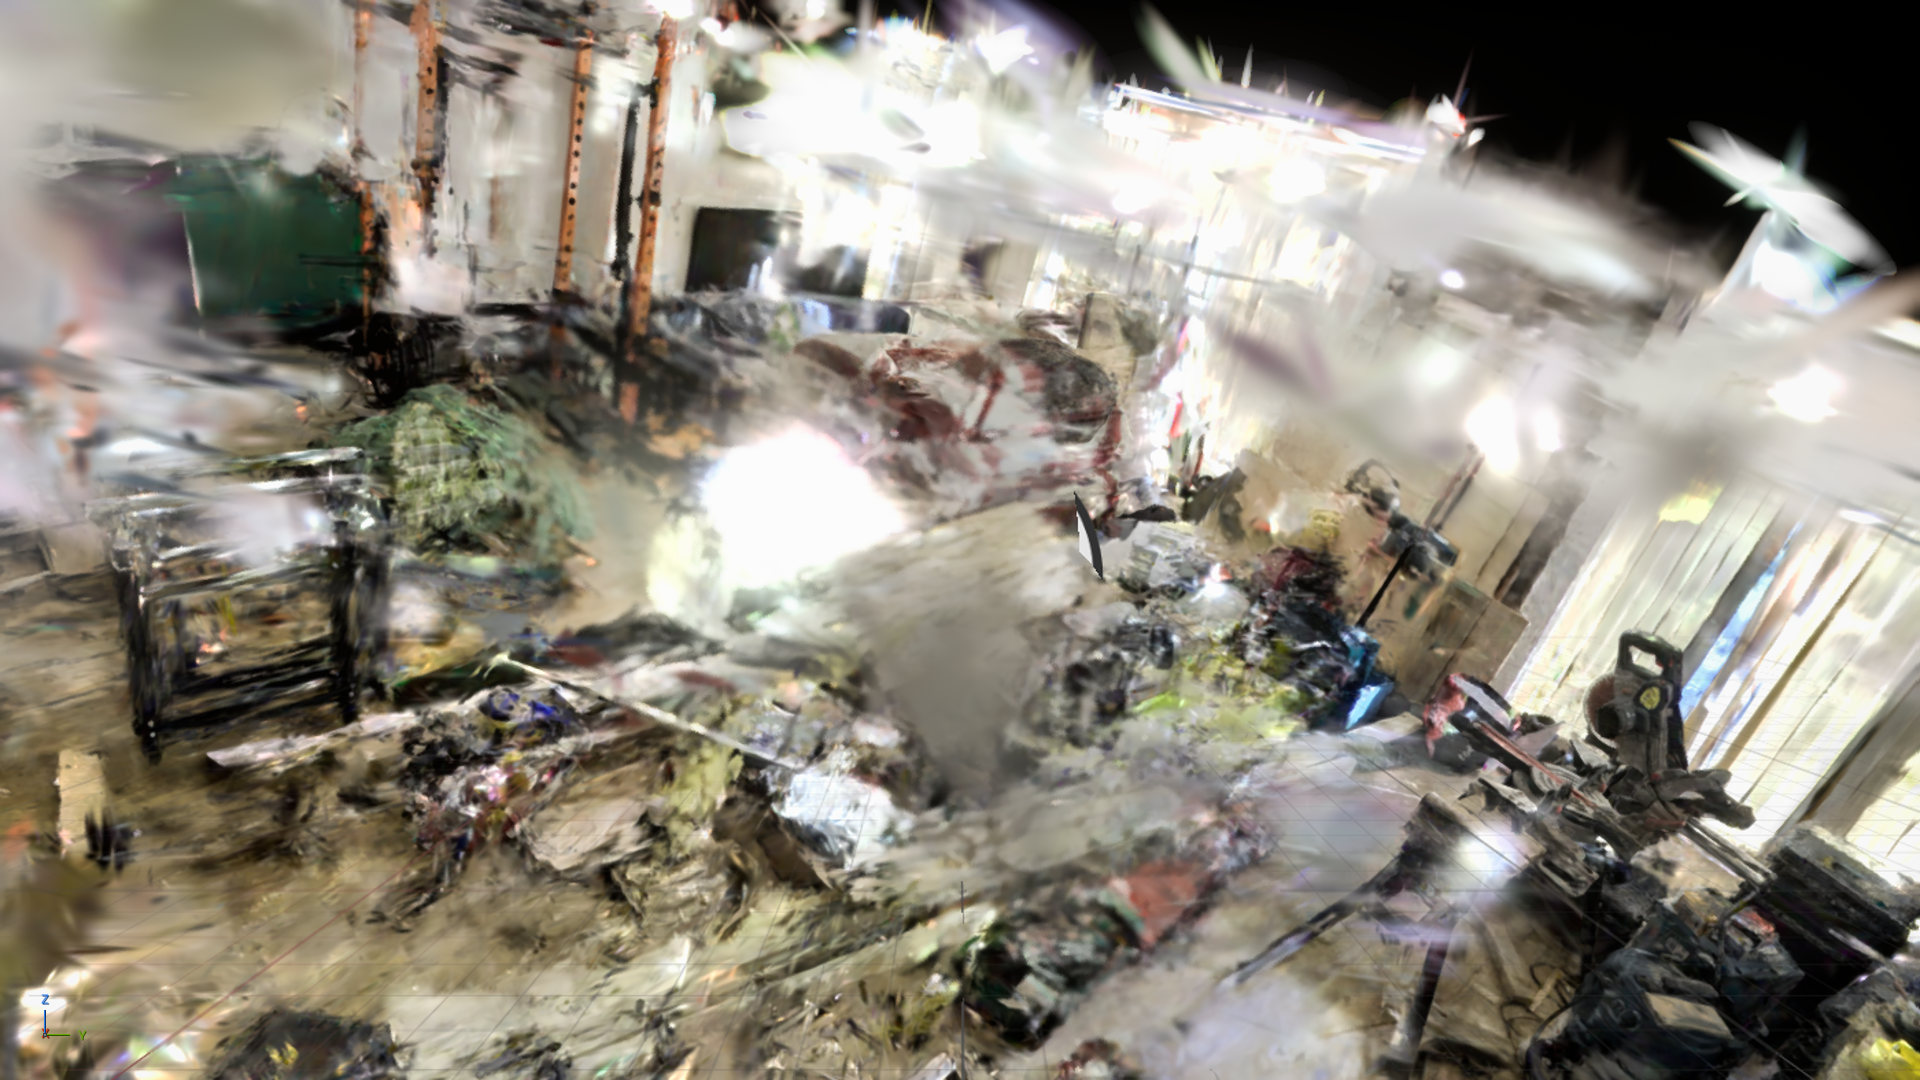
\includegraphics[width=\textwidth]{figures/nanogs_room_splat.png}
  \caption{%
    \textbf{Dreamlab room — NanoGS real-Gaussian splat render (canonical hero).}
    The LichtFeld-native \texttt{splat\_30000.ply}, cleaned via SuperSplat and
    loaded into the NanoGS\,(MIT) UE\,5.8 plugin, rendered at 1920$\times$1080.
    This replaces the earlier LiDAR point-cloud workaround and constitutes
    campaign step\,3: lean-on-LichtFeld native output for the room representation.
    Motion-blur softness in the source splat reflects the dreamlab capture
    constraint (MUSIQ $\approx$ 31); recapture at 4\,K\,/\,short shutter is the
    ceiling lever, not a pipeline limitation.
  }
  \label{fig:nanogs_room}
\end{figure}

% ──────────────────────────────────────────────────────────────────────────────
% 5. Fully integrated UE 5.8 scene
% ──────────────────────────────────────────────────────────────────────────────
\begin{figure}[htbp]
  \centering
  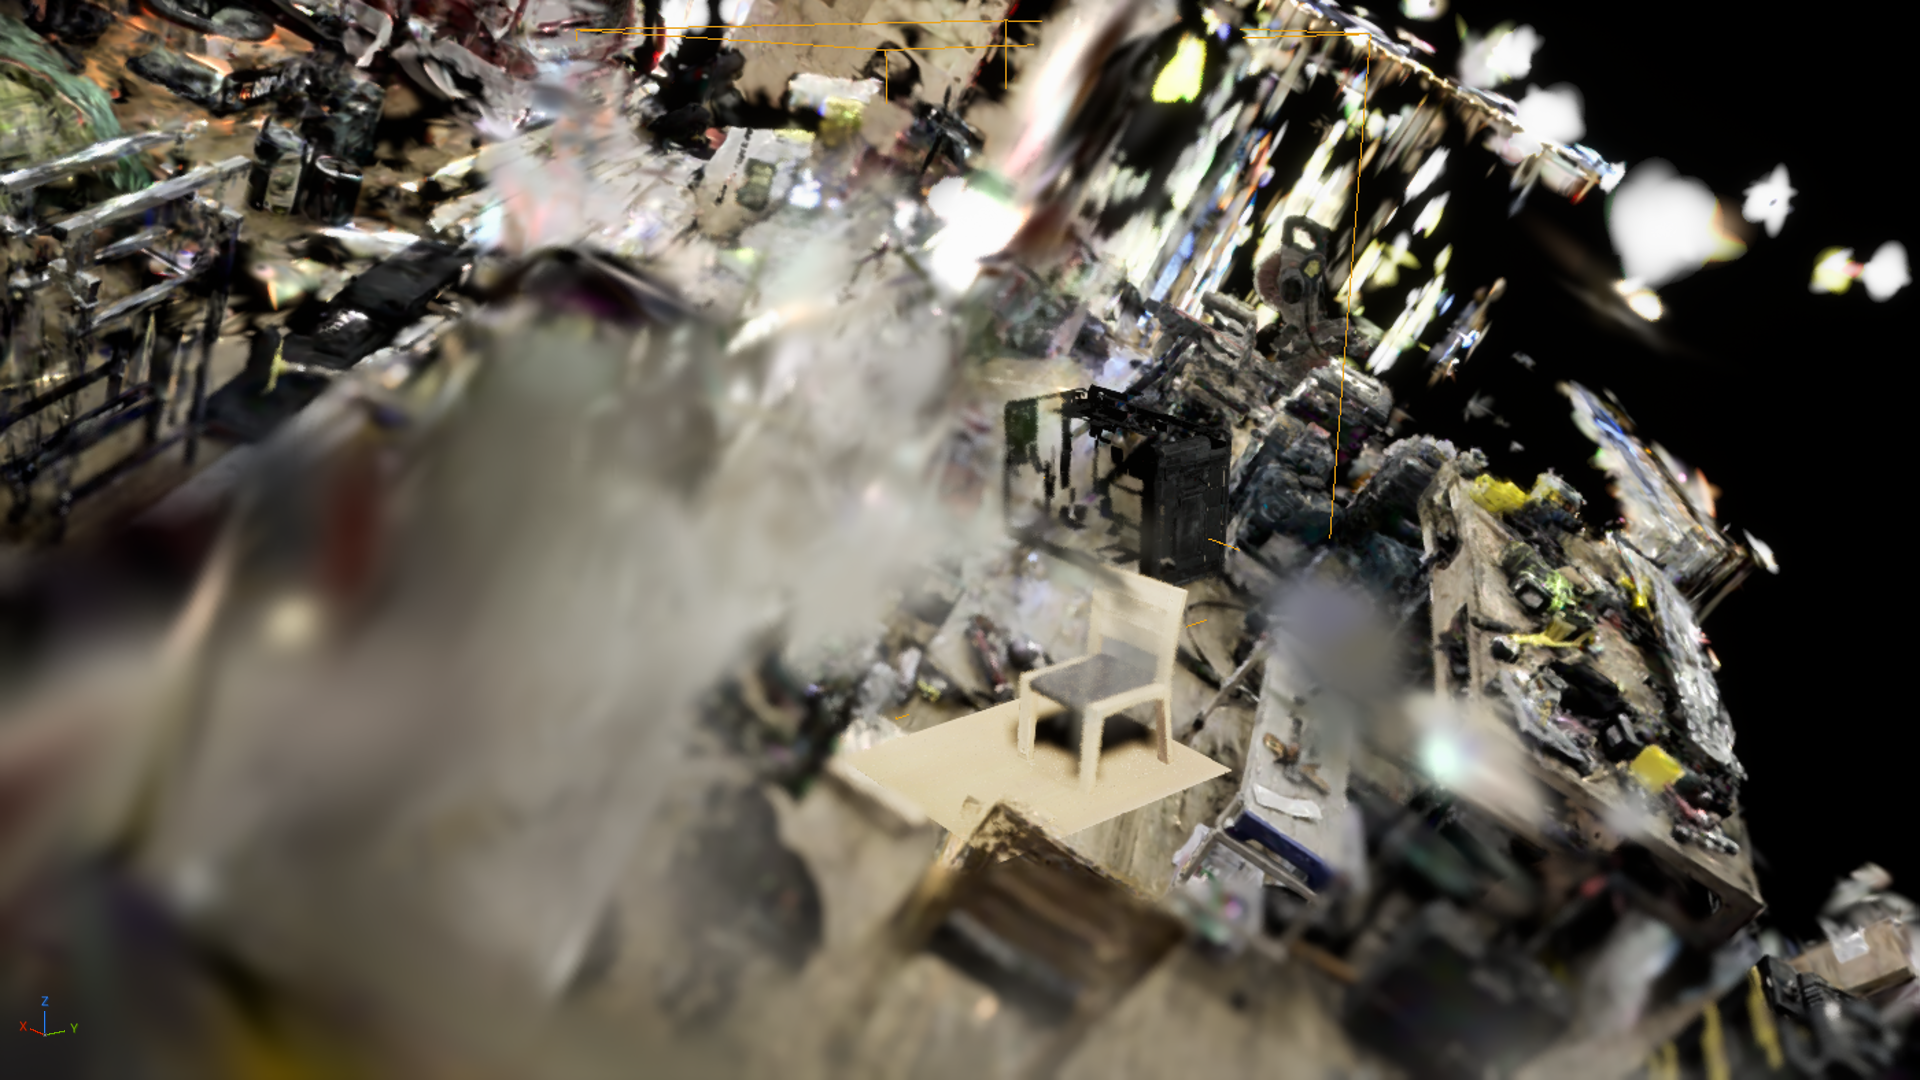
\includegraphics[width=\textwidth]{figures/scene_integrated.png}
  \caption{%
    \textbf{Integrated UE\,5.8 scene — room splat with placed TRELLIS.2 object FBXs.}
    The assembled deliverable: NanoGS splat room (hero representation) with
    chair, vacuum, and toolbox FBXs (TRELLIS.2 \texttt{hull\_e2e},
    prescaled via \texttt{blender\_prescale\_objects}) placed by
    \texttt{ue\_place\_prescaled}.
    Objects are Nanite game assets with baked PBR textures; the room splat
    renders real Gaussians.
    This image is the \emph{docs} canonical integrated-scene reference.
  }
  \label{fig:scene_integrated}
\end{figure}

% ──────────────────────────────────────────────────────────────────────────────
% 6. TRELLIS.2 object turnaround sheet (chair)
% ──────────────────────────────────────────────────────────────────────────────
\begin{figure}[htbp]
  \centering
  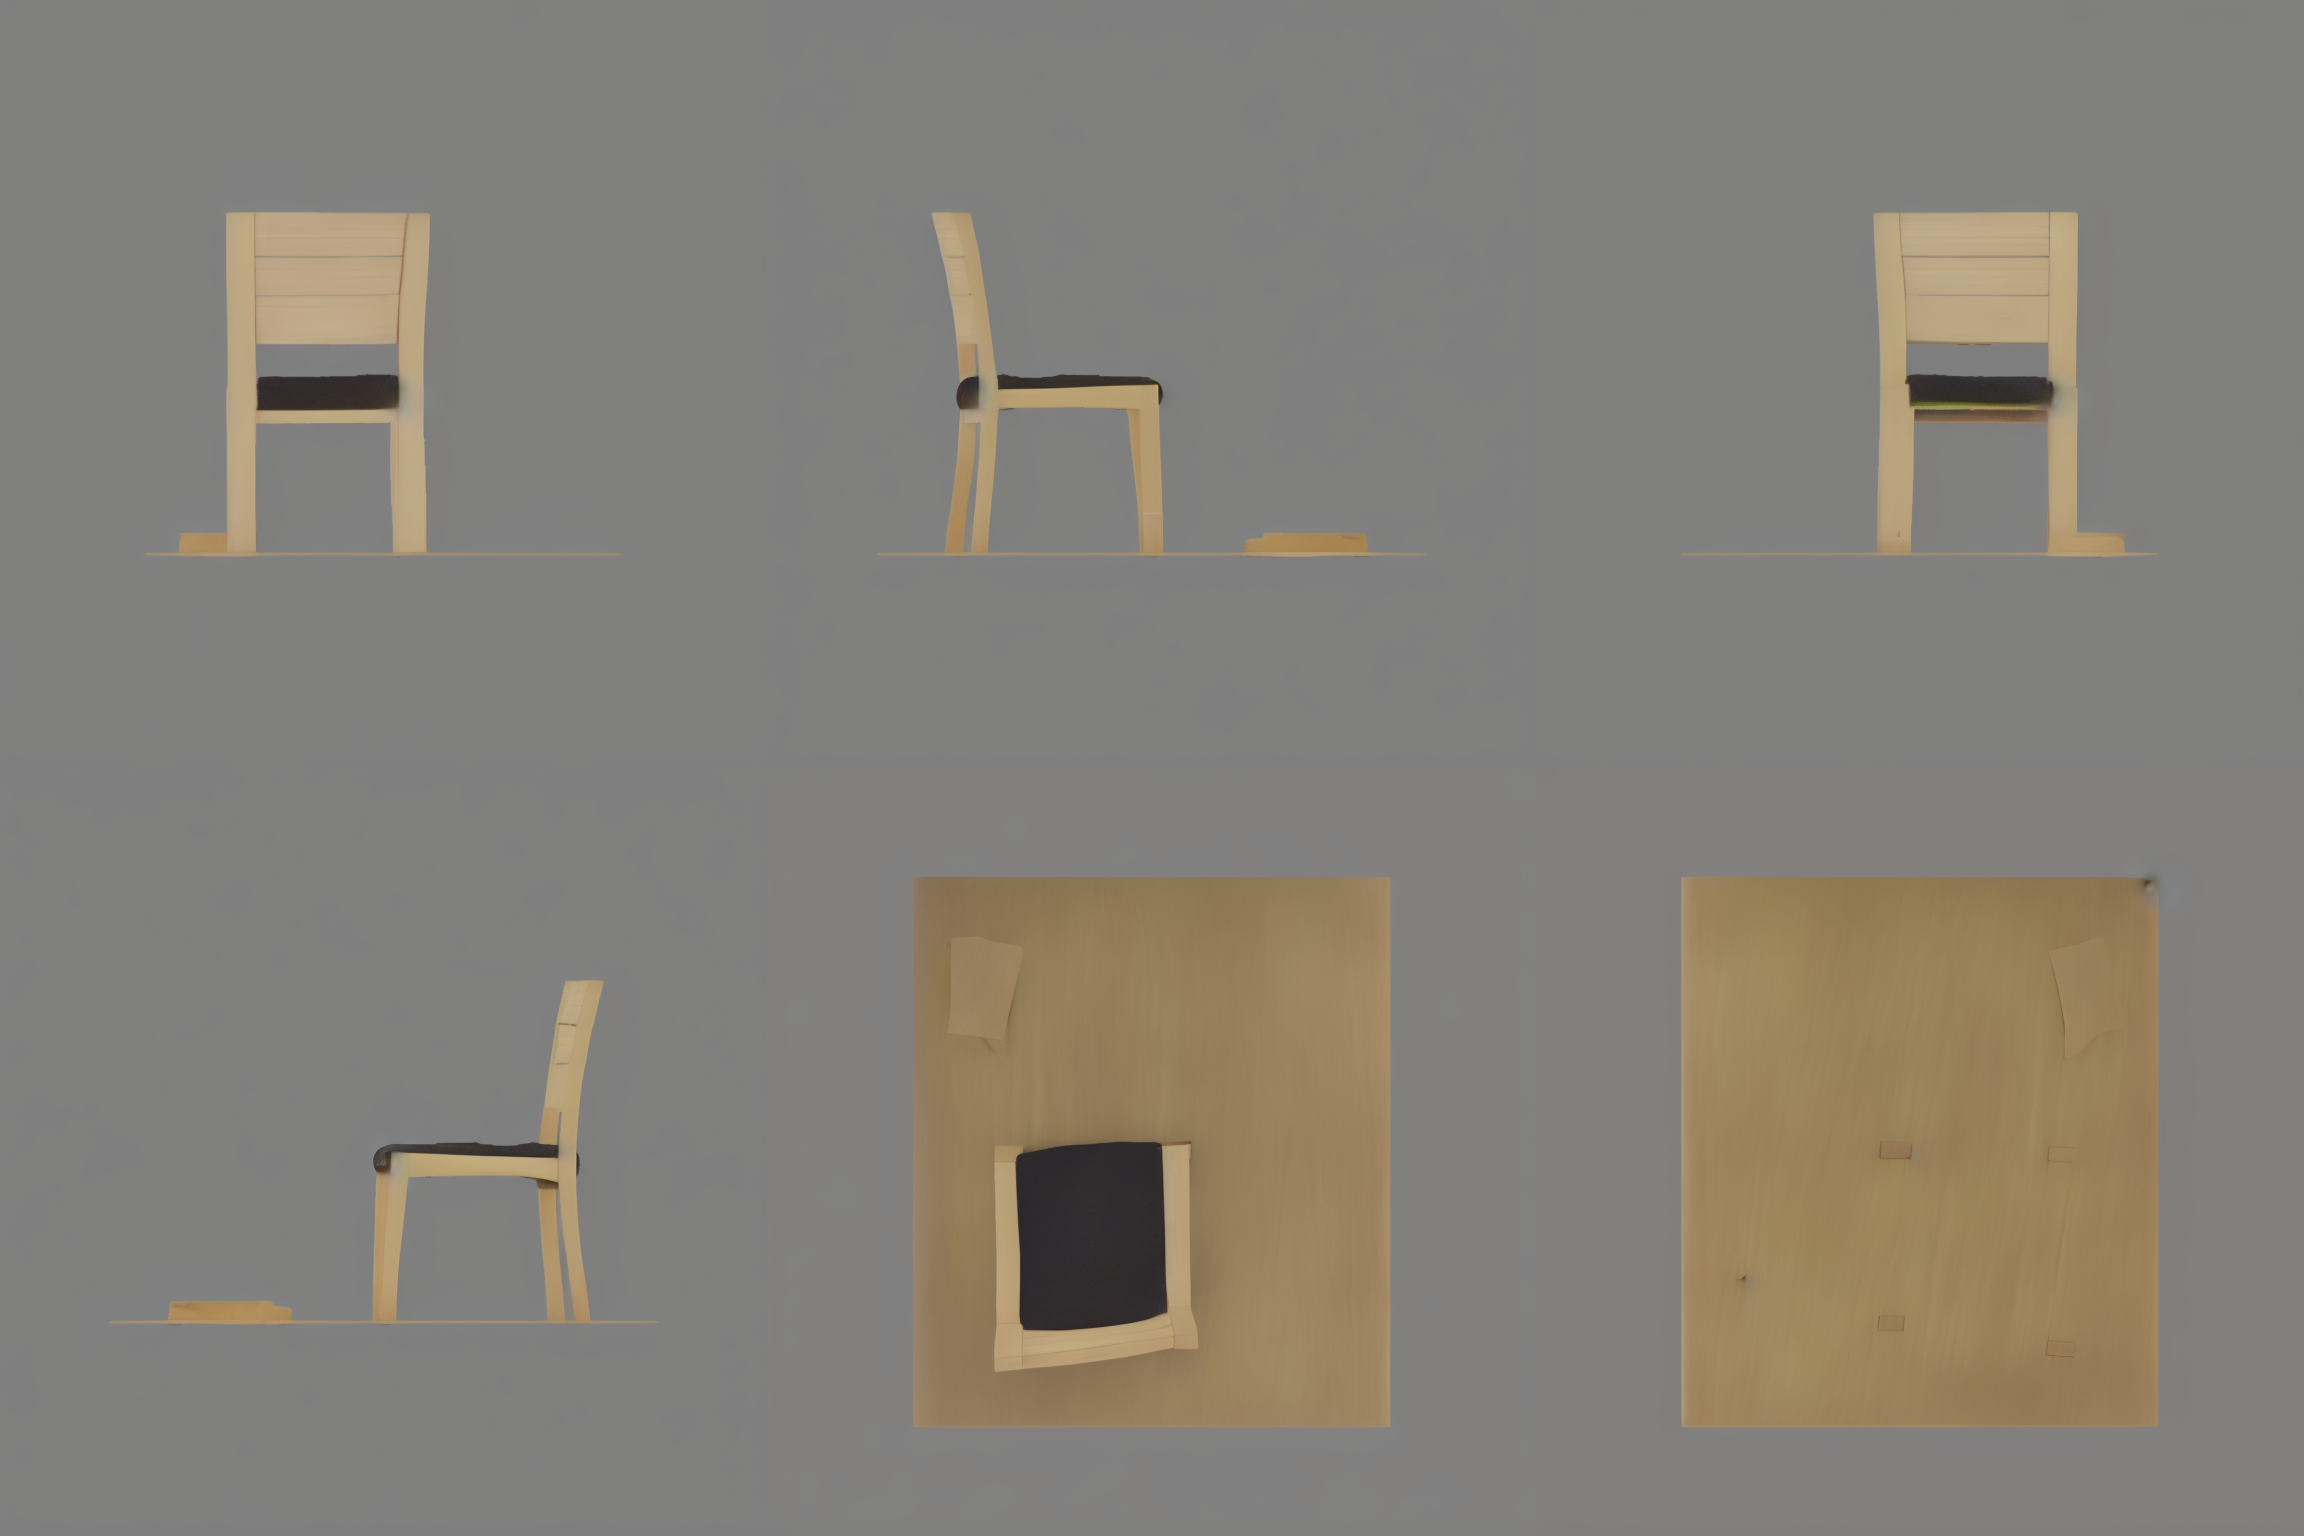
\includegraphics[width=\textwidth]{figures/chair_turnaround_sheet.png}
  \caption{%
    \textbf{TRELLIS.2 object reconstruction — chair turnaround sheet.}
    Multi-view orbit render of the textured GLB mesh produced by the
    \texttt{hull\_e2e} workflow: per-object SAM3 PLY crop $\to$ FLUX.2-dev
    view-inpainting $\to$ TRELLIS.2-4B mesh $\to$ PBR-baked GLB $\to$ FBX
    (Nanite game asset).
    The chair is rated \emph{good}; vacuum and toolbox likewise passed
    the object reconstruction gate (4/8 objects in this batch).
    Resolution: 2304$\times$1536.
  }
  \label{fig:objects}
\end{figure}

% ──────────────────────────────────────────────────────────────────────────────
% 7. CoMe-TSDF mesh in UE (baseline mesh deliverable)
% ──────────────────────────────────────────────────────────────────────────────
\begin{figure}[htbp]
  \centering
  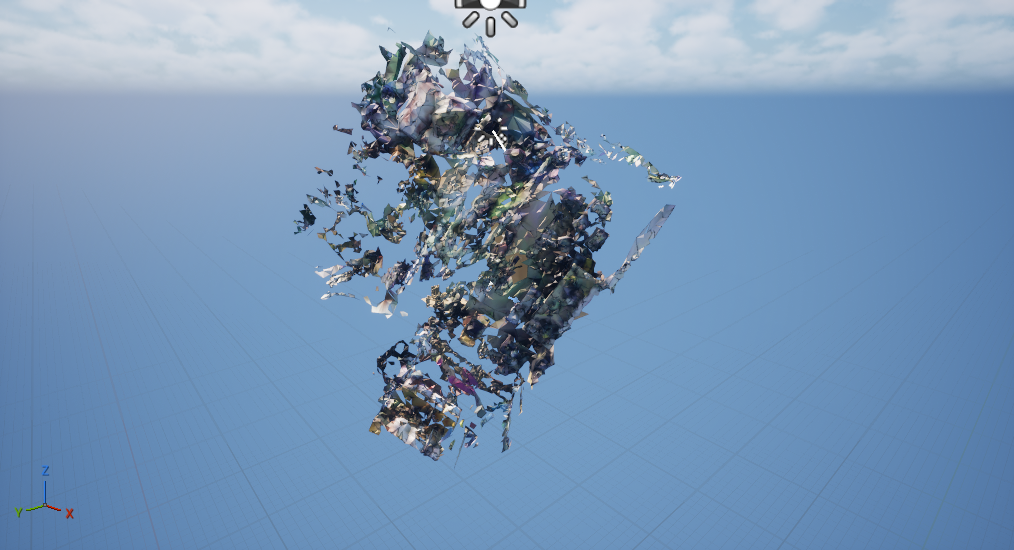
\includegraphics[width=\textwidth]{figures/ue_come_final.png}
  \caption{%
    \textbf{CoMe-TSDF room mesh game asset in UE\,5.8 (baseline mesh deliverable).}
    The scene-mesh branch: CoMe legacy \texttt{ScalableTSDFVolume} extraction,
    \texttt{mesh\_cleaner} (smooth=0, edge-length + connected-component cleanup),
    xatlas bake (\texttt{bake\_from\_vertex\_colors}), \texttt{blender\_obj\_to\_fbx},
    imported as a Nanite mesh.
    Characteristic TSDF blockiness on flat walls is visible; this image
    motivates the re-spine to NanoGS as the default room representation for
    blur-limited captures.
    Resolution: 1014$\times$550.
  }
  \label{fig:ue_come}
\end{figure}

% ──────────────────────────────────────────────────────────────────────────────
% 8. NanoGS splat render (1920×1080 B-view)
% ──────────────────────────────────────────────────────────────────────────────
\begin{figure}[htbp]
  \centering
  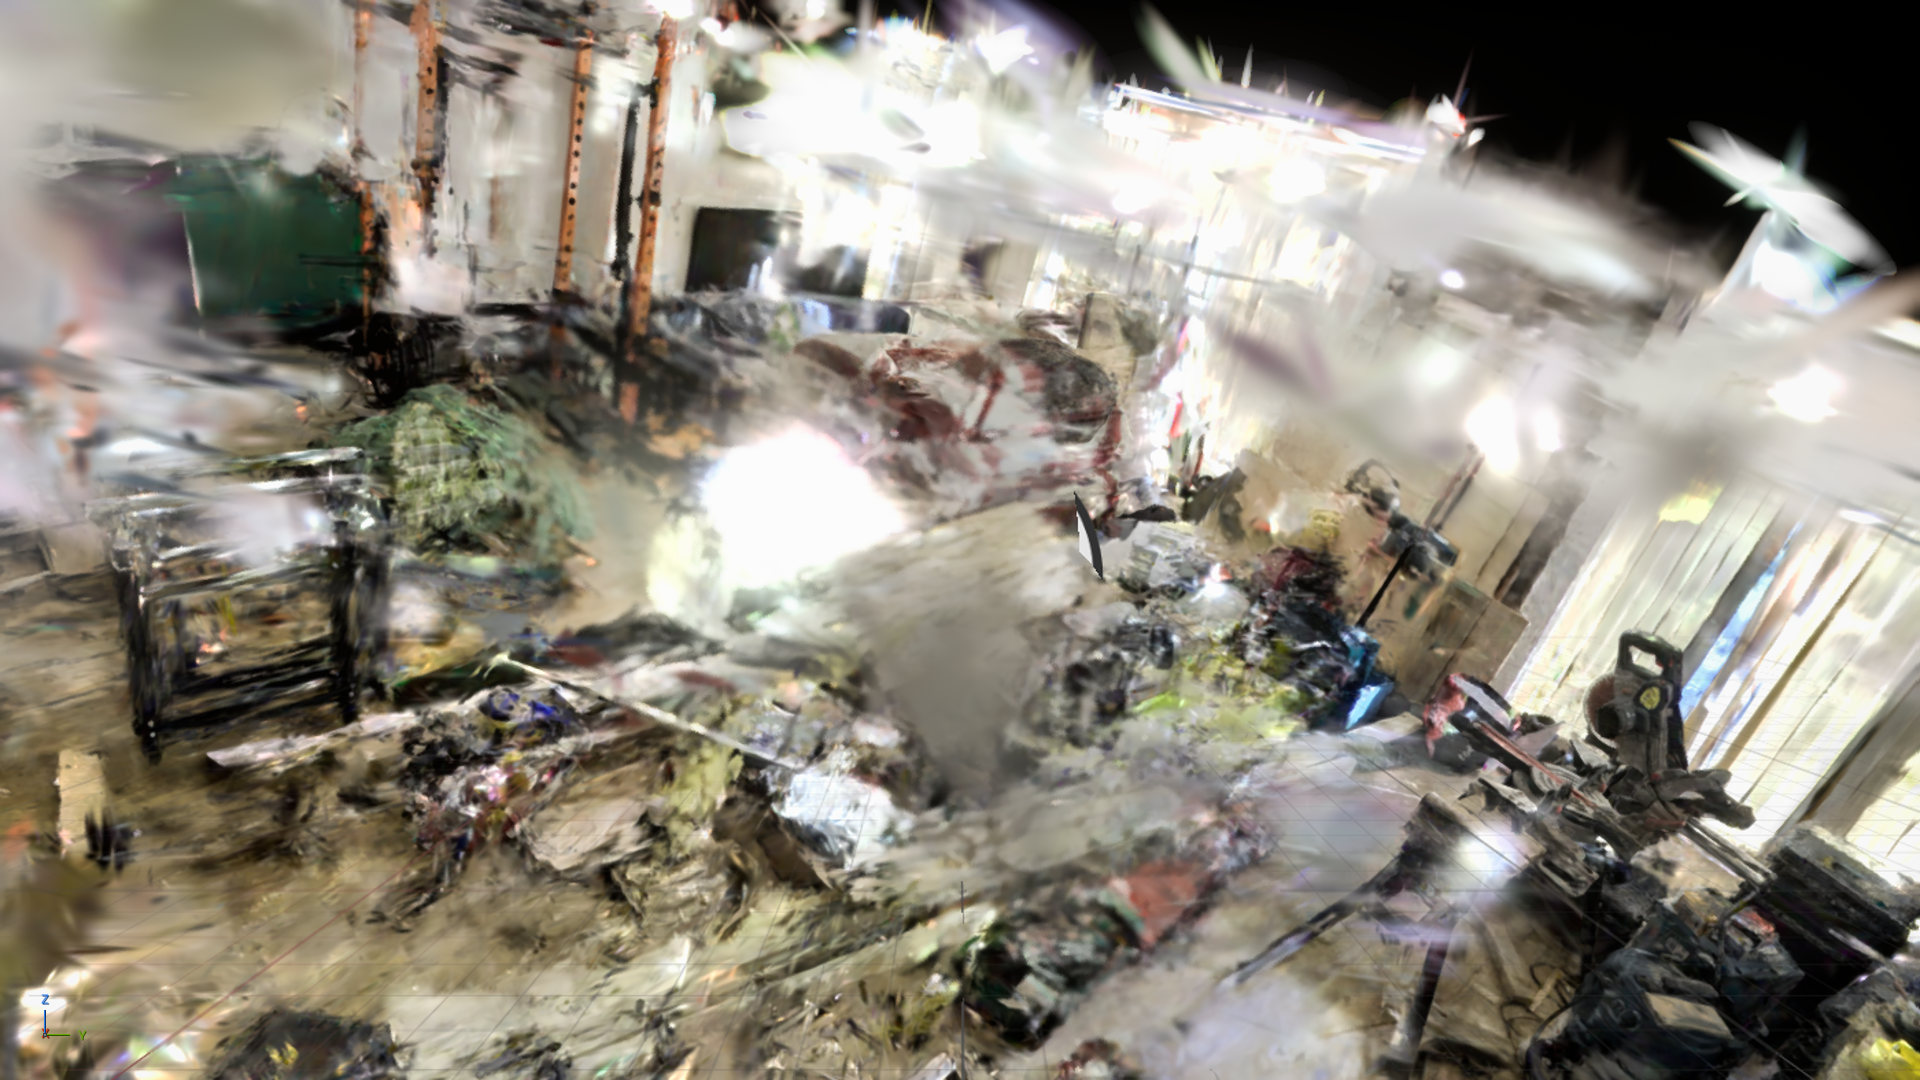
\includegraphics[width=\textwidth]{figures/ue_nanogs_room_B.png}
  \caption{%
    \textbf{NanoGS real-Gaussian splat in UE\,5.8 — interior view (B).}
    Second viewpoint of the NanoGS splat room, demonstrating depth and
    parallax of real Gaussian rendering at 1920$\times$1080.
    Comparison with Figure~\ref{fig:ue_come} illustrates the quality
    improvement of splat-hero over TSDF mesh for a motion-blur-limited
    capture: the splat faithfully preserves captured radiance;
    the mesh introduces geometric artefacts irrelevant to the capture.
  }
  \label{fig:ue_nanogs}
\end{figure}

% ──────────────────────────────────────────────────────────────────────────────
% 9. Hero perspective render (room + placed objects)
% ──────────────────────────────────────────────────────────────────────────────
\begin{figure}[htbp]
  \centering
  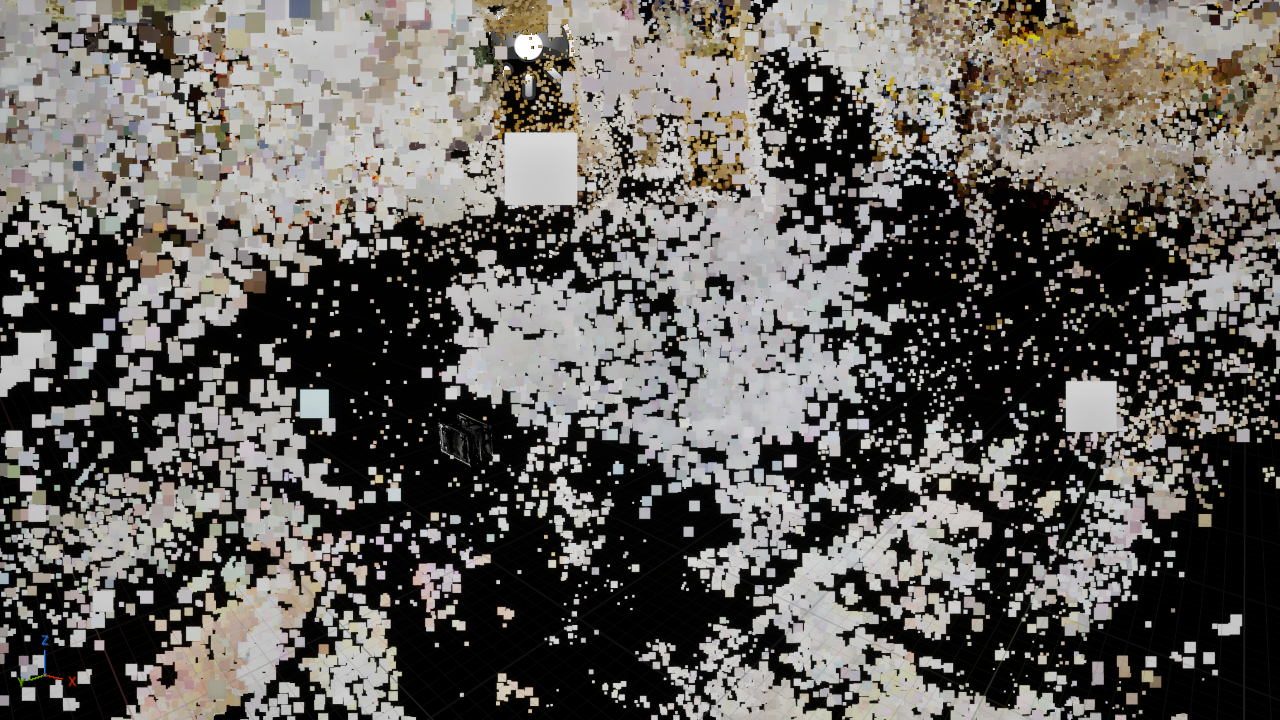
\includegraphics[width=\textwidth]{figures/ue_final_hero.png}
  \caption{%
    \textbf{Hero perspective render — dreamlab room with placed object FBXs.}
    A cinematic view of the assembled UE\,5.8 scene from the validated
    end-to-end run (2026-06-22): TSDF-mesh room (CoMe, pre-NanoGS re-spine)
    with TRELLIS.2 object FBXs placed by \texttt{ue\_place\_prescaled}.
    Resolution: 1280$\times$720.
    Serves as the primary before/after reference for evaluating the
    NanoGS re-spine (Figure~\ref{fig:nanogs_room}).
  }
  \label{fig:ue_hero}
\end{figure}

% ──────────────────────────────────────────────────────────────────────────────
% 10. Overhead dollhouse view
% ──────────────────────────────────────────────────────────────────────────────
\begin{figure}[htbp]
  \centering
  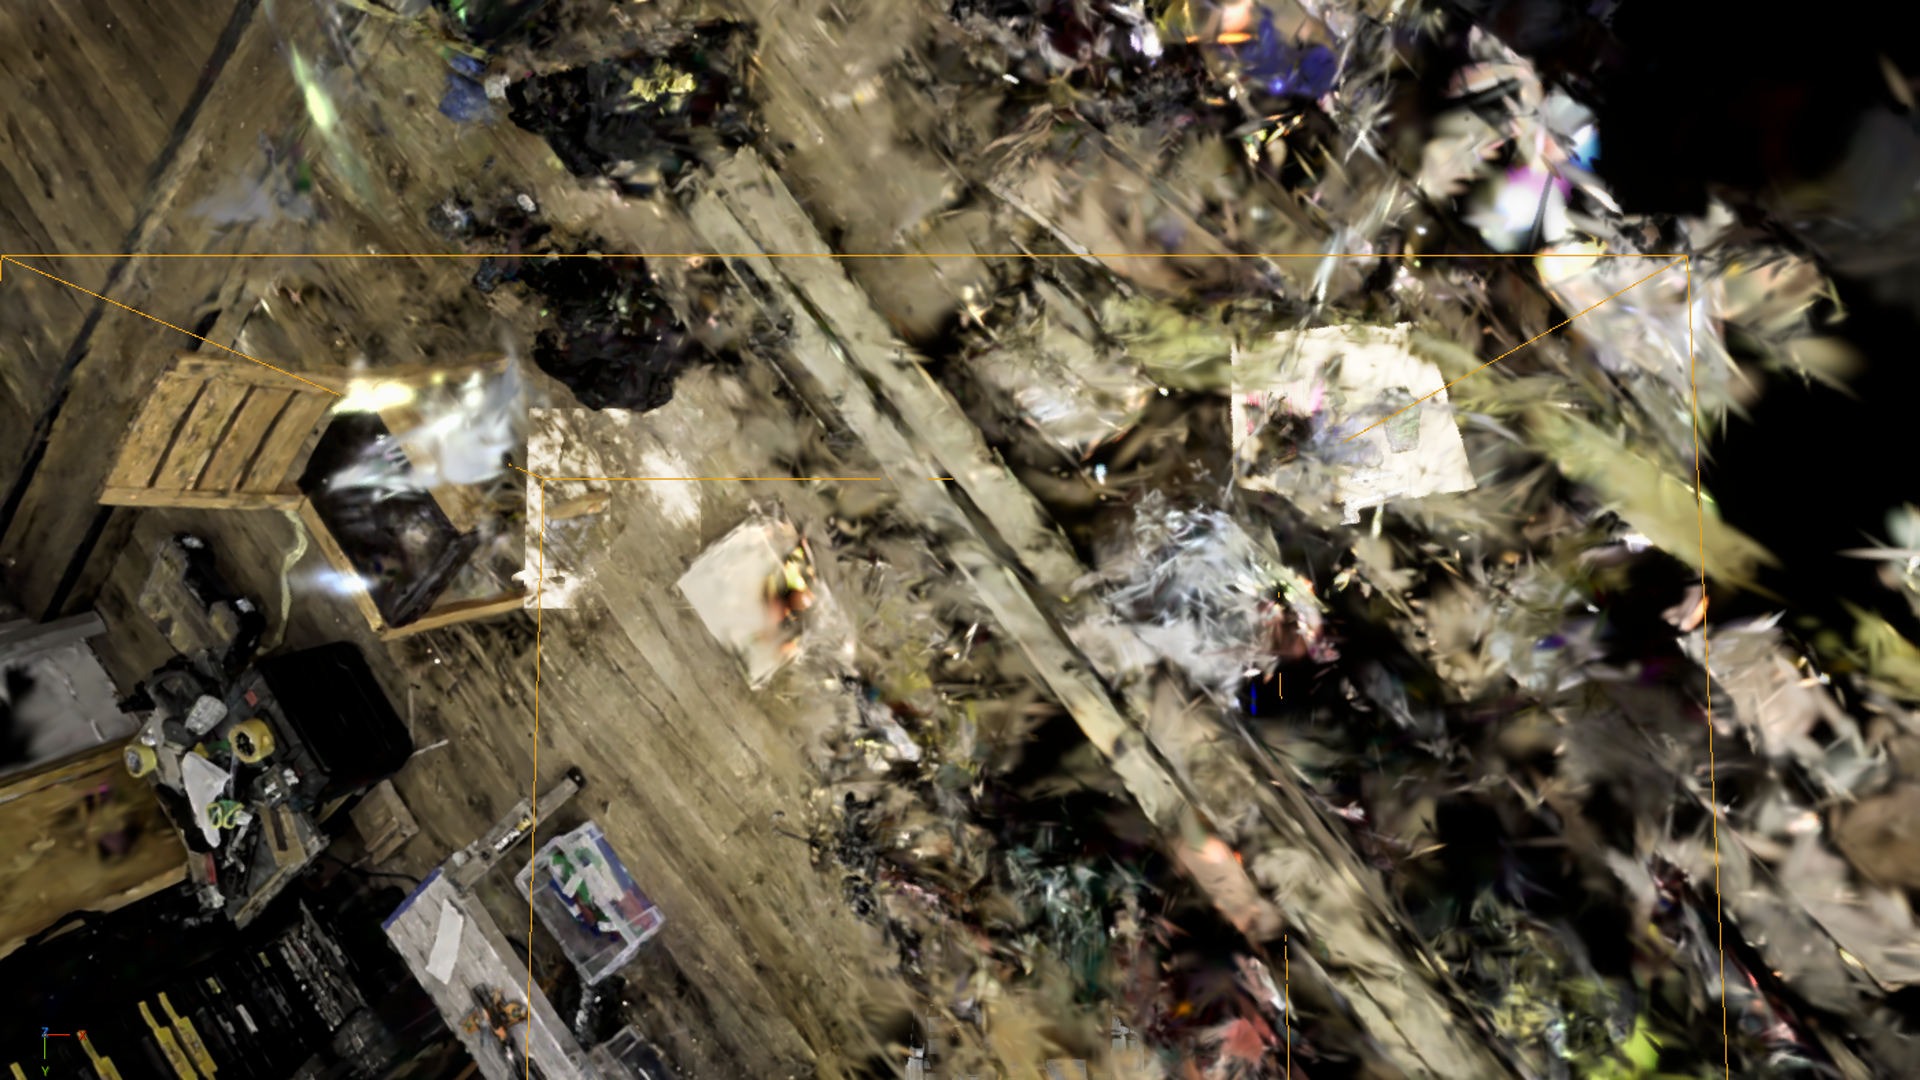
\includegraphics[width=\textwidth]{figures/ue_integrated_dollhouse.png}
  \caption{%
    \textbf{Overhead dollhouse view — integrated UE\,5.8 scene layout.}
    Top-down perspective revealing object placement, room geometry, and
    spatial relationships of the dreamlab scene.
    The dollhouse view is the standard QA checkpoint for scale fidelity
    and object-in-room alignment after \texttt{ue\_place\_prescaled}
    prescaling.
    Resolution: 1920$\times$1080.
  }
  \label{fig:ue_dollhouse}
\end{figure}

% Assumes \graphicspath{{figures/}} is set in the preamble (relative to report/v5/).
%
% Labels (for \ref / \autoref):
%   fig:router           — capture-adaptive router flowchart
%   fig:component_menu   — component-menu status flowchart
%   fig:architecture     — system architecture (container topology)
%   fig:nanogs_room      — NanoGS real-Gaussian splat render (canonical room hero)
%   fig:scene_integrated — fully integrated UE 5.8 scene (room + objects)
%   fig:objects          — TRELLIS.2 object turnaround sheet (chair)
%   fig:ue_come          — CoMe-TSDF mesh game asset in UE (baseline mesh)
%   fig:ue_nanogs        — NanoGS splat render (dreamlab room, 1920x1080)
%   fig:ue_hero          — Hero perspective render (room + placed objects)
%   fig:ue_dollhouse     — Overhead dollhouse view of integrated UE scene

% ──────────────────────────────────────────────────────────────────────────────
% 1. Capture-adaptive router
% ──────────────────────────────────────────────────────────────────────────────
\begin{figure}[htbp]
  \centering
  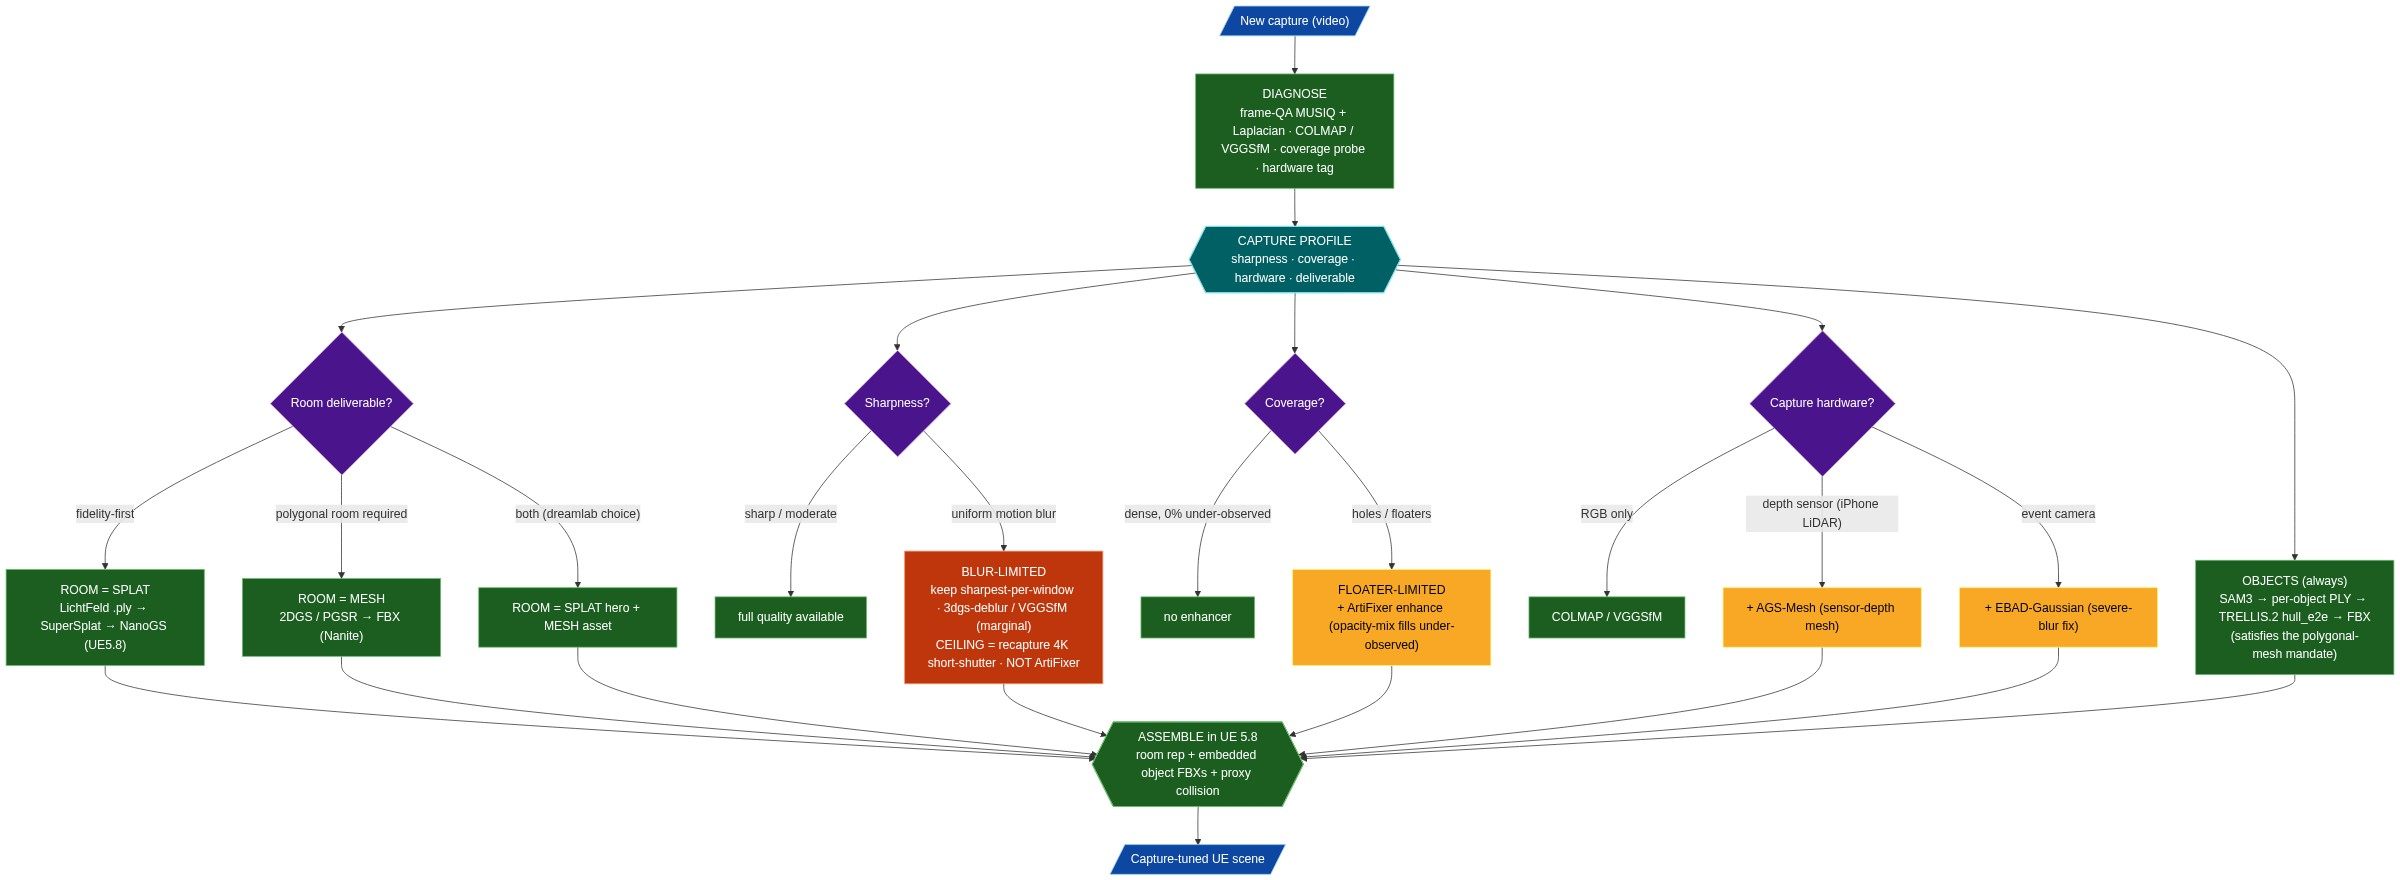
\includegraphics[width=\textwidth]{figures/router.jpg}
  \caption{%
    \textbf{Capture-adaptive router.}
    The pipeline diagnoses each new capture on four axes
    (sharpness via MUSIQ + full-resolution Laplacian, coverage via occupancy probe,
    available hardware, and deliverable type) and selects the configuration that
    fits the bottleneck.
    Green nodes are validated keepers; orange nodes are
    capture-conditional options; red nodes are blur-limited warnings.
    The dreamlab capture routes to Opt\,4 (splat hero + mesh asset + TRELLIS.2 objects)
    with a recapture flag as the quality ceiling.
  }
  \label{fig:router}
\end{figure}

% ──────────────────────────────────────────────────────────────────────────────
% 2. Component-menu flowchart
% ──────────────────────────────────────────────────────────────────────────────
\begin{figure}[htbp]
  \centering
  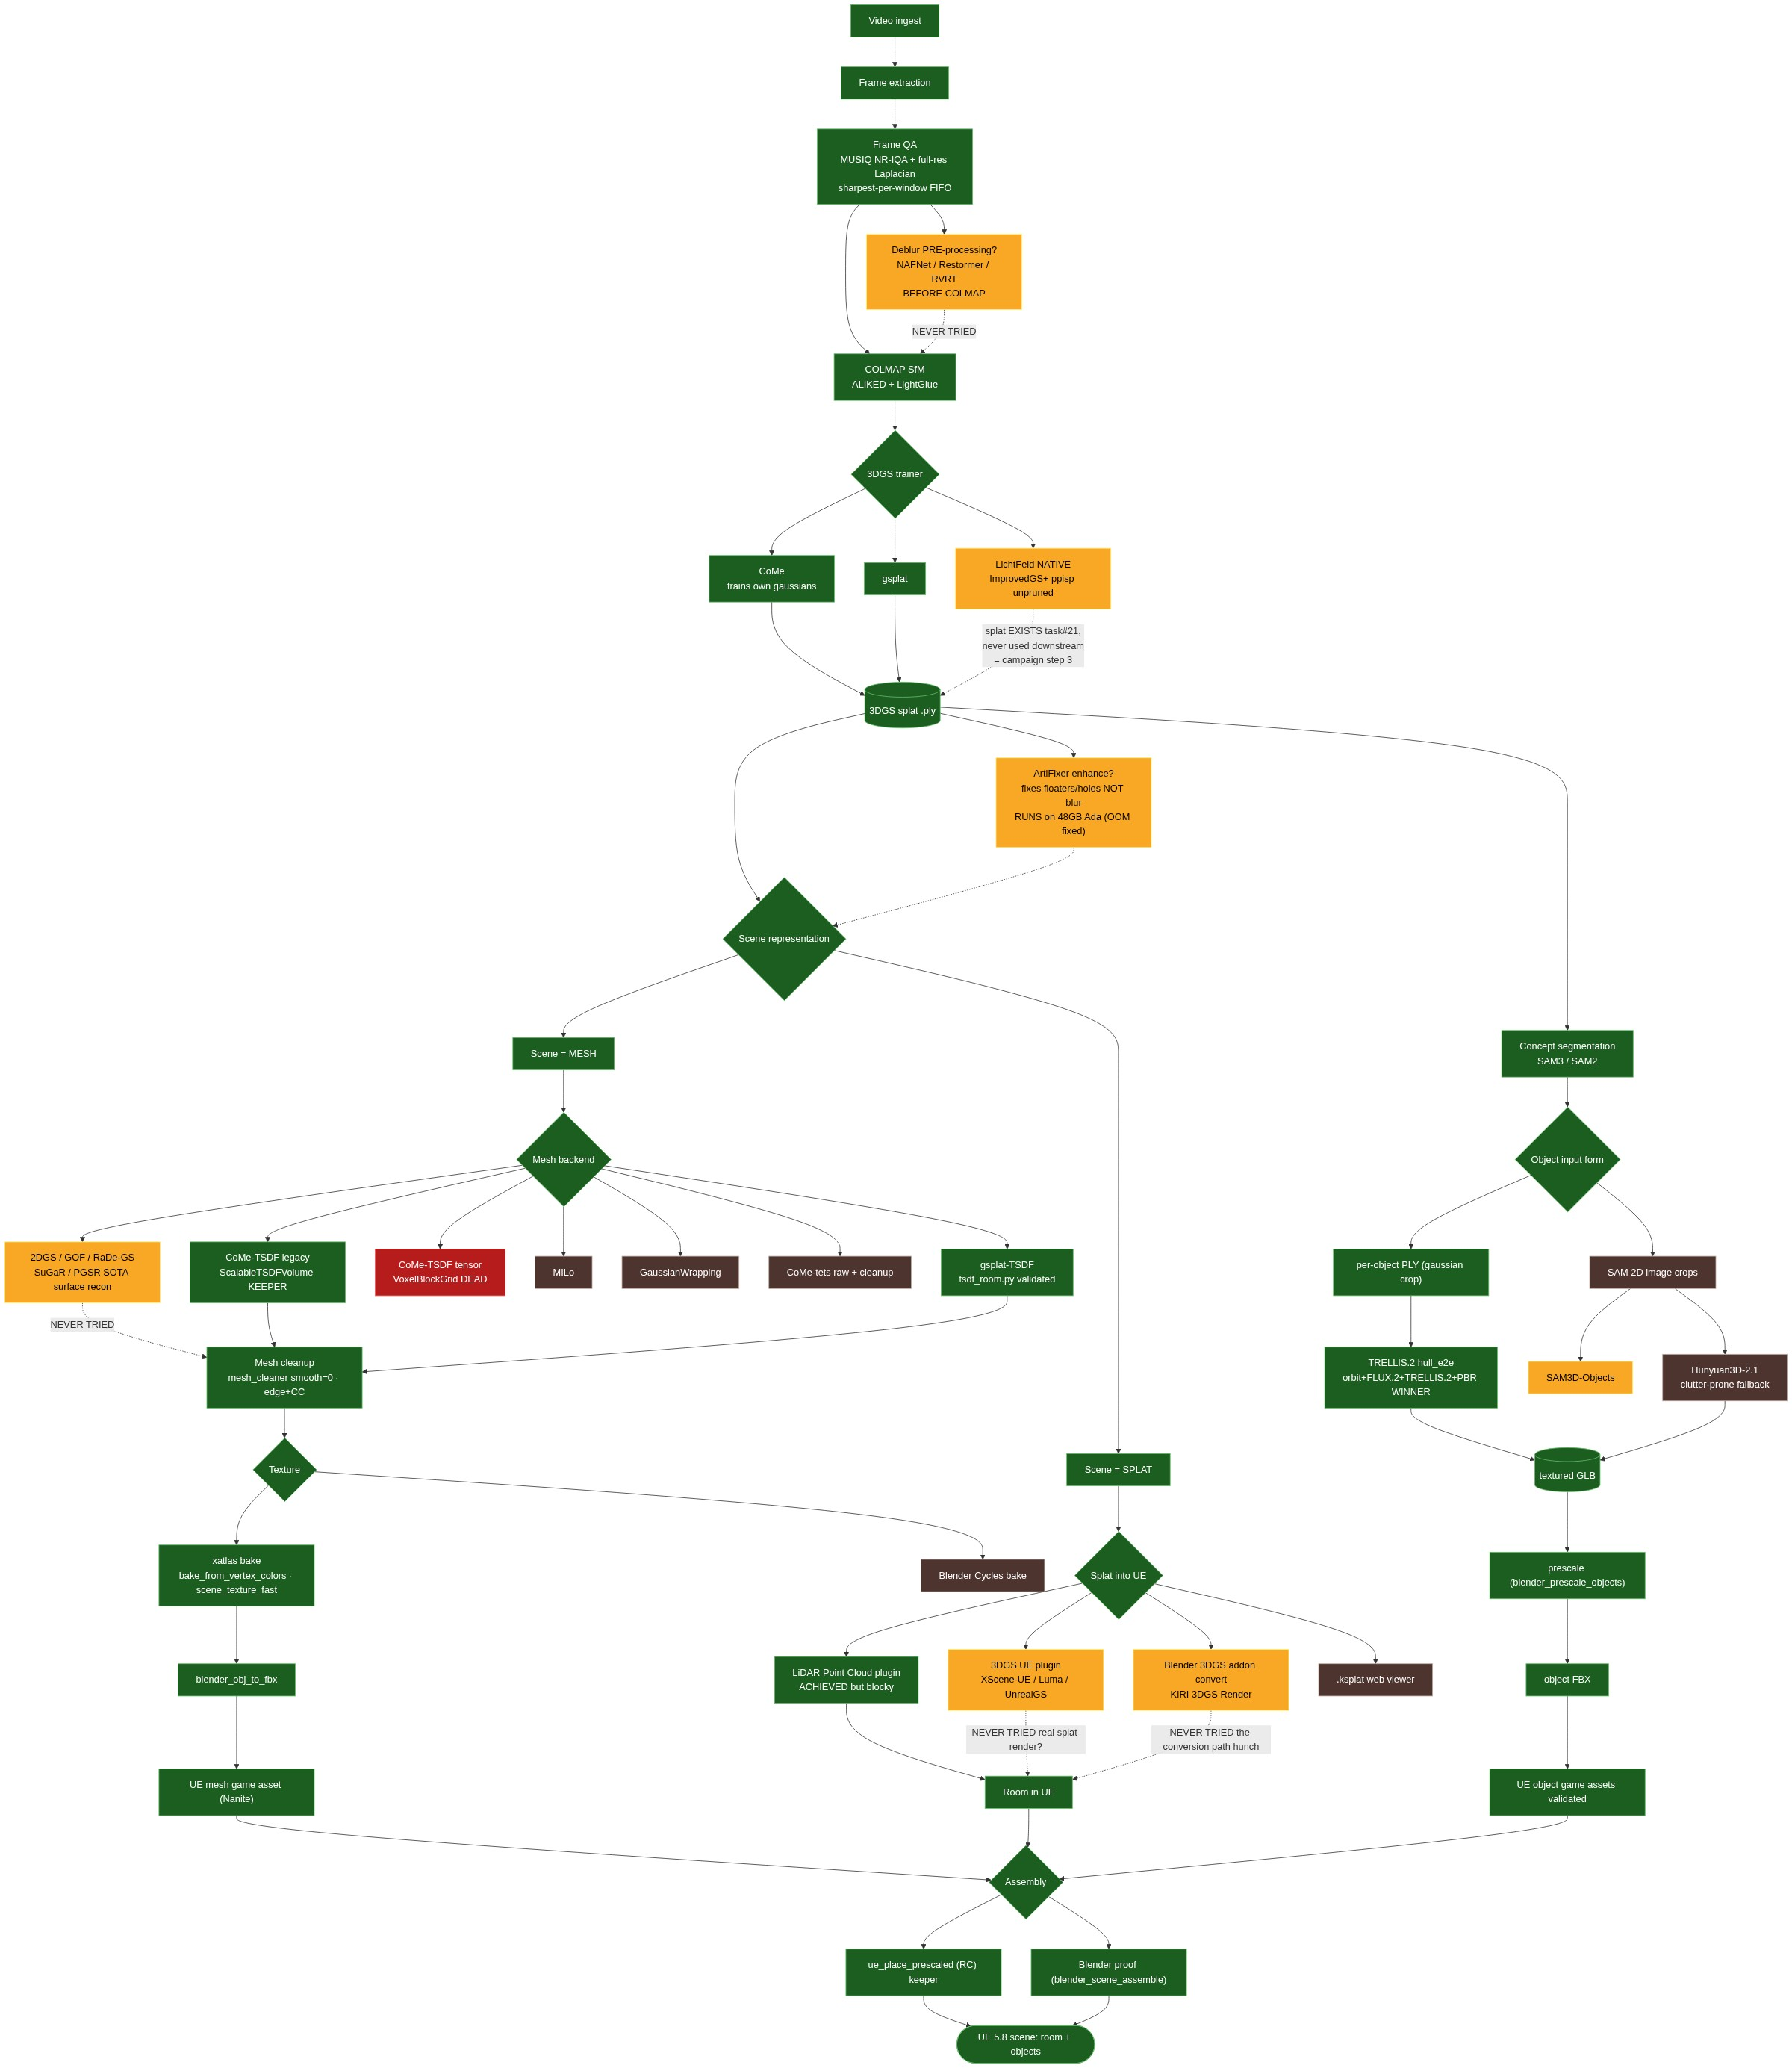
\includegraphics[width=\textwidth]{figures/component_menu.jpg}
  \caption{%
    \textbf{Full component-menu status chart (validated 2026-06-25).}
    Every branch of the Vitrine toolkit from video ingest to UE\,5.8 delivery.
    Colour coding: \emph{green} = validated keeper in active use;
    \emph{brown} = exercised but subordinate / fallback;
    \emph{red} = tried and abandoned;
    \emph{yellow} = plausible, never run.
    The chart is the canonical record of what has and has not been exercised;
    dashed arrows mark paths that remain open research items
    (SAM3D-Objects, BAD-Gaussians deblur, PGSR/2DGS surface reconstruction).
  }
  \label{fig:component_menu}
\end{figure}

% ──────────────────────────────────────────────────────────────────────────────
% 3. System architecture (container topology)
% ──────────────────────────────────────────────────────────────────────────────
\begin{figure}[htbp]
  \centering
  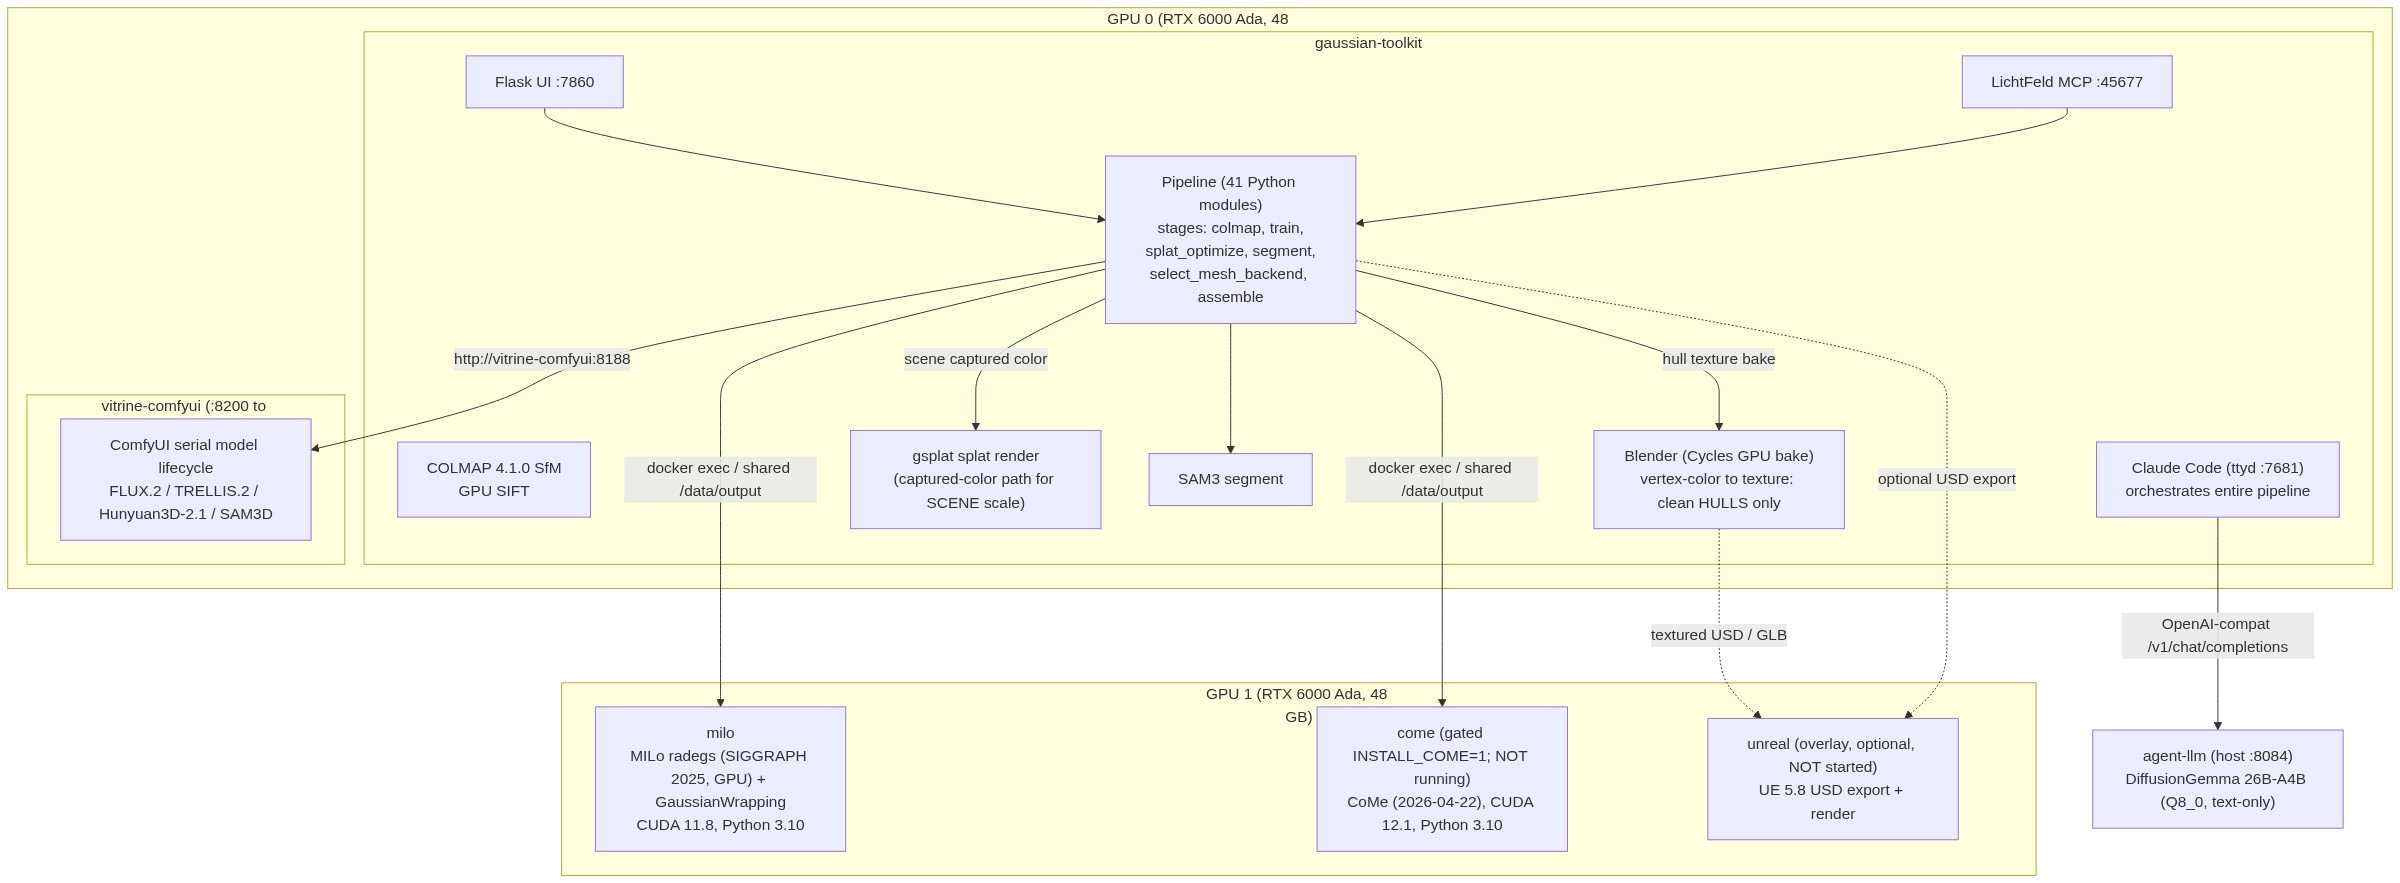
\includegraphics[width=\textwidth]{figures/architecture.jpg}
  \caption{%
    \textbf{Vitrine system architecture — Docker container topology.}
    Two RTX\,6000\,Ada GPUs (48\,GB each) host the six-container stack.
    GPU\,0 runs the \texttt{gaussian-toolkit} orchestrator (COLMAP, LichtFeld
    3DGS, SAM3, Flask\,UI, LichtFeld\,MCP on port\,45677) and
    \texttt{vitrine-comfyui} (FLUX.2\,/\,TRELLIS.2\,/\,Hunyuan3D-2.1, serial
    model lifecycle).
    GPU\,1 hosts the \texttt{milo} sidecar (MILo radegs, CUDA\,11.8) and the
    optional \texttt{come} (CoMe, CUDA\,12.1) and \texttt{unreal} (UE\,5.8)
    overlay containers.
    DiffusionGemma\,26B-A4B runs on the host at port\,8084 as the local text
    reasoner.
    All pipeline containers share \texttt{v2g-net}; the agentbox (Claude Code)
    reaches them via the shared \texttt{visionclaw\_network}.
  }
  \label{fig:architecture}
\end{figure}

% ──────────────────────────────────────────────────────────────────────────────
% 4. NanoGS room splat (docs canonical hero)
% ──────────────────────────────────────────────────────────────────────────────
\begin{figure}[htbp]
  \centering
  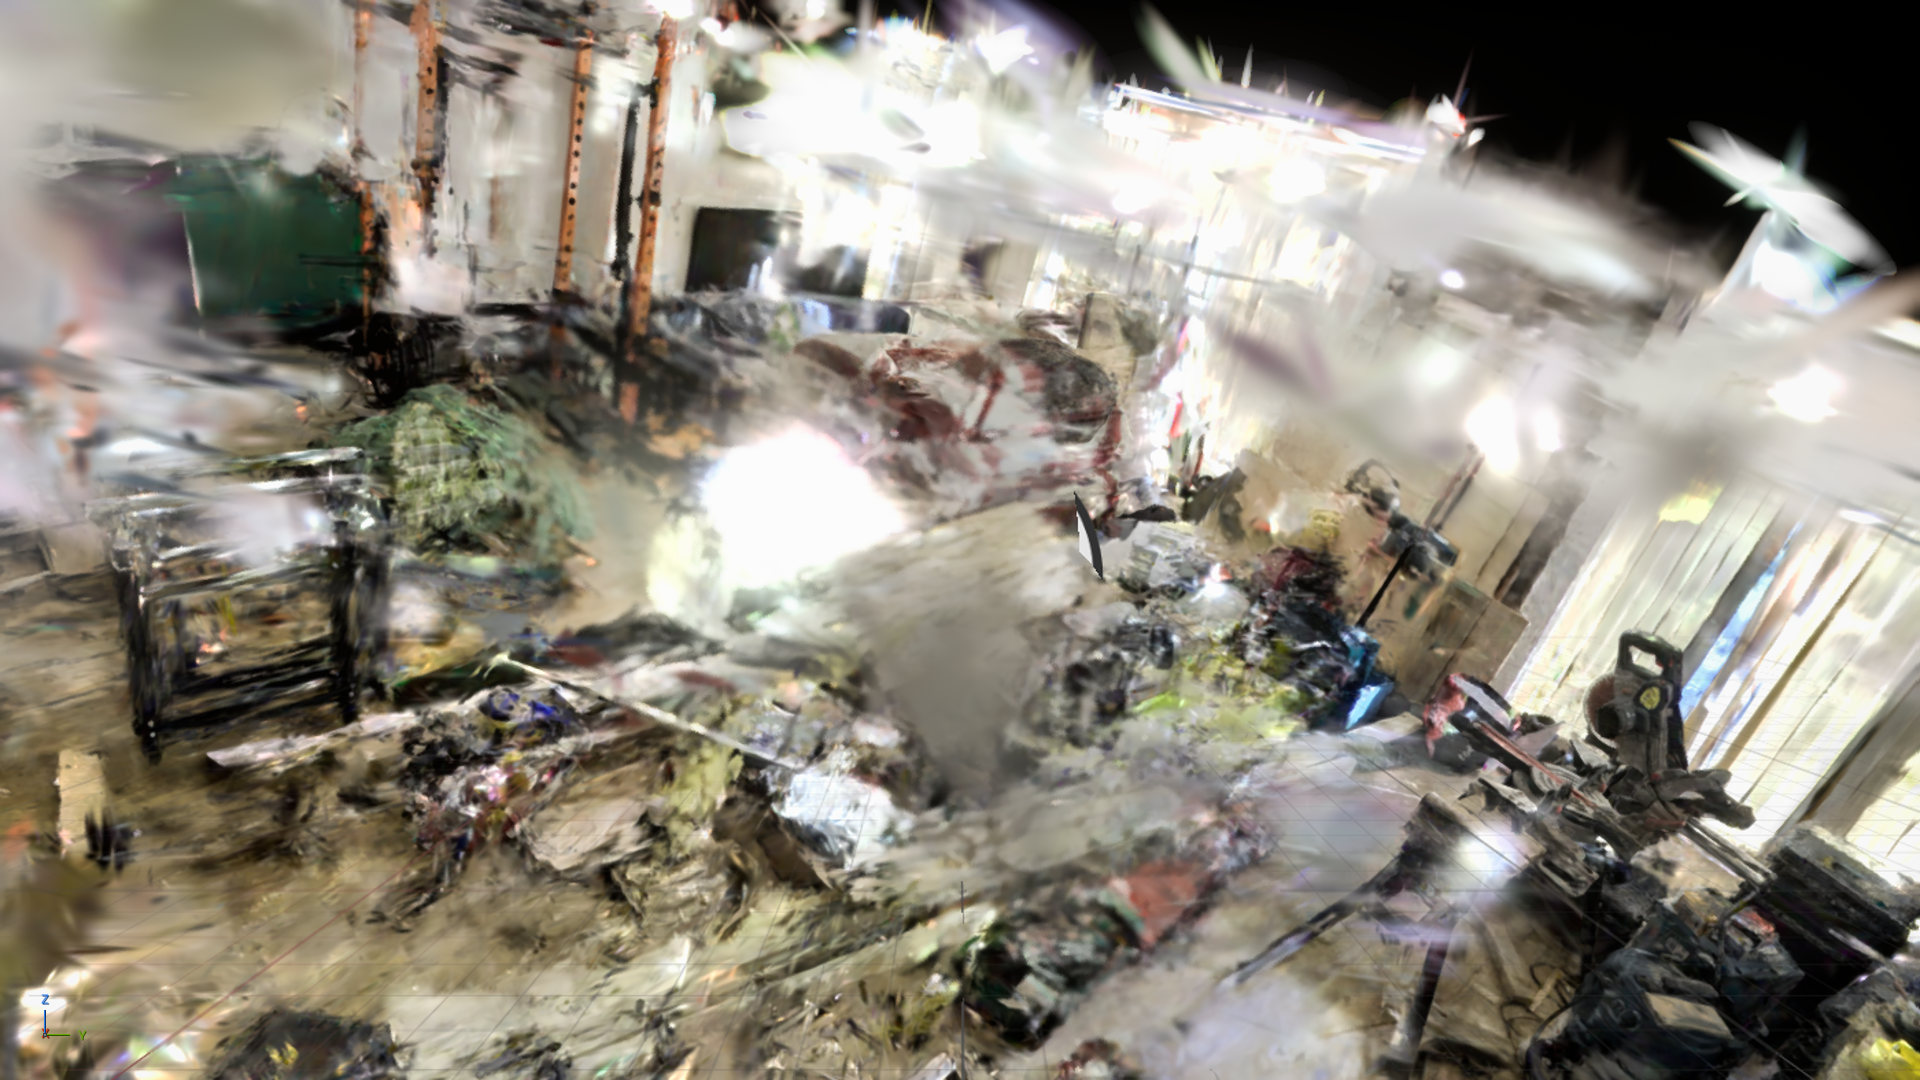
\includegraphics[width=\textwidth]{figures/nanogs_room_splat.png}
  \caption{%
    \textbf{Dreamlab room — NanoGS real-Gaussian splat render (canonical hero).}
    The LichtFeld-native \texttt{splat\_30000.ply}, cleaned via SuperSplat and
    loaded into the NanoGS\,(MIT) UE\,5.8 plugin, rendered at 1920$\times$1080.
    This replaces the earlier LiDAR point-cloud workaround and constitutes
    campaign step\,3: lean-on-LichtFeld native output for the room representation.
    Motion-blur softness in the source splat reflects the dreamlab capture
    constraint (MUSIQ $\approx$ 31); recapture at 4\,K\,/\,short shutter is the
    ceiling lever, not a pipeline limitation.
  }
  \label{fig:nanogs_room}
\end{figure}

% ──────────────────────────────────────────────────────────────────────────────
% 5. Fully integrated UE 5.8 scene
% ──────────────────────────────────────────────────────────────────────────────
\begin{figure}[htbp]
  \centering
  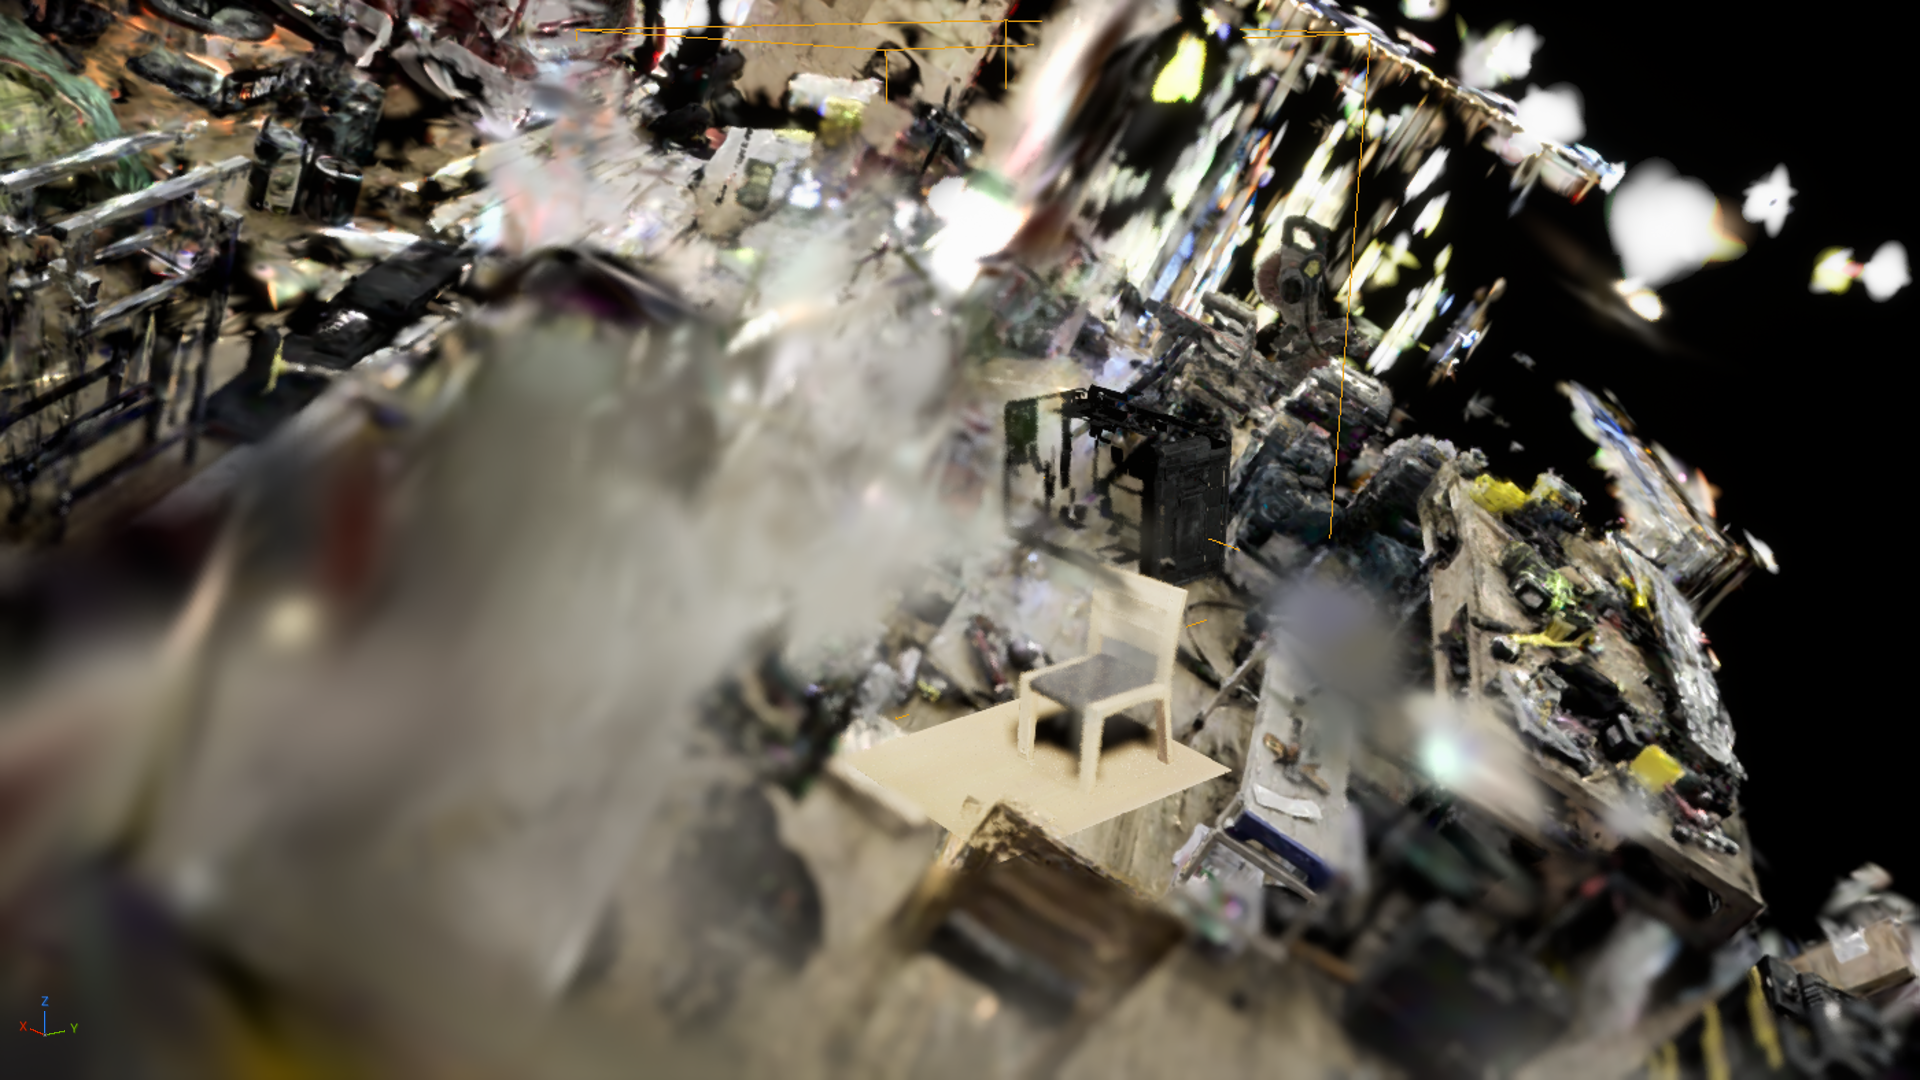
\includegraphics[width=\textwidth]{figures/scene_integrated.png}
  \caption{%
    \textbf{Integrated UE\,5.8 scene — room splat with placed TRELLIS.2 object FBXs.}
    The assembled deliverable: NanoGS splat room (hero representation) with
    chair, vacuum, and toolbox FBXs (TRELLIS.2 \texttt{hull\_e2e},
    prescaled via \texttt{blender\_prescale\_objects}) placed by
    \texttt{ue\_place\_prescaled}.
    Objects are Nanite game assets with baked PBR textures; the room splat
    renders real Gaussians.
    This image is the \emph{docs} canonical integrated-scene reference.
  }
  \label{fig:scene_integrated}
\end{figure}

% ──────────────────────────────────────────────────────────────────────────────
% 6. TRELLIS.2 object turnaround sheet (chair)
% ──────────────────────────────────────────────────────────────────────────────
\begin{figure}[htbp]
  \centering
  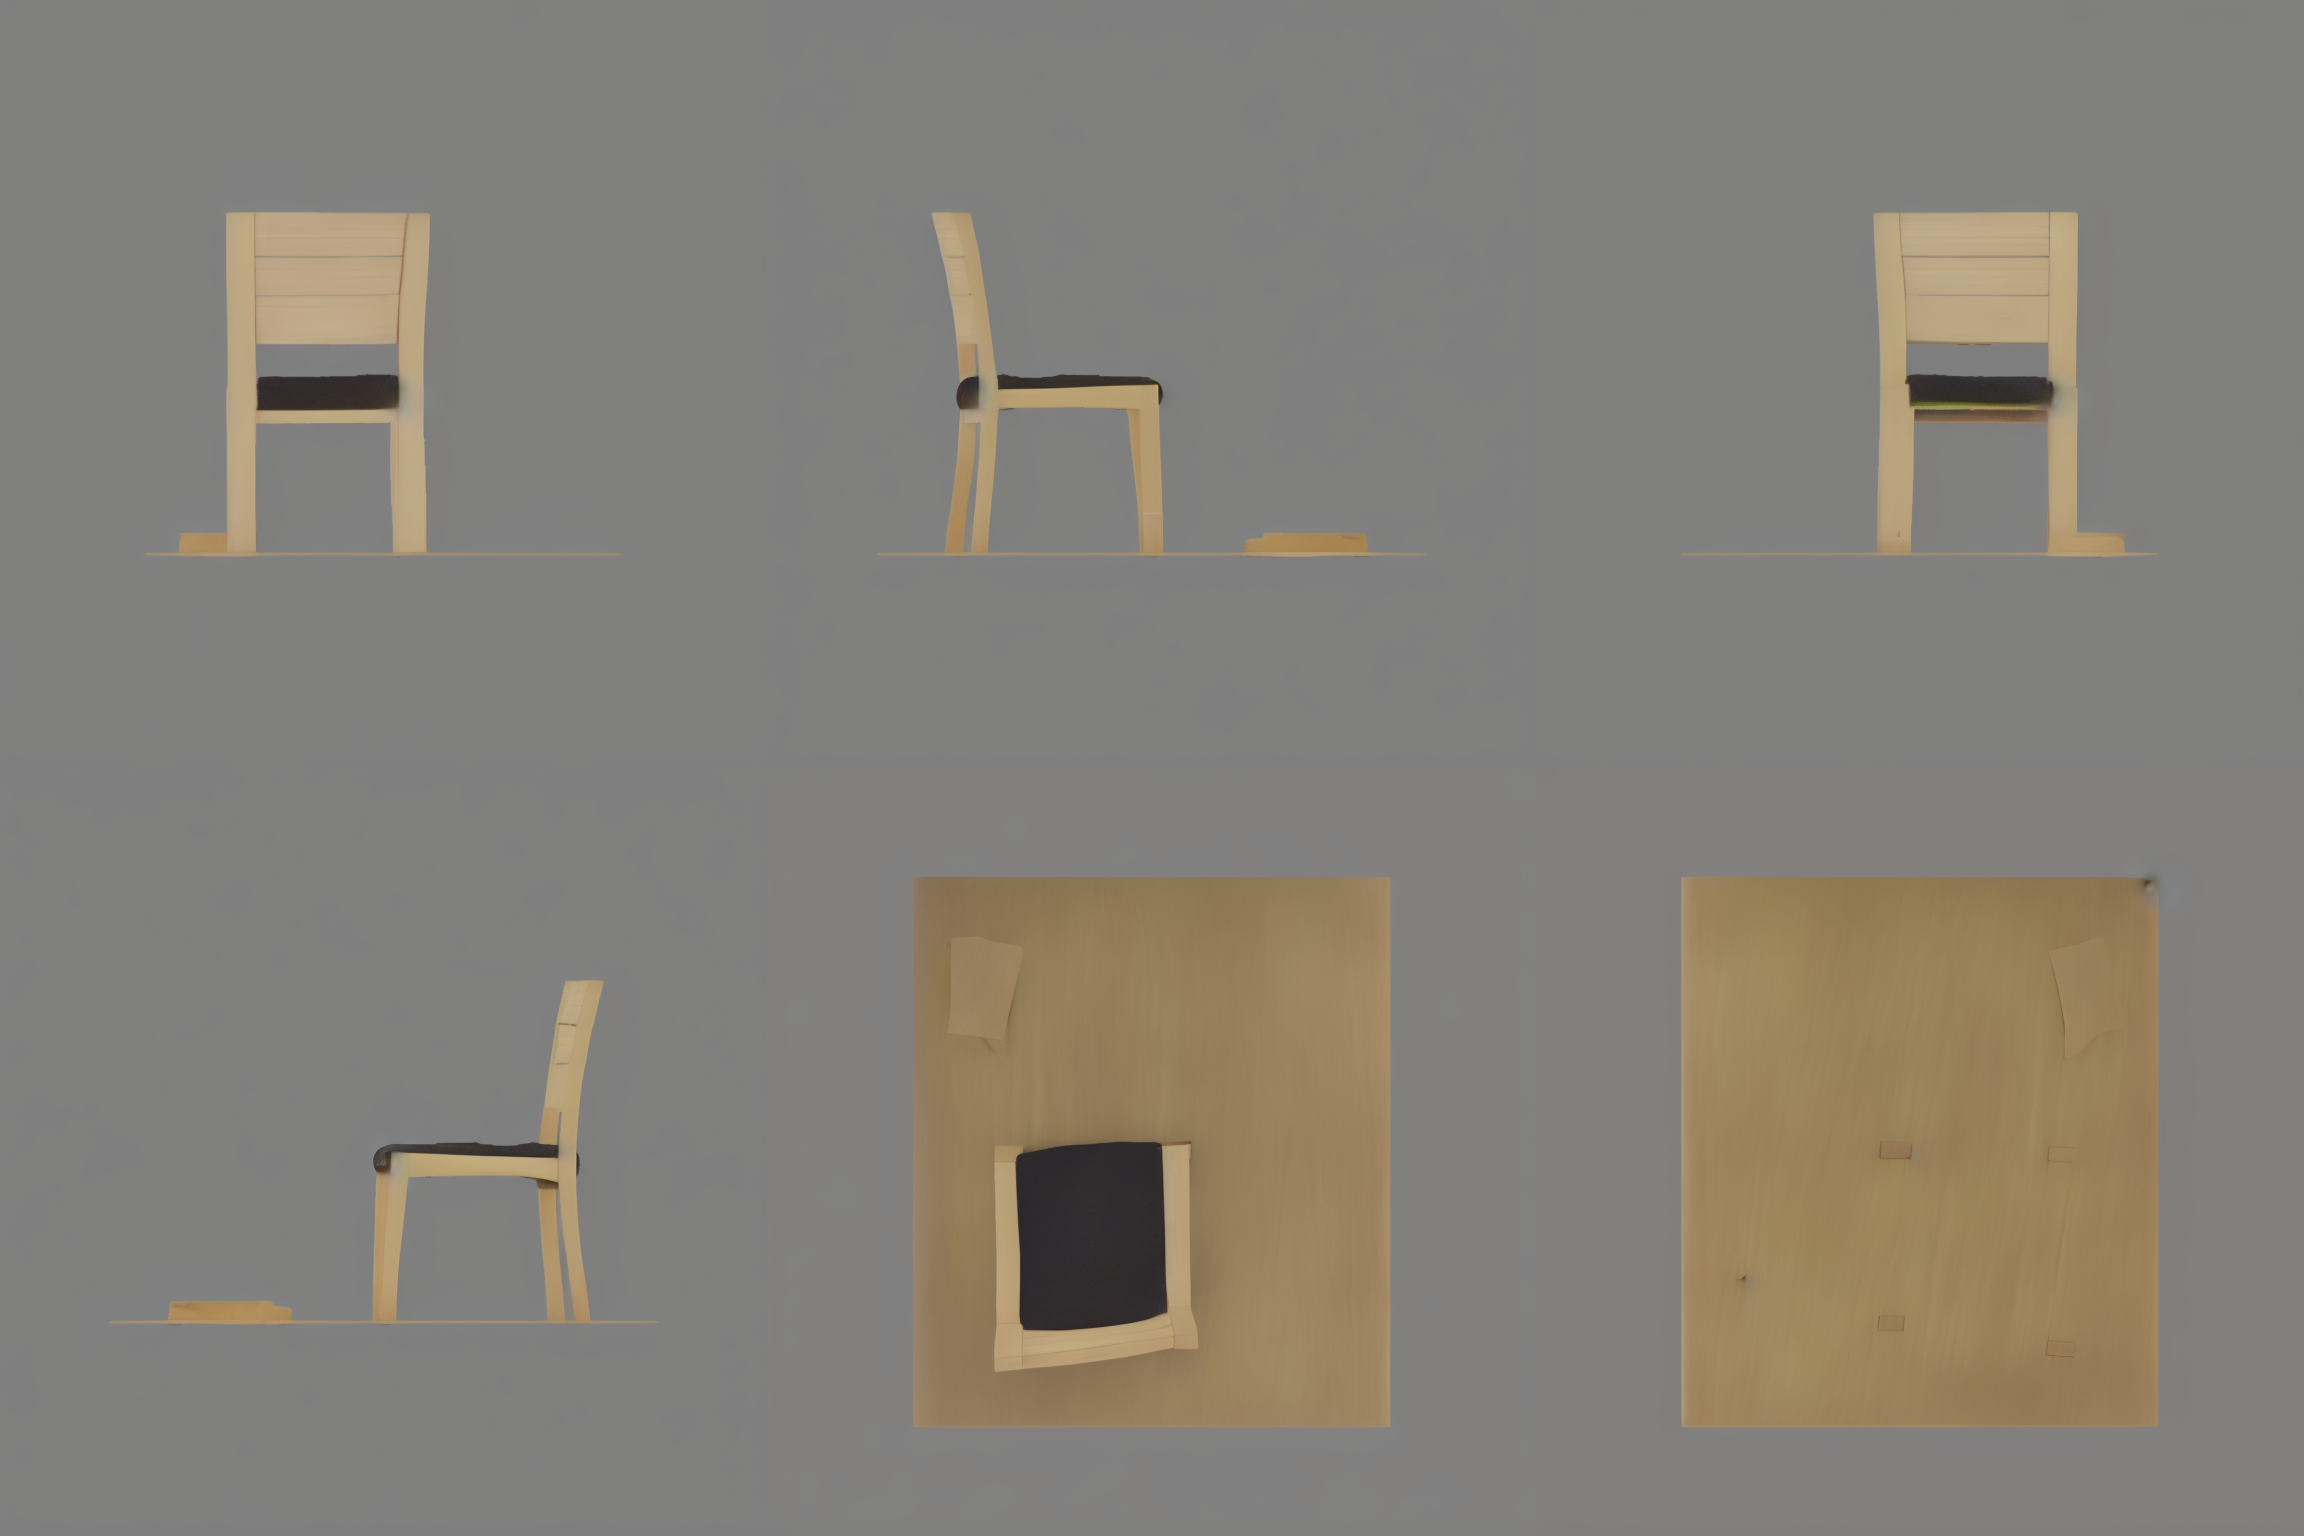
\includegraphics[width=\textwidth]{figures/chair_turnaround_sheet.png}
  \caption{%
    \textbf{TRELLIS.2 object reconstruction — chair turnaround sheet.}
    Multi-view orbit render of the textured GLB mesh produced by the
    \texttt{hull\_e2e} workflow: per-object SAM3 PLY crop $\to$ FLUX.2-dev
    view-inpainting $\to$ TRELLIS.2-4B mesh $\to$ PBR-baked GLB $\to$ FBX
    (Nanite game asset).
    The chair is rated \emph{good}; vacuum and toolbox likewise passed
    the object reconstruction gate (4/8 objects in this batch).
    Resolution: 2304$\times$1536.
  }
  \label{fig:objects}
\end{figure}

% ──────────────────────────────────────────────────────────────────────────────
% 7. CoMe-TSDF mesh in UE (baseline mesh deliverable)
% ──────────────────────────────────────────────────────────────────────────────
\begin{figure}[htbp]
  \centering
  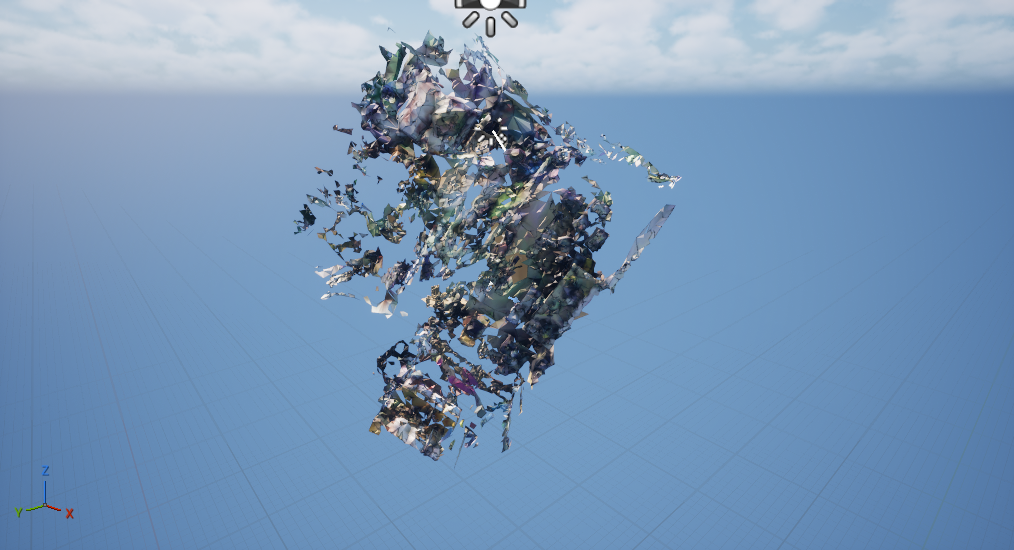
\includegraphics[width=\textwidth]{figures/ue_come_final.png}
  \caption{%
    \textbf{CoMe-TSDF room mesh game asset in UE\,5.8 (baseline mesh deliverable).}
    The scene-mesh branch: CoMe legacy \texttt{ScalableTSDFVolume} extraction,
    \texttt{mesh\_cleaner} (smooth=0, edge-length + connected-component cleanup),
    xatlas bake (\texttt{bake\_from\_vertex\_colors}), \texttt{blender\_obj\_to\_fbx},
    imported as a Nanite mesh.
    Characteristic TSDF blockiness on flat walls is visible; this image
    motivates the re-spine to NanoGS as the default room representation for
    blur-limited captures.
    Resolution: 1014$\times$550.
  }
  \label{fig:ue_come}
\end{figure}

% ──────────────────────────────────────────────────────────────────────────────
% 8. NanoGS splat render (1920×1080 B-view)
% ──────────────────────────────────────────────────────────────────────────────
\begin{figure}[htbp]
  \centering
  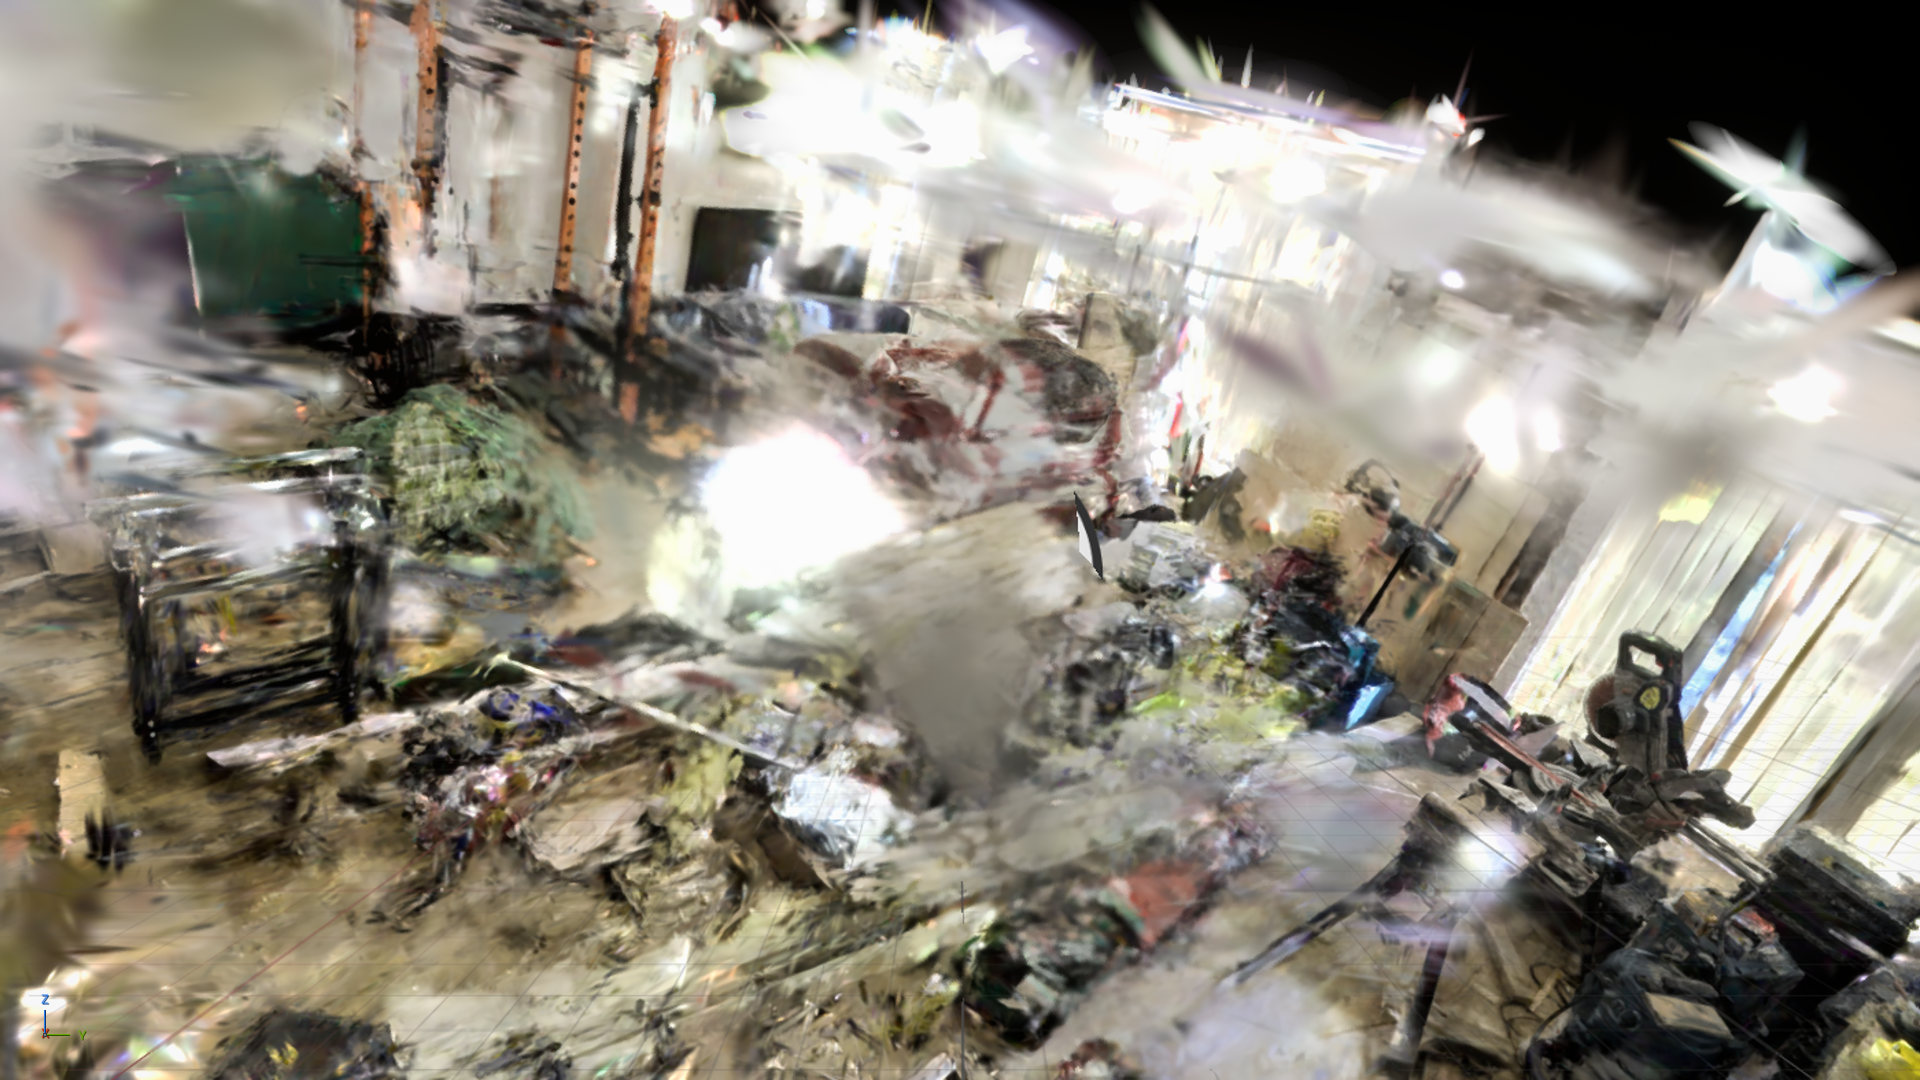
\includegraphics[width=\textwidth]{figures/ue_nanogs_room_B.png}
  \caption{%
    \textbf{NanoGS real-Gaussian splat in UE\,5.8 — interior view (B).}
    Second viewpoint of the NanoGS splat room, demonstrating depth and
    parallax of real Gaussian rendering at 1920$\times$1080.
    Comparison with Figure~\ref{fig:ue_come} illustrates the quality
    improvement of splat-hero over TSDF mesh for a motion-blur-limited
    capture: the splat faithfully preserves captured radiance;
    the mesh introduces geometric artefacts irrelevant to the capture.
  }
  \label{fig:ue_nanogs}
\end{figure}

% ──────────────────────────────────────────────────────────────────────────────
% 9. Hero perspective render (room + placed objects)
% ──────────────────────────────────────────────────────────────────────────────
\begin{figure}[htbp]
  \centering
  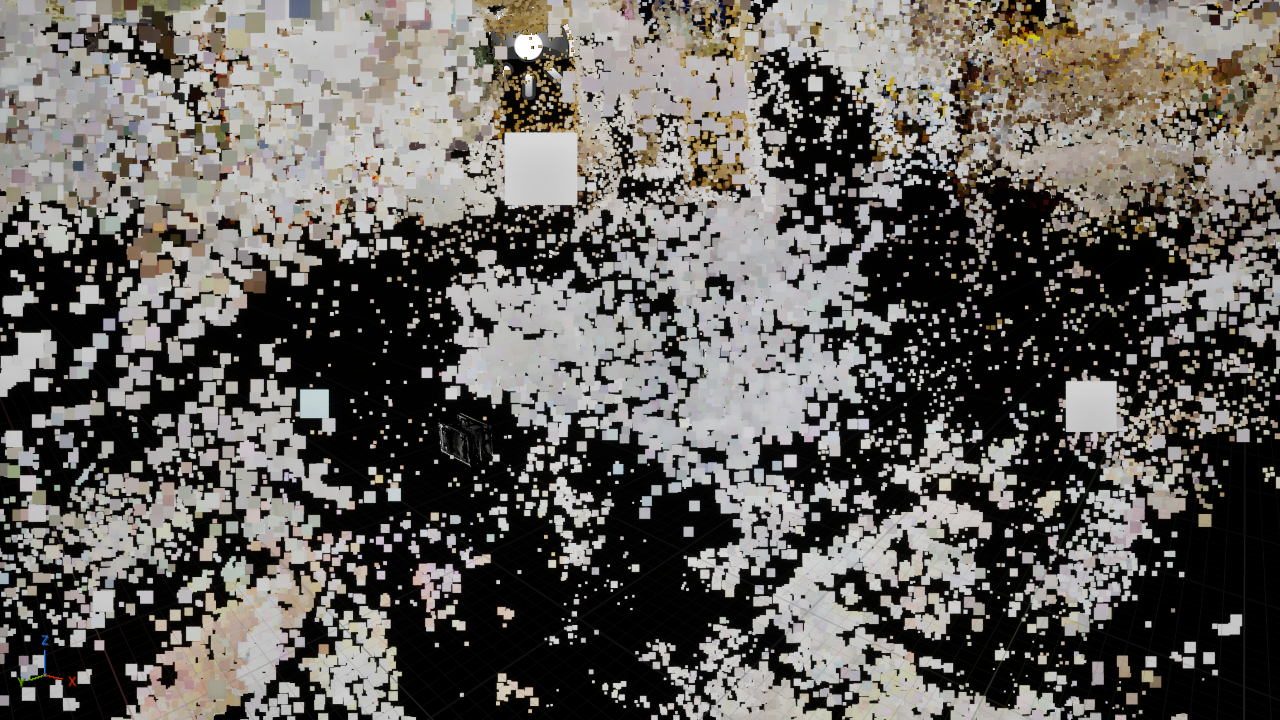
\includegraphics[width=\textwidth]{figures/ue_final_hero.png}
  \caption{%
    \textbf{Hero perspective render — dreamlab room with placed object FBXs.}
    A cinematic view of the assembled UE\,5.8 scene from the validated
    end-to-end run (2026-06-22): TSDF-mesh room (CoMe, pre-NanoGS re-spine)
    with TRELLIS.2 object FBXs placed by \texttt{ue\_place\_prescaled}.
    Resolution: 1280$\times$720.
    Serves as the primary before/after reference for evaluating the
    NanoGS re-spine (Figure~\ref{fig:nanogs_room}).
  }
  \label{fig:ue_hero}
\end{figure}

% ──────────────────────────────────────────────────────────────────────────────
% 10. Overhead dollhouse view
% ──────────────────────────────────────────────────────────────────────────────
\begin{figure}[htbp]
  \centering
  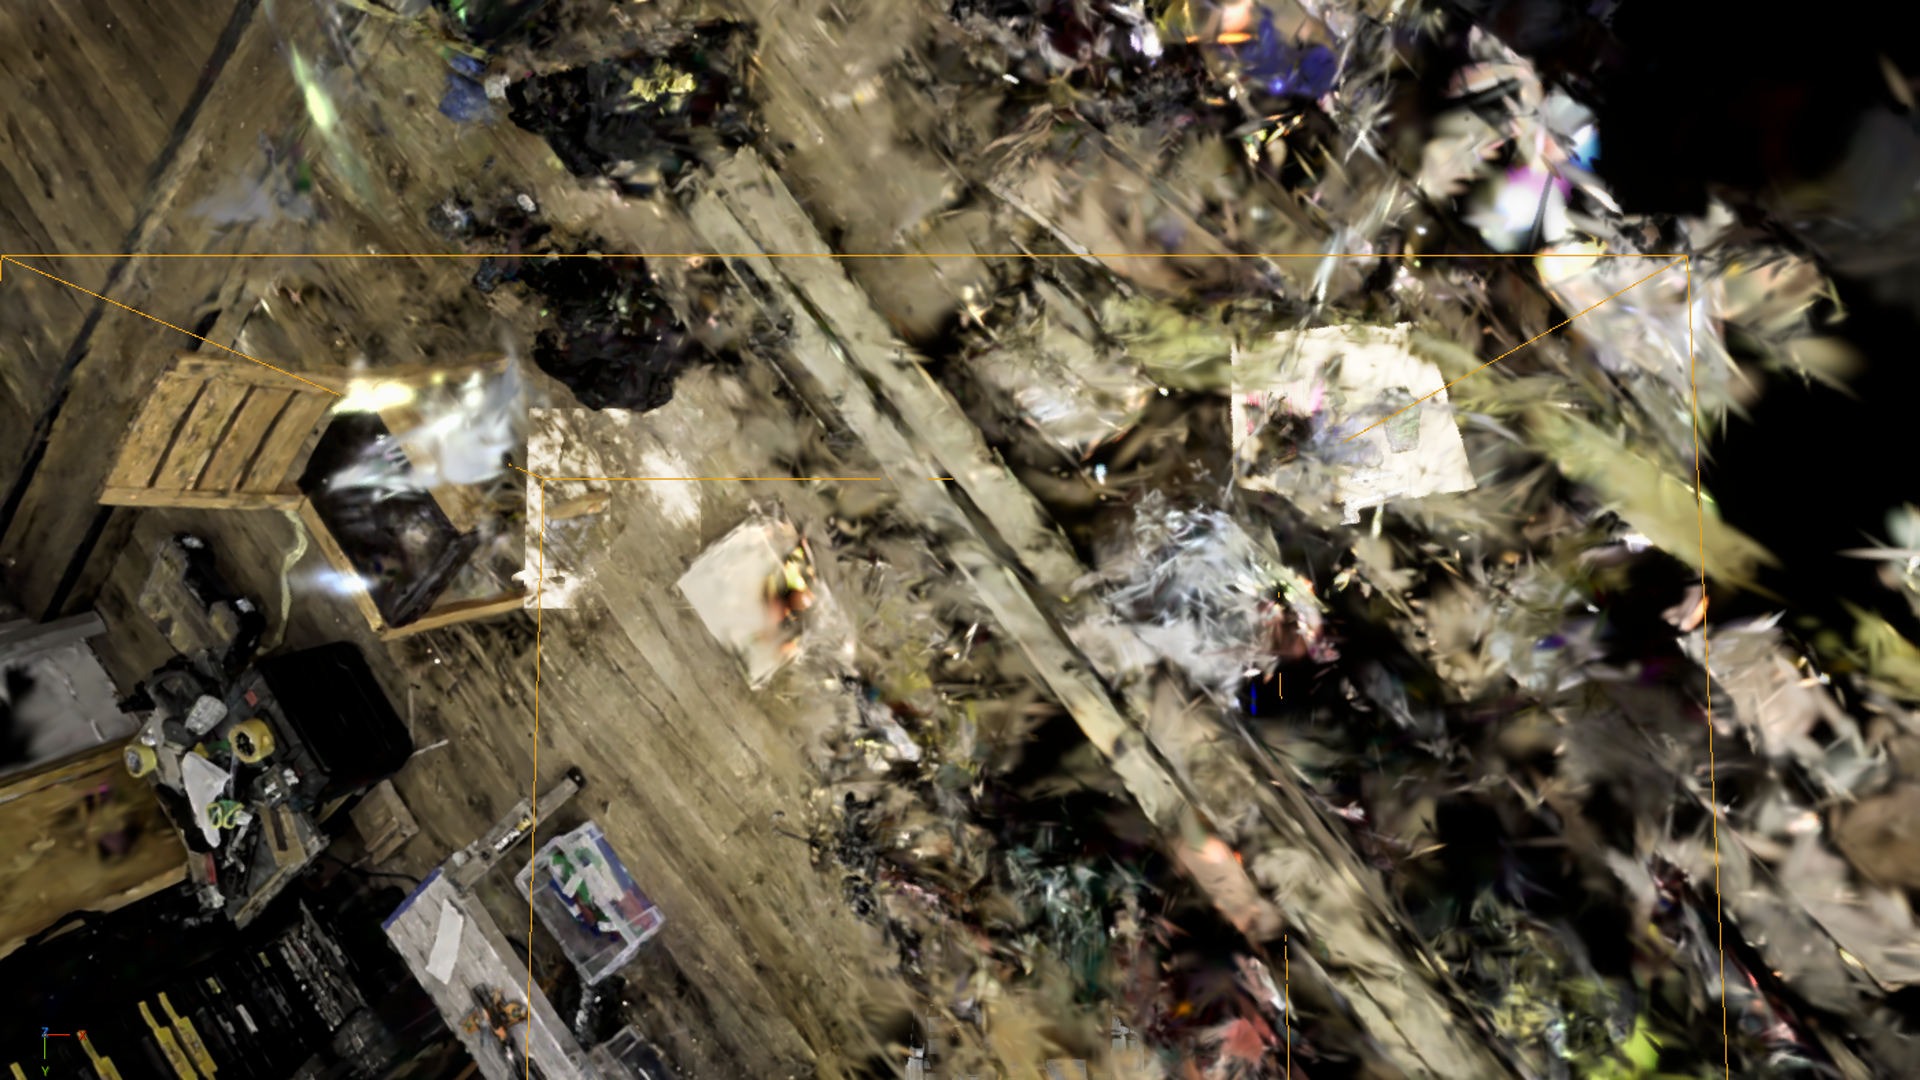
\includegraphics[width=\textwidth]{figures/ue_integrated_dollhouse.png}
  \caption{%
    \textbf{Overhead dollhouse view — integrated UE\,5.8 scene layout.}
    Top-down perspective revealing object placement, room geometry, and
    spatial relationships of the dreamlab scene.
    The dollhouse view is the standard QA checkpoint for scale fidelity
    and object-in-room alignment after \texttt{ue\_place\_prescaled}
    prescaling.
    Resolution: 1920$\times$1080.
  }
  \label{fig:ue_dollhouse}
\end{figure}


% ====================================================================
\appendix
% appendix_playbook.tex — Vitrine Operator Playbook
% Practical user-guide appendix for the v5 report.
% Wire into main with:
%   \appendix
%   % appendix_playbook.tex — Vitrine Operator Playbook
% Practical user-guide appendix for the v5 report.
% Wire into main with:
%   \appendix
%   % appendix_playbook.tex — Vitrine Operator Playbook
% Practical user-guide appendix for the v5 report.
% Wire into main with:
%   \appendix
%   \input{v5/appendix_playbook}
%
% Dr John O'Hare, DreamLab AI Consulting Ltd — June 2026

% =====================================================================
\chapter{Operator Playbook: Running Vitrine End-to-End}
\label{app:playbook}
% =====================================================================

This appendix is a practical guide for a new operator.  It assumes the Docker
stack is accessible but does not assume familiarity with the internals; the
steps call the pipeline through its published Python and REST interfaces.
Read the capture section (\S\ref{sec:pb-capture}) before anything else:
\emph{capture quality is the single largest determinant of output quality},
and no downstream step can compensate for footage that was never sharp.

% ─────────────────────────────────────────────────────────────────────
\section{Capture Methodology: The Dominant Quality Lever}
\label{sec:pb-capture}
% ─────────────────────────────────────────────────────────────────────

\begin{keyfinding}
Motion blur is the dominant failure mode in practice.  Empirical measurement
on the \emph{dreamlab} dataset found zero under-observed area (median
$\approx$\,90 cameras per surface point) yet a holey, noisy reconstruction.
The problem was dense-but-motion-blurred footage, not insufficient coverage.
Blur cannot be recovered in post: selection can raise the sharpness floor, but
it cannot create detail the sensor never recorded.
\end{keyfinding}

\subsection{Camera settings}
\label{sec:pb-camera-settings}

Lock all automatic adjustments before pressing record.  Any automatic change
between frames is interpreted by COLMAP as a change in scene appearance and
degrades feature matching.

\begin{center}
\begin{tabular}{@{}L{3.2cm}L{4.8cm}L{5.8cm}@{}}
\toprule
\textbf{Setting} & \textbf{Recommendation} & \textbf{Why} \\
\midrule
Resolution     & 4K (3840$\times$2160)           & More features per frame; 8K adds storage cost without proportional gain as training downsamples anyway \\
Frame rate     & \textbf{60\,fps}                 & Caps exposure to $\leq$\,1/60\,s vs.\ 1/30\,s at 30\,fps, halving motion blur; also doubles the candidate frames for sharpness selection \\
Focus          & Manual, mid-distance (3--5\,m)  & Autofocus hunting softens frames and breaks feature matching \\
Exposure       & Manual, locked                  & Auto-exposure causes frame-to-frame brightness ramps that COLMAP interprets as surface-appearance changes \\
White balance  & Manual preset                   & Auto white balance shifts colour temperature between frames \\
Shutter speed  & $\geq$\,1/500\,s (lock in pro app) & Short exposure is the primary anti-blur lever; bright, even light lets you achieve this without under-exposure \\
Lens           & 24--50\,mm equivalent (1$\times$ main camera on phones) & Minimal distortion; ultra-wide ($<$16\,mm) fails in periphery; telephoto reduces parallax \\
\bottomrule
\end{tabular}
\end{center}

\medskip
\noindent\textbf{Phone-specific note.}  Flagship phones (iPhone 15 Pro,
Pixel 9 Pro, Samsung S24 Ultra) produce usable video \emph{only} if you use
the main 1$\times$ camera, lock exposure, focus, and white balance via a pro
app (e.g.\ mcpro24fps, FiLMiC Pro), and shoot in good light.  The Pixel 9 Pro
experiment found \textbf{4K/60\,fps} to be the best video mode: 60\,fps caps
exposure and doubles candidate frames.  \textbf{8K/30\,fps is worse}: the
longer exposure from 30\,fps produces blurrier frames; extra pixels on a
blurred frame are wasted.  If the camera supports RAW photo bursts, those are
even better --- very short exposure, no inter-frame compression.

\subsection{Movement and stabilisation}
\label{sec:pb-movement}

\begin{itemize}
  \item \textbf{Maximum walking speed: 0.5\,m/s.}  Counting ``one-Mississippi''
        per step is a practical governor.  When in doubt, slow down further.
  \item \textbf{Use a gimbal} (DJI RS, Zhiyun) or a tripod dolly.  These
        eliminate micro-shake and rolling-shutter artefacts.  Two-handed
        handheld capture is marginal in bright light; single-hand phone capture
        introduces motion blur on most frames and should be avoided.
  \item \textbf{Insert micro-pauses} at key viewpoints.  The sharpness
        sampler harvests the sharp still frames from these pauses.  Even a
        fraction of a second of steadiness at a corner or interesting object is
        worth more than continuous motion.
  \item \textbf{Move laterally, not just forward.}  The pipeline needs
        triangulation, and triangulation needs physical baseline between
        viewpoints.  Sidestep, arc, and weave rather than walking straight ahead.
  \item \textbf{Every point in the scene should be visible from at least five
        viewpoints.}  Revisit areas from different angles rather than passing
        through once.
\end{itemize}

\subsection{Capture patterns}
\label{sec:pb-patterns}

\paragraph{Room scan (60--120\,s per room).}
Walk the full perimeter at three height bands — low ($\approx$\,1\,m, waist),
eye level ($\approx$\,1.6\,m), and high (arms raised, $\approx$\,2.2\,m) —
then walk the two diagonals to fill the interior.  This gives three elevation
bands of every wall plus cross-coverage of floor and ceiling.  Multiple
independent sweeps of the same room at different heights combine into a denser
reconstruction than any single sweep: an observed three-sweep capture produced
$\approx$146\,k COLMAP points at $\approx$95\,\% registration versus $\approx$90\,k
at $\approx$90\,\% for a single perimeter pass.

\paragraph{Object orbit (30--60\,s per object).}
The best room sweep is rarely the best for any individual object.  Objects you
want as individual hulls need a \emph{dedicated} close orbit in addition to
the room sweeps:
\begin{enumerate}[nosep]
  \item Orbit at eye level ($\approx$1.5\,m distance): full 360°, 20\,s.
  \item Orbit at knee height, camera angled upward: full 360°, 20\,s.
  \item Orbit above head, camera angled downward: full 360°, 20\,s.
\end{enumerate}

\paragraph{Detail pass (10--15\,s per feature).}
After room and object passes, sweep 30--50\,cm from important surfaces (carved
detail, lettering, fine texture).  These close-up frames lift the resolution
ceiling for that region.

\subsection{Scene preparation}
\label{sec:pb-scene-prep}

\begin{itemize}
  \item \textbf{Remove all moving elements.}  People, animals, ceiling fans,
        screens playing video, swaying plants — any inter-frame motion creates
        smeared ghost geometry.  Pause recording if someone walks through the
        scene.  Even a person standing still shifts weight and breathes.
  \item \textbf{Turn screens off.}  A powered-off TV is far less glossy than a
        running one.  A running TV is the worst-case object: a large,
        view-dependent reflector whose reflections defeat both SfM (inconsistent
        features) and 3DGS (spherical-harmonics overfit the moving reflection
        into floaters).  The 2026-06-21 Drive dataset was abandoned for exactly
        this reason combined with low MUSIQ scores.
  \item \textbf{Cover mirrors and polished surfaces.}  Matte fabric or dulling
        spray prevents ghost geometry behind reflective surfaces.
  \item \textbf{Ensure even, diffuse lighting.}  Overcast sky is ideal outdoors.
        Indoors, use large soft panels or bounce lights off the ceiling.  Before
        recording, rotate 360° in the scene centre watching the exposure meter:
        if it swings more than 1.5 stops, add fill light or flag bright sources.
  \item \textbf{Add temporary texture to featureless surfaces.}  White walls and
        plain ceilings give COLMAP nothing to match.  Place books, plants, or
        patterned cloth against blank walls during capture; remove them later if
        needed.
\end{itemize}

\subsection{Do / do not summary}
\label{sec:pb-donot}

\begin{center}
\begin{tabular}{@{}L{5.8cm}L{7.2cm}@{}}
\toprule
\textbf{Do} & \textbf{Do not} \\
\midrule
4K/60\,fps, manual exposure, focus, WB & Use auto-exposure or auto white balance \\
Gimbal or two-handed stabilisation & Pan fast ($>$15°/s) or shoot single-handed \\
$\leq$\,0.5\,m/s, micro-pauses at key points & Walk at normal pace \\
Three height bands + diagonals & Walk only one straight path through the space \\
Dedicated 360° object orbits & Assume the room sweep covers individual objects \\
Transfer the original camera file over USB & Upload to a cloud service that transcodes \\
Even, diffuse lighting & Mix tungsten and daylight; allow hard shadows \\
Turn screens and fans off & Capture with any motion in the scene \\
$\geq$1/500\,s shutter (lock in pro app) & Rely on in-camera optical stabilisation alone for blur \\
4K/60\,fps on phones & Use 8K/30\,fps (blurrier despite higher pixel count) \\
\bottomrule
\end{tabular}
\end{center}

\subsection{Why blur is unrecoverable}
\label{sec:pb-blur-unrecoverable}

Motion blur is a measurement artefact: a blurred pixel is the average of many
spatial samples acquired over the exposure window, and the individual samples
are gone.  Per-frame generative deblurring (NAFNet, Restormer) hallucinates
texture rather than recovering it, and the hallucinated texture is spatially
inconsistent across frames, which breaks multi-view SfM.  The only
reconstruction methods that legitimately model blur --- joint exposure-trajectory
optimisation approaches such as \textsc{3dgs-deblur} --- show gains of
approximately 1--2\,dB PSNR on \emph{moderate} blur but hit the same
SfM-quality ceiling as the source footage.  \textbf{Blur is unrecoverable in
post; the real lever is short-shutter capture.}

The Vitrine frame-QA gate applies a MUSIQ no-reference IQA score plus a full-resolution
variance-of-Laplacian sharpness score to every extracted frame.  A video that cannot
supply \code{min\_good\_frames} above the KEEP threshold is marked
\code{too\_low\_quality} and the operator is asked to recapture.  The dreamlab
dataset scored a median MUSIQ of $\approx$\,31 (usable but blur-limited); the
abandoned Drive dataset scored $\approx$\,19 (unusable).  The gate is a diagnostic,
not a repair: it tells you when recapture is necessary.

% ─────────────────────────────────────────────────────────────────────
\section{Running the Pipeline}
\label{sec:pb-run}
% ─────────────────────────────────────────────────────────────────────

\subsection{Bringing up the stack}
\label{sec:pb-stack}

All pipeline work runs inside the \code{gaussian-toolkit} container.  From the
repository root on the host:

\begin{lstlisting}[language=bash,caption={Bring up the consolidated stack}]
# Clone with the vendored LichtFeld tool included
git clone --recurse-submodules <repo-url>
cd Vitrine

# Start the pipeline containers (GPU required)
docker compose -f docker-compose.consolidated.yml up -d

# Verify the stack is healthy
curl http://gaussian-toolkit:7860/health     # web UI
curl http://gaussian-toolkit:45677/mcp       # LichtFeld MCP
curl http://vitrine-comfyui:8188/system_stats  # ComfyUI (TRELLIS.2 / FLUX.2)
\end{lstlisting}

\noindent The Unreal Engine 5.8 overlay is optional and started separately:

\begin{lstlisting}[language=bash,caption={Bring up the Unreal overlay (optional)}]
docker compose \
  -f docker-compose.consolidated.yml \
  -f unreal/docker-compose.unreal.yml \
  up -d unreal unreal-mcp-bridge
\end{lstlisting}

\noindent Run the SOTA preflight check to verify model weights and VRAM before
processing any footage:

\begin{lstlisting}[language=bash,caption={SOTA preflight}]
python -m pipeline.sota_registry check
\end{lstlisting}

\noindent If any weight or pin is stale the preflight reports it; resolve before
continuing.  Model weights live in \code{data/comfyui/models/} ($\approx$\,216\,GB,
bind-mounted read-only); do not re-download them.

\subsection{Ingest and frame QA}
\label{sec:pb-ingest}

Place source video files in \code{data/raw/} and submit the job via the web UI
(\texttt{http://localhost:7860}) or directly:

\begin{lstlisting}[language=bash,caption={Step 1 -- ingest and frame extraction}]
python3 -c "
from pipeline.stages import PipelineStages
p = PipelineStages('/data/output/JOB_ID')
result = p.ingest('/data/raw/scene.mp4', fps=4.0)
print(result)
"
\end{lstlisting}

\noindent Ingest extracts frames at 4\,fps to oversample, then the frame-QA
stage selects the sharpest subset.  The QA pipeline applies two complementary
metrics:

\begin{enumerate}
  \item \textbf{MUSIQ no-reference IQA} (\code{pyiqa}, GPU).  A
        perceptual score on the KonIQ-10k scale ($\approx$0--100; good
        photography scores 50--75; severely blurred or noisy footage scores
        below $\approx$25).  Videos unable to supply enough frames above the
        KEEP threshold are marked \code{too\_low\_quality} and skipped.
  \item \textbf{Full-resolution variance-of-Laplacian.}  Sharpness is measured
        at full 4K resolution, not at a downscaled proxy --- downscaling blurs
        away the motion-blur signal (960p blurdetect showed only a
        $\approx$1.6$\times$ range on dreamlab frames; full-4K Laplacian showed a
        $\approx$105$\times$ range).  The \emph{sharpest frame per overlapping
        FIFO window} is kept, which raises the sharpness floor by 20--38\,\% at
        the bottom quartile --- the frames that most poison COLMAP matches.
\end{enumerate}

\noindent Inspect the selected frame count before proceeding:

\begin{lstlisting}[language=bash,caption={Step 3 -- select best frames}]
python3 -c "
from pipeline.stages import PipelineStages
p = PipelineStages('/data/output/JOB_ID')
result = p.select_frames('/data/output/JOB_ID/frames/', target=80)
print(result)
"
# Target: 60-80 frames. If < 40 are above threshold, consider recapture.
\end{lstlisting}

\subsection{Structure-from-Motion and 3DGS training}
\label{sec:pb-sfm-train}

\begin{lstlisting}[language=bash,caption={Step 4 -- COLMAP SfM (sequential matcher for video)}]
python3 -c "
from pipeline.stages import PipelineStages
p = PipelineStages('/data/output/JOB_ID')
result = p.reconstruct('/data/output/JOB_ID/frames_selected/',
                       matcher='sequential')
print(result)
"
# Quality gate: >= 70 % of frames must register.
# If < 50 % register, re-run with matcher='exhaustive'.
\end{lstlisting}

\begin{lstlisting}[language=bash,caption={Step 5 -- 3DGS training (30\,000 iterations)}]
python3 -c "
from pipeline.stages import PipelineStages
p = PipelineStages('/data/output/JOB_ID')
result = p.train('/data/output/JOB_ID/colmap/undistorted/',
                 iterations=30000)
print(result)
"
# Quality gate: PLY file should be > 10 MB; loss < 0.02.
\end{lstlisting}

\noindent The output splat is \code{output/JOB\_ID/model/splat\_30000.ply}.  This
file is the primary LichtFeld-native deliverable that feeds both the Gaussian
splat room path and the object segmentation branch.

\subsection{The stage sequence}
\label{sec:pb-sequence}

The full pipeline in order:

\begin{center}
\begin{tabular}{@{}lL{4.5cm}L{6cm}@{}}
\toprule
\textbf{Stage} & \textbf{What runs} & \textbf{Quality check} \\
\midrule
1 & Ingest: frame extraction at 4\,fps & \code{frames/} directory populated \\
2 & Remove people (if present) & Inspect sample frames \\
3 & Frame-QA selection & 60--80 KEEP-grade frames \\
4 & COLMAP SfM (sequential matcher) & $\geq$\,70\,\% registration \\
5 & 3DGS training (30\,k iterations) & PLY $>$10\,MB, loss $<$0.02 \\
6 & SAM3 concept segmentation & $\geq$\,2 objects identified \\
7 & Per-object PLY extraction + orbit renders & $\geq$5\,k vertices per object \\
7c & TRELLIS.2 hull\_e2e (textured GLB) & Textured GLB produced per object \\
8 & Room mesh extraction (TSDF or 2DGS) & $\geq$\,30\,k vertices, clean topology \\
8b & Mesh cleanup (\code{mesh\_cleaner smooth=0}) & No stray bridging triangles \\
8c & Texture bake (xatlas UV + vertex colours) & Texture atlas per mesh \\
9 & FBX export (\code{blender\_obj\_to\_fbx}) & FBX files produced \\
9b & UE 5.8 import (Nanite game assets) & Assets visible in Content Browser \\
10 & Validate + job complete & Full scene: room + objects \\
\bottomrule
\end{tabular}
\end{center}

\noindent \textbf{Do not stop after training.}  The pipeline is only complete
when it reaches the textured UE scene; stopping at the splat leaves the
deliverable unfinished.

% ─────────────────────────────────────────────────────────────────────
\section{Per-Capture Recipe Selection}
\label{sec:pb-recipe}
% ─────────────────────────────────────────────────────────────────────

Vitrine is not a fixed pipeline.  Each capture is \emph{diagnosed} first; the
router selects the configuration that best fits the capture's bottleneck.  The
four diagnostic axes are:

\begin{description}
  \item[Sharpness] Measured by MUSIQ + full-resolution Laplacian.  Is the
    footage blur-limited?
  \item[Coverage] Measured by a per-surface-point viewpoint count.  Are there
    under-observed regions (holes) or is coverage uniformly dense?
  \item[Hardware] RGB camera only, depth sensor (iPhone LiDAR), or event camera?
  \item[Deliverable] Fidelity-first splat room, polygonal mesh room, or both?
\end{description}

\noindent Table~\ref{tab:pb-recipes} maps common capture profiles to their
recommended configurations.

\begin{table}[ht]
\centering
\caption{Capture profile to recipe selector.  Objects are always reconstructed
via TRELLIS.2 \code{hull\_e2e} regardless of room profile.}
\label{tab:pb-recipes}
\begin{tabular}{@{}L{3.4cm}L{2.4cm}L{2.4cm}L{2.2cm}L{3.0cm}@{}}
\toprule
\textbf{Capture profile} & \textbf{Room rep} & \textbf{Enhancer} & \textbf{Mesh backend} & \textbf{Note} \\
\midrule
\textbf{Blurry $\cdot$ dense $\cdot$ RGB}
  (e.g.\ dreamlab)
  & Splat hero + mesh asset (dual)
  & \emph{None} (ArtiFixer won't help)
  & 2DGS / PGSR
  & Recapture is the real ceiling \\
\addlinespace
\textbf{Sharp $\cdot$ holey $\cdot$ RGB}
  & Splat (primary)
  & \textbf{ArtiFixer} (fills floaters/holes)
  & 2DGS / PGSR if mesh required
  & ArtiFixer's sweet spot \\
\addlinespace
\textbf{Sharp $\cdot$ dense $\cdot$ RGB}
  & Splat (primary)
  & None
  & 2DGS if mesh needed
  & Best case; least pain \\
\addlinespace
\textbf{iPhone LiDAR depth}
  & Mesh (primary)
  & Optional
  & \textbf{AGS-Mesh} (sensor depth)
  & Depth sensor unlocks clean walls \\
\addlinespace
\textbf{Event camera $\cdot$ blurry}
  & Splat
  & ---
  & ---
  & EBAD-Gaussian deblurs at source \\
\bottomrule
\end{tabular}
\end{table}

\subsection{Splat vs.\ mesh for the room}
\label{sec:pb-splat-vs-mesh}

\textbf{Default --- room as splat (NanoGS in UE 5.8).}  For an indoor room the
recommended default is to represent the room as a real Gaussian splat rendered
by the NanoGS UE 5.8 plugin, with object FBXs from TRELLIS.2 embedded
alongside it.  This is simultaneously the highest-fidelity path and the one
that leans most directly on the vendored LichtFeld trainer: the native
\code{splat\_30000.ply} is cleaned with SuperSplat, imported into UE 5.8, and
rendered as real Gaussians.  The mandated polygonal mesh is satisfied by the
TRELLIS.2 object FBXs.

\textbf{When to use a polygonal room mesh.}  If the brief requires a fully
polygonal game-asset scene (Nanite room mesh, not a splat), use \textbf{2DGS}
(quick win, same Open3D-TSDF backend as the current fallback, but 2D-surfel
depth is much cleaner than ellipsoid depth on flat walls) or \textbf{PGSR}
(planar Gaussians, explicitly handles textureless walls, strongest for indoor
rooms).  The legacy CoMe/Open3D-TSDF combination is retained as a fallback
but produces visibly blockier results and should not be the default.

\textbf{When ArtiFixer helps.}  ArtiFixer is a 3DGS refiner targeting
floaters, holes, and under-observed regions: it applies an opacity-mix
enhancement that fills in areas seen from too few viewpoints.  It runs on a
single 48\,GB RTX 6000 Ada (peak $\approx$\,45.5\,GB) and is the correct tool
for \emph{sharp but coverage-limited} captures.  It does \emph{not} deblur.
Applying ArtiFixer to a blur-limited capture wastes GPU time without improving
results.

\textbf{NanoGS floaters.}  The NanoGS plugin renders the splat faithfully,
including any floater Gaussians in the source PLY.  Pre-clean the PLY with
SuperSplat (floater removal by opacity and scale thresholds) before import.
If floaters persist after SuperSplat, check whether coverage was the issue
(ArtiFixer) or whether the source footage was simply blurry (recapture).

\subsection{Object reconstruction}
\label{sec:pb-objects}

Objects follow the same path regardless of room profile:

\begin{enumerate}
  \item \textbf{SAM3 concept segmentation} identifies freestanding objects in
        the splat and extracts per-object Gaussian PLY subsets.
  \item \textbf{Orbit render}: four synthetic camera views around the object
        centroid are rendered from the Gaussian subset.
  \item \textbf{TRELLIS.2 \code{hull\_e2e}}: the orbit renders are submitted to
        TRELLIS.2 (via ComfyUI at \code{http://vitrine-comfyui:8188}) which runs
        FLUX.2 turnaround generation followed by TRELLIS.2 3D reconstruction,
        producing a textured GLB with PBR materials.
  \item \textbf{Prescale}: Blender prescales the GLB to physical units to match
        the COLMAP coordinate frame.
  \item \textbf{FBX export}: the prescaled mesh is exported as FBX for UE 5.8
        game-asset import (Nanite-ready).
\end{enumerate}

\noindent TRELLIS.2 is the validated primary path; Hunyuan3D-2.1 (also staged
in ComfyUI) is the fallback for cases where the orbit renders are cluttered or
partially occluded.  Restart ComfyUI between objects if VRAM is under pressure:
FLUX.2 and TRELLIS.2 cannot co-reside with other large models on 48\,GB.

\subsection{VRAM phasing}
\label{sec:pb-vram}

The pipeline phases large models to avoid out-of-memory conditions.  The key
constraint is that FLUX.2 and TRELLIS.2 together require $\approx$\,45\,GB; they
cannot share VRAM with other resident models.  The orchestrator manages the
lifecycle automatically (load $\to$ infer $\to$ free) but the operator should
be aware:

\begin{itemize}
  \item If ComfyUI reports an OOM, the previous model was not freed cleanly.
        Restart the \code{vitrine-comfyui} container and re-run from the failing
        object.
  \item Process objects serially, not in parallel, unless a second GPU is
        dedicated to the task.
  \item ArtiFixer peaks at $\approx$\,45.5\,GB; do not run it concurrently with
        any ComfyUI workflow.
\end{itemize}

% ─────────────────────────────────────────────────────────────────────
\section{Troubleshooting}
\label{sec:pb-troubleshoot}
% ─────────────────────────────────────────────────────────────────────

\subsection{Recapture flag: footage too soft}
\label{sec:pb-ts-recapture}

\begin{technote}
\textbf{Symptom.}  The frame-QA stage returns \code{VideoQualityVerdict.too\_low\_quality} for all
or most input videos.  The MUSIQ median is below $\approx$\,25.
\end{technote}

The QA gate cannot manufacture sharpness that was never recorded.  Lowering
the MUSIQ threshold feeds more frames to COLMAP but does not improve the
reconstruction --- it just postpones a failure that COLMAP will surface as low
registration or that 3DGS training will surface as a blurry, noisy splat.

\textbf{Resolution: recapture} following the camera settings and movement
guidance in \S\ref{sec:pb-camera-settings}--\ref{sec:pb-movement}.  Checklist:
\begin{itemize}[nosep]
  \item Switch to 60\,fps (halves exposure time vs.\ 30\,fps).
  \item Lock shutter at $\geq$\,1/500\,s in a pro camera app.
  \item Reduce movement speed; add micro-pauses at key viewpoints.
  \item Use a gimbal or brace the camera firmly.
  \item Ensure bright, even illumination (adequate light allows fast shutter
        without under-exposure).
\end{itemize}

\subsection{Directional blur gate}
\label{sec:pb-ts-blur-gate}

Vitrine applies a directional blur metric in addition to the MUSIQ score:
optical-flow magnitude and direction identify frames where camera motion was
predominantly linear (walking forward) versus rotational (panning).  Panning
motion at low shutter speeds produces pronounced horizontal or vertical blur
streaks that fool the Laplacian sharpness metric (which measures spatial
frequency without direction).  Frames with high directional blur are downgraded
before FIFO windowed selection.

If the frame-QA gate discards a high fraction of frames despite the footage
appearing ``mostly sharp'', check whether long pan segments are responsible:
inspect the flow field overlays saved to \code{output/JOB\_ID/qa\_debug/}.
Recapture with slower, more deliberate panning ($<$\,15°/s) or replace panning
segments with lateral translation.

\subsection{COLMAP: low registration rate}
\label{sec:pb-ts-colmap}

A COLMAP registration below 70\,\% usually indicates one of the following:

\begin{description}
  \item[Insufficient overlap] You moved too fast or the scene was only captured
    from one direction.  Recapture with slower movement and the systematic
    multi-pass patterns described in \S\ref{sec:pb-patterns}.
  \item[COLMAP invocation flags] With COLMAP 4.1.0 the option namespace changed;
    old recipes silently use wrong flags.  Use \code{--FeatureExtraction.*} and
    \code{--FeatureMatching.*} (not the old \code{--SiftExtraction.*} namespace).
    Run feature extraction on GPU (\code{--FeatureExtraction.type SIFT} on GPU):
    GPU SIFT achieved $\approx$\,100\,\% registration on the multi-sweep
    dreamlab captures.
  \item[Missing output directory] COLMAP silently fails to create its database if
    the output directory does not already exist.  Run
    \code{mkdir -p colmap/} before invoking \code{feature\_extractor}.
  \item[Mixed cameras] If the capture combined multiple devices, pass
    \code{--ImageReader.single\_camera\_per\_folder} so COLMAP does not force
    one shared intrinsic model across devices.
  \item[Featureless surfaces] Large white walls or uniform floors provide no
    feature points.  Add temporary texture to blank surfaces before
    recapturing (\S\ref{sec:pb-scene-prep}).
\end{description}

\subsection{NanoGS floaters in the UE scene}
\label{sec:pb-ts-floaters}

\begin{description}
  \item[Cause: coverage holes.]  Regions seen from fewer than five viewpoints
    generate noisy or un-anchored Gaussians.  Apply ArtiFixer (the correct tool
    for this profile) before running SuperSplat.
  \item[Cause: motion blur in source footage.]  A blurry Gaussian is still a
    Gaussian; NanoGS renders it faithfully as a blurry blob.  ArtiFixer does
    not help here.  The resolution is recapture.
  \item[Prune with SuperSplat before UE import.] SuperSplat's opacity and scale
    thresholds reliably remove stray low-opacity Gaussians that accumulate in
    poorly observed regions.  Run SuperSplat on every PLY before importing into
    UE regardless of whether ArtiFixer was applied.
\end{description}

\subsection{UE import scale and object placement}
\label{sec:pb-ts-ue-scale}

UE 5.8 imports FBX in centimetres by default; the COLMAP/3DGS coordinate
frame is in metres.  Vitrine's \code{blender\_prescale\_objects} step converts
object meshes to physical scale before FBX export.  If imported objects appear
100$\times$ too large or too small, check that \code{blender\_prescale\_objects}
ran successfully and that the UE import dialogue has \textit{Import Uniform
Scale} set to 1.0 (not 0.01 or 100).  Use \code{ue\_place\_prescaled} (the
keeper placement script) rather than hand-placing objects via Remote Control,
which has been observed to produce incorrect scale on the final assembly step.

\subsection{GPU VRAM OOM during ComfyUI object processing}
\label{sec:pb-ts-vram}

FLUX.2 and TRELLIS.2 together peak at $\approx$\,45.5\,GB.  If a workflow
fails with an out-of-memory error:
\begin{enumerate}[nosep]
  \item Restart the \code{vitrine-comfyui} container to flush all resident
        models: \code{docker restart vitrine-comfyui}.
  \item Re-submit the failing object workflow.  ComfyUI's queue is persistent
        across restarts; the job will resume from the failed node.
  \item If OOM recurs, check that ArtiFixer is not concurrently resident.
        ArtiFixer should be run as a separate stage with ComfyUI idle.
  \item If the \code{vitrine-comfyui} container is sharing GPU\,0 with
        \code{gaussian-toolkit} 3DGS training, defer object processing until
        training is complete.
\end{enumerate}

\noindent The \code{--local\_attn\_size} flag in ArtiFixer is the dominant
VRAM lever: reducing it from the default to a smaller window size (e.g.\ 128)
significantly reduces peak usage at a modest quality cost.  See
\code{docker/artifixer/patches/} for the confirmed fix applied to the
dreamlab run.

% ─────────────────────────────────────────────────────────────────────
\section{Pre-Capture Checklist}
\label{sec:pb-checklist}
% ─────────────────────────────────────────────────────────────────────

Print and check before every capture session.

\begin{center}
\fbox{\begin{minipage}{0.92\textwidth}
\textbf{Pre-capture}\\[2pt]
$\square$\ Scene is fully static: no people, pets, fans, active screens, or flowing water\\
$\square$\ Lighting is even and consistent (meter swing $<$\,1.5 stops over 360°)\\
$\square$\ Mirrors and reflective surfaces covered or removed\\
$\square$\ Featureless walls have temporary texture added\\
$\square$\ Camera battery charged; storage space verified\\[6pt]
\textbf{Camera settings}\\[2pt]
$\square$\ Resolution: 4K; frame rate: 60\,fps\\
$\square$\ Focus: MANUAL, mid-distance\\
$\square$\ Exposure: MANUAL, locked for average scene brightness\\
$\square$\ Shutter: $\geq$\,1/500\,s (locked in pro app)\\
$\square$\ White balance: MANUAL preset matched to light source\\
$\square$\ Lens: 24--50\,mm equivalent (1$\times$ main camera on phones)\\[6pt]
\textbf{Capture}\\[2pt]
$\square$\ Using gimbal or braced two-handed stabilisation\\
$\square$\ Movement speed: $\leq$\,0.5\,m/s; micro-pauses at key viewpoints\\
$\square$\ Perimeter passes at three heights (low / eye / high)\\
$\square$\ Centre diagonal cross-passes\\
$\square$\ Dedicated 360° orbit of each key object at three heights\\
$\square$\ Detail pass of important features (30--50\,cm, 10--15\,s each)\\
$\square$\ Total duration: 60--120\,s per room; 30--60\,s per object\\[6pt]
\textbf{Post-capture}\\[2pt]
$\square$\ Transfer original file via USB or AirDrop (not cloud)\\
$\square$\ No re-encoding unless unavoidable; if required: H.264 CRF\,18, original resolution\\
$\square$\ File placed in \code{data/raw/} on the pipeline host\\
\end{minipage}}
\end{center}

%
% Dr John O'Hare, DreamLab AI Consulting Ltd — June 2026

% =====================================================================
\chapter{Operator Playbook: Running Vitrine End-to-End}
\label{app:playbook}
% =====================================================================

This appendix is a practical guide for a new operator.  It assumes the Docker
stack is accessible but does not assume familiarity with the internals; the
steps call the pipeline through its published Python and REST interfaces.
Read the capture section (\S\ref{sec:pb-capture}) before anything else:
\emph{capture quality is the single largest determinant of output quality},
and no downstream step can compensate for footage that was never sharp.

% ─────────────────────────────────────────────────────────────────────
\section{Capture Methodology: The Dominant Quality Lever}
\label{sec:pb-capture}
% ─────────────────────────────────────────────────────────────────────

\begin{keyfinding}
Motion blur is the dominant failure mode in practice.  Empirical measurement
on the \emph{dreamlab} dataset found zero under-observed area (median
$\approx$\,90 cameras per surface point) yet a holey, noisy reconstruction.
The problem was dense-but-motion-blurred footage, not insufficient coverage.
Blur cannot be recovered in post: selection can raise the sharpness floor, but
it cannot create detail the sensor never recorded.
\end{keyfinding}

\subsection{Camera settings}
\label{sec:pb-camera-settings}

Lock all automatic adjustments before pressing record.  Any automatic change
between frames is interpreted by COLMAP as a change in scene appearance and
degrades feature matching.

\begin{center}
\begin{tabular}{@{}L{3.2cm}L{4.8cm}L{5.8cm}@{}}
\toprule
\textbf{Setting} & \textbf{Recommendation} & \textbf{Why} \\
\midrule
Resolution     & 4K (3840$\times$2160)           & More features per frame; 8K adds storage cost without proportional gain as training downsamples anyway \\
Frame rate     & \textbf{60\,fps}                 & Caps exposure to $\leq$\,1/60\,s vs.\ 1/30\,s at 30\,fps, halving motion blur; also doubles the candidate frames for sharpness selection \\
Focus          & Manual, mid-distance (3--5\,m)  & Autofocus hunting softens frames and breaks feature matching \\
Exposure       & Manual, locked                  & Auto-exposure causes frame-to-frame brightness ramps that COLMAP interprets as surface-appearance changes \\
White balance  & Manual preset                   & Auto white balance shifts colour temperature between frames \\
Shutter speed  & $\geq$\,1/500\,s (lock in pro app) & Short exposure is the primary anti-blur lever; bright, even light lets you achieve this without under-exposure \\
Lens           & 24--50\,mm equivalent (1$\times$ main camera on phones) & Minimal distortion; ultra-wide ($<$16\,mm) fails in periphery; telephoto reduces parallax \\
\bottomrule
\end{tabular}
\end{center}

\medskip
\noindent\textbf{Phone-specific note.}  Flagship phones (iPhone 15 Pro,
Pixel 9 Pro, Samsung S24 Ultra) produce usable video \emph{only} if you use
the main 1$\times$ camera, lock exposure, focus, and white balance via a pro
app (e.g.\ mcpro24fps, FiLMiC Pro), and shoot in good light.  The Pixel 9 Pro
experiment found \textbf{4K/60\,fps} to be the best video mode: 60\,fps caps
exposure and doubles candidate frames.  \textbf{8K/30\,fps is worse}: the
longer exposure from 30\,fps produces blurrier frames; extra pixels on a
blurred frame are wasted.  If the camera supports RAW photo bursts, those are
even better --- very short exposure, no inter-frame compression.

\subsection{Movement and stabilisation}
\label{sec:pb-movement}

\begin{itemize}
  \item \textbf{Maximum walking speed: 0.5\,m/s.}  Counting ``one-Mississippi''
        per step is a practical governor.  When in doubt, slow down further.
  \item \textbf{Use a gimbal} (DJI RS, Zhiyun) or a tripod dolly.  These
        eliminate micro-shake and rolling-shutter artefacts.  Two-handed
        handheld capture is marginal in bright light; single-hand phone capture
        introduces motion blur on most frames and should be avoided.
  \item \textbf{Insert micro-pauses} at key viewpoints.  The sharpness
        sampler harvests the sharp still frames from these pauses.  Even a
        fraction of a second of steadiness at a corner or interesting object is
        worth more than continuous motion.
  \item \textbf{Move laterally, not just forward.}  The pipeline needs
        triangulation, and triangulation needs physical baseline between
        viewpoints.  Sidestep, arc, and weave rather than walking straight ahead.
  \item \textbf{Every point in the scene should be visible from at least five
        viewpoints.}  Revisit areas from different angles rather than passing
        through once.
\end{itemize}

\subsection{Capture patterns}
\label{sec:pb-patterns}

\paragraph{Room scan (60--120\,s per room).}
Walk the full perimeter at three height bands — low ($\approx$\,1\,m, waist),
eye level ($\approx$\,1.6\,m), and high (arms raised, $\approx$\,2.2\,m) —
then walk the two diagonals to fill the interior.  This gives three elevation
bands of every wall plus cross-coverage of floor and ceiling.  Multiple
independent sweeps of the same room at different heights combine into a denser
reconstruction than any single sweep: an observed three-sweep capture produced
$\approx$146\,k COLMAP points at $\approx$95\,\% registration versus $\approx$90\,k
at $\approx$90\,\% for a single perimeter pass.

\paragraph{Object orbit (30--60\,s per object).}
The best room sweep is rarely the best for any individual object.  Objects you
want as individual hulls need a \emph{dedicated} close orbit in addition to
the room sweeps:
\begin{enumerate}[nosep]
  \item Orbit at eye level ($\approx$1.5\,m distance): full 360°, 20\,s.
  \item Orbit at knee height, camera angled upward: full 360°, 20\,s.
  \item Orbit above head, camera angled downward: full 360°, 20\,s.
\end{enumerate}

\paragraph{Detail pass (10--15\,s per feature).}
After room and object passes, sweep 30--50\,cm from important surfaces (carved
detail, lettering, fine texture).  These close-up frames lift the resolution
ceiling for that region.

\subsection{Scene preparation}
\label{sec:pb-scene-prep}

\begin{itemize}
  \item \textbf{Remove all moving elements.}  People, animals, ceiling fans,
        screens playing video, swaying plants — any inter-frame motion creates
        smeared ghost geometry.  Pause recording if someone walks through the
        scene.  Even a person standing still shifts weight and breathes.
  \item \textbf{Turn screens off.}  A powered-off TV is far less glossy than a
        running one.  A running TV is the worst-case object: a large,
        view-dependent reflector whose reflections defeat both SfM (inconsistent
        features) and 3DGS (spherical-harmonics overfit the moving reflection
        into floaters).  The 2026-06-21 Drive dataset was abandoned for exactly
        this reason combined with low MUSIQ scores.
  \item \textbf{Cover mirrors and polished surfaces.}  Matte fabric or dulling
        spray prevents ghost geometry behind reflective surfaces.
  \item \textbf{Ensure even, diffuse lighting.}  Overcast sky is ideal outdoors.
        Indoors, use large soft panels or bounce lights off the ceiling.  Before
        recording, rotate 360° in the scene centre watching the exposure meter:
        if it swings more than 1.5 stops, add fill light or flag bright sources.
  \item \textbf{Add temporary texture to featureless surfaces.}  White walls and
        plain ceilings give COLMAP nothing to match.  Place books, plants, or
        patterned cloth against blank walls during capture; remove them later if
        needed.
\end{itemize}

\subsection{Do / do not summary}
\label{sec:pb-donot}

\begin{center}
\begin{tabular}{@{}L{5.8cm}L{7.2cm}@{}}
\toprule
\textbf{Do} & \textbf{Do not} \\
\midrule
4K/60\,fps, manual exposure, focus, WB & Use auto-exposure or auto white balance \\
Gimbal or two-handed stabilisation & Pan fast ($>$15°/s) or shoot single-handed \\
$\leq$\,0.5\,m/s, micro-pauses at key points & Walk at normal pace \\
Three height bands + diagonals & Walk only one straight path through the space \\
Dedicated 360° object orbits & Assume the room sweep covers individual objects \\
Transfer the original camera file over USB & Upload to a cloud service that transcodes \\
Even, diffuse lighting & Mix tungsten and daylight; allow hard shadows \\
Turn screens and fans off & Capture with any motion in the scene \\
$\geq$1/500\,s shutter (lock in pro app) & Rely on in-camera optical stabilisation alone for blur \\
4K/60\,fps on phones & Use 8K/30\,fps (blurrier despite higher pixel count) \\
\bottomrule
\end{tabular}
\end{center}

\subsection{Why blur is unrecoverable}
\label{sec:pb-blur-unrecoverable}

Motion blur is a measurement artefact: a blurred pixel is the average of many
spatial samples acquired over the exposure window, and the individual samples
are gone.  Per-frame generative deblurring (NAFNet, Restormer) hallucinates
texture rather than recovering it, and the hallucinated texture is spatially
inconsistent across frames, which breaks multi-view SfM.  The only
reconstruction methods that legitimately model blur --- joint exposure-trajectory
optimisation approaches such as \textsc{3dgs-deblur} --- show gains of
approximately 1--2\,dB PSNR on \emph{moderate} blur but hit the same
SfM-quality ceiling as the source footage.  \textbf{Blur is unrecoverable in
post; the real lever is short-shutter capture.}

The Vitrine frame-QA gate applies a MUSIQ no-reference IQA score plus a full-resolution
variance-of-Laplacian sharpness score to every extracted frame.  A video that cannot
supply \code{min\_good\_frames} above the KEEP threshold is marked
\code{too\_low\_quality} and the operator is asked to recapture.  The dreamlab
dataset scored a median MUSIQ of $\approx$\,31 (usable but blur-limited); the
abandoned Drive dataset scored $\approx$\,19 (unusable).  The gate is a diagnostic,
not a repair: it tells you when recapture is necessary.

% ─────────────────────────────────────────────────────────────────────
\section{Running the Pipeline}
\label{sec:pb-run}
% ─────────────────────────────────────────────────────────────────────

\subsection{Bringing up the stack}
\label{sec:pb-stack}

All pipeline work runs inside the \code{gaussian-toolkit} container.  From the
repository root on the host:

\begin{lstlisting}[language=bash,caption={Bring up the consolidated stack}]
# Clone with the vendored LichtFeld tool included
git clone --recurse-submodules <repo-url>
cd Vitrine

# Start the pipeline containers (GPU required)
docker compose -f docker-compose.consolidated.yml up -d

# Verify the stack is healthy
curl http://gaussian-toolkit:7860/health     # web UI
curl http://gaussian-toolkit:45677/mcp       # LichtFeld MCP
curl http://vitrine-comfyui:8188/system_stats  # ComfyUI (TRELLIS.2 / FLUX.2)
\end{lstlisting}

\noindent The Unreal Engine 5.8 overlay is optional and started separately:

\begin{lstlisting}[language=bash,caption={Bring up the Unreal overlay (optional)}]
docker compose \
  -f docker-compose.consolidated.yml \
  -f unreal/docker-compose.unreal.yml \
  up -d unreal unreal-mcp-bridge
\end{lstlisting}

\noindent Run the SOTA preflight check to verify model weights and VRAM before
processing any footage:

\begin{lstlisting}[language=bash,caption={SOTA preflight}]
python -m pipeline.sota_registry check
\end{lstlisting}

\noindent If any weight or pin is stale the preflight reports it; resolve before
continuing.  Model weights live in \code{data/comfyui/models/} ($\approx$\,216\,GB,
bind-mounted read-only); do not re-download them.

\subsection{Ingest and frame QA}
\label{sec:pb-ingest}

Place source video files in \code{data/raw/} and submit the job via the web UI
(\texttt{http://localhost:7860}) or directly:

\begin{lstlisting}[language=bash,caption={Step 1 -- ingest and frame extraction}]
python3 -c "
from pipeline.stages import PipelineStages
p = PipelineStages('/data/output/JOB_ID')
result = p.ingest('/data/raw/scene.mp4', fps=4.0)
print(result)
"
\end{lstlisting}

\noindent Ingest extracts frames at 4\,fps to oversample, then the frame-QA
stage selects the sharpest subset.  The QA pipeline applies two complementary
metrics:

\begin{enumerate}
  \item \textbf{MUSIQ no-reference IQA} (\code{pyiqa}, GPU).  A
        perceptual score on the KonIQ-10k scale ($\approx$0--100; good
        photography scores 50--75; severely blurred or noisy footage scores
        below $\approx$25).  Videos unable to supply enough frames above the
        KEEP threshold are marked \code{too\_low\_quality} and skipped.
  \item \textbf{Full-resolution variance-of-Laplacian.}  Sharpness is measured
        at full 4K resolution, not at a downscaled proxy --- downscaling blurs
        away the motion-blur signal (960p blurdetect showed only a
        $\approx$1.6$\times$ range on dreamlab frames; full-4K Laplacian showed a
        $\approx$105$\times$ range).  The \emph{sharpest frame per overlapping
        FIFO window} is kept, which raises the sharpness floor by 20--38\,\% at
        the bottom quartile --- the frames that most poison COLMAP matches.
\end{enumerate}

\noindent Inspect the selected frame count before proceeding:

\begin{lstlisting}[language=bash,caption={Step 3 -- select best frames}]
python3 -c "
from pipeline.stages import PipelineStages
p = PipelineStages('/data/output/JOB_ID')
result = p.select_frames('/data/output/JOB_ID/frames/', target=80)
print(result)
"
# Target: 60-80 frames. If < 40 are above threshold, consider recapture.
\end{lstlisting}

\subsection{Structure-from-Motion and 3DGS training}
\label{sec:pb-sfm-train}

\begin{lstlisting}[language=bash,caption={Step 4 -- COLMAP SfM (sequential matcher for video)}]
python3 -c "
from pipeline.stages import PipelineStages
p = PipelineStages('/data/output/JOB_ID')
result = p.reconstruct('/data/output/JOB_ID/frames_selected/',
                       matcher='sequential')
print(result)
"
# Quality gate: >= 70 % of frames must register.
# If < 50 % register, re-run with matcher='exhaustive'.
\end{lstlisting}

\begin{lstlisting}[language=bash,caption={Step 5 -- 3DGS training (30\,000 iterations)}]
python3 -c "
from pipeline.stages import PipelineStages
p = PipelineStages('/data/output/JOB_ID')
result = p.train('/data/output/JOB_ID/colmap/undistorted/',
                 iterations=30000)
print(result)
"
# Quality gate: PLY file should be > 10 MB; loss < 0.02.
\end{lstlisting}

\noindent The output splat is \code{output/JOB\_ID/model/splat\_30000.ply}.  This
file is the primary LichtFeld-native deliverable that feeds both the Gaussian
splat room path and the object segmentation branch.

\subsection{The stage sequence}
\label{sec:pb-sequence}

The full pipeline in order:

\begin{center}
\begin{tabular}{@{}lL{4.5cm}L{6cm}@{}}
\toprule
\textbf{Stage} & \textbf{What runs} & \textbf{Quality check} \\
\midrule
1 & Ingest: frame extraction at 4\,fps & \code{frames/} directory populated \\
2 & Remove people (if present) & Inspect sample frames \\
3 & Frame-QA selection & 60--80 KEEP-grade frames \\
4 & COLMAP SfM (sequential matcher) & $\geq$\,70\,\% registration \\
5 & 3DGS training (30\,k iterations) & PLY $>$10\,MB, loss $<$0.02 \\
6 & SAM3 concept segmentation & $\geq$\,2 objects identified \\
7 & Per-object PLY extraction + orbit renders & $\geq$5\,k vertices per object \\
7c & TRELLIS.2 hull\_e2e (textured GLB) & Textured GLB produced per object \\
8 & Room mesh extraction (TSDF or 2DGS) & $\geq$\,30\,k vertices, clean topology \\
8b & Mesh cleanup (\code{mesh\_cleaner smooth=0}) & No stray bridging triangles \\
8c & Texture bake (xatlas UV + vertex colours) & Texture atlas per mesh \\
9 & FBX export (\code{blender\_obj\_to\_fbx}) & FBX files produced \\
9b & UE 5.8 import (Nanite game assets) & Assets visible in Content Browser \\
10 & Validate + job complete & Full scene: room + objects \\
\bottomrule
\end{tabular}
\end{center}

\noindent \textbf{Do not stop after training.}  The pipeline is only complete
when it reaches the textured UE scene; stopping at the splat leaves the
deliverable unfinished.

% ─────────────────────────────────────────────────────────────────────
\section{Per-Capture Recipe Selection}
\label{sec:pb-recipe}
% ─────────────────────────────────────────────────────────────────────

Vitrine is not a fixed pipeline.  Each capture is \emph{diagnosed} first; the
router selects the configuration that best fits the capture's bottleneck.  The
four diagnostic axes are:

\begin{description}
  \item[Sharpness] Measured by MUSIQ + full-resolution Laplacian.  Is the
    footage blur-limited?
  \item[Coverage] Measured by a per-surface-point viewpoint count.  Are there
    under-observed regions (holes) or is coverage uniformly dense?
  \item[Hardware] RGB camera only, depth sensor (iPhone LiDAR), or event camera?
  \item[Deliverable] Fidelity-first splat room, polygonal mesh room, or both?
\end{description}

\noindent Table~\ref{tab:pb-recipes} maps common capture profiles to their
recommended configurations.

\begin{table}[ht]
\centering
\caption{Capture profile to recipe selector.  Objects are always reconstructed
via TRELLIS.2 \code{hull\_e2e} regardless of room profile.}
\label{tab:pb-recipes}
\begin{tabular}{@{}L{3.4cm}L{2.4cm}L{2.4cm}L{2.2cm}L{3.0cm}@{}}
\toprule
\textbf{Capture profile} & \textbf{Room rep} & \textbf{Enhancer} & \textbf{Mesh backend} & \textbf{Note} \\
\midrule
\textbf{Blurry $\cdot$ dense $\cdot$ RGB}
  (e.g.\ dreamlab)
  & Splat hero + mesh asset (dual)
  & \emph{None} (ArtiFixer won't help)
  & 2DGS / PGSR
  & Recapture is the real ceiling \\
\addlinespace
\textbf{Sharp $\cdot$ holey $\cdot$ RGB}
  & Splat (primary)
  & \textbf{ArtiFixer} (fills floaters/holes)
  & 2DGS / PGSR if mesh required
  & ArtiFixer's sweet spot \\
\addlinespace
\textbf{Sharp $\cdot$ dense $\cdot$ RGB}
  & Splat (primary)
  & None
  & 2DGS if mesh needed
  & Best case; least pain \\
\addlinespace
\textbf{iPhone LiDAR depth}
  & Mesh (primary)
  & Optional
  & \textbf{AGS-Mesh} (sensor depth)
  & Depth sensor unlocks clean walls \\
\addlinespace
\textbf{Event camera $\cdot$ blurry}
  & Splat
  & ---
  & ---
  & EBAD-Gaussian deblurs at source \\
\bottomrule
\end{tabular}
\end{table}

\subsection{Splat vs.\ mesh for the room}
\label{sec:pb-splat-vs-mesh}

\textbf{Default --- room as splat (NanoGS in UE 5.8).}  For an indoor room the
recommended default is to represent the room as a real Gaussian splat rendered
by the NanoGS UE 5.8 plugin, with object FBXs from TRELLIS.2 embedded
alongside it.  This is simultaneously the highest-fidelity path and the one
that leans most directly on the vendored LichtFeld trainer: the native
\code{splat\_30000.ply} is cleaned with SuperSplat, imported into UE 5.8, and
rendered as real Gaussians.  The mandated polygonal mesh is satisfied by the
TRELLIS.2 object FBXs.

\textbf{When to use a polygonal room mesh.}  If the brief requires a fully
polygonal game-asset scene (Nanite room mesh, not a splat), use \textbf{2DGS}
(quick win, same Open3D-TSDF backend as the current fallback, but 2D-surfel
depth is much cleaner than ellipsoid depth on flat walls) or \textbf{PGSR}
(planar Gaussians, explicitly handles textureless walls, strongest for indoor
rooms).  The legacy CoMe/Open3D-TSDF combination is retained as a fallback
but produces visibly blockier results and should not be the default.

\textbf{When ArtiFixer helps.}  ArtiFixer is a 3DGS refiner targeting
floaters, holes, and under-observed regions: it applies an opacity-mix
enhancement that fills in areas seen from too few viewpoints.  It runs on a
single 48\,GB RTX 6000 Ada (peak $\approx$\,45.5\,GB) and is the correct tool
for \emph{sharp but coverage-limited} captures.  It does \emph{not} deblur.
Applying ArtiFixer to a blur-limited capture wastes GPU time without improving
results.

\textbf{NanoGS floaters.}  The NanoGS plugin renders the splat faithfully,
including any floater Gaussians in the source PLY.  Pre-clean the PLY with
SuperSplat (floater removal by opacity and scale thresholds) before import.
If floaters persist after SuperSplat, check whether coverage was the issue
(ArtiFixer) or whether the source footage was simply blurry (recapture).

\subsection{Object reconstruction}
\label{sec:pb-objects}

Objects follow the same path regardless of room profile:

\begin{enumerate}
  \item \textbf{SAM3 concept segmentation} identifies freestanding objects in
        the splat and extracts per-object Gaussian PLY subsets.
  \item \textbf{Orbit render}: four synthetic camera views around the object
        centroid are rendered from the Gaussian subset.
  \item \textbf{TRELLIS.2 \code{hull\_e2e}}: the orbit renders are submitted to
        TRELLIS.2 (via ComfyUI at \code{http://vitrine-comfyui:8188}) which runs
        FLUX.2 turnaround generation followed by TRELLIS.2 3D reconstruction,
        producing a textured GLB with PBR materials.
  \item \textbf{Prescale}: Blender prescales the GLB to physical units to match
        the COLMAP coordinate frame.
  \item \textbf{FBX export}: the prescaled mesh is exported as FBX for UE 5.8
        game-asset import (Nanite-ready).
\end{enumerate}

\noindent TRELLIS.2 is the validated primary path; Hunyuan3D-2.1 (also staged
in ComfyUI) is the fallback for cases where the orbit renders are cluttered or
partially occluded.  Restart ComfyUI between objects if VRAM is under pressure:
FLUX.2 and TRELLIS.2 cannot co-reside with other large models on 48\,GB.

\subsection{VRAM phasing}
\label{sec:pb-vram}

The pipeline phases large models to avoid out-of-memory conditions.  The key
constraint is that FLUX.2 and TRELLIS.2 together require $\approx$\,45\,GB; they
cannot share VRAM with other resident models.  The orchestrator manages the
lifecycle automatically (load $\to$ infer $\to$ free) but the operator should
be aware:

\begin{itemize}
  \item If ComfyUI reports an OOM, the previous model was not freed cleanly.
        Restart the \code{vitrine-comfyui} container and re-run from the failing
        object.
  \item Process objects serially, not in parallel, unless a second GPU is
        dedicated to the task.
  \item ArtiFixer peaks at $\approx$\,45.5\,GB; do not run it concurrently with
        any ComfyUI workflow.
\end{itemize}

% ─────────────────────────────────────────────────────────────────────
\section{Troubleshooting}
\label{sec:pb-troubleshoot}
% ─────────────────────────────────────────────────────────────────────

\subsection{Recapture flag: footage too soft}
\label{sec:pb-ts-recapture}

\begin{technote}
\textbf{Symptom.}  The frame-QA stage returns \code{VideoQualityVerdict.too\_low\_quality} for all
or most input videos.  The MUSIQ median is below $\approx$\,25.
\end{technote}

The QA gate cannot manufacture sharpness that was never recorded.  Lowering
the MUSIQ threshold feeds more frames to COLMAP but does not improve the
reconstruction --- it just postpones a failure that COLMAP will surface as low
registration or that 3DGS training will surface as a blurry, noisy splat.

\textbf{Resolution: recapture} following the camera settings and movement
guidance in \S\ref{sec:pb-camera-settings}--\ref{sec:pb-movement}.  Checklist:
\begin{itemize}[nosep]
  \item Switch to 60\,fps (halves exposure time vs.\ 30\,fps).
  \item Lock shutter at $\geq$\,1/500\,s in a pro camera app.
  \item Reduce movement speed; add micro-pauses at key viewpoints.
  \item Use a gimbal or brace the camera firmly.
  \item Ensure bright, even illumination (adequate light allows fast shutter
        without under-exposure).
\end{itemize}

\subsection{Directional blur gate}
\label{sec:pb-ts-blur-gate}

Vitrine applies a directional blur metric in addition to the MUSIQ score:
optical-flow magnitude and direction identify frames where camera motion was
predominantly linear (walking forward) versus rotational (panning).  Panning
motion at low shutter speeds produces pronounced horizontal or vertical blur
streaks that fool the Laplacian sharpness metric (which measures spatial
frequency without direction).  Frames with high directional blur are downgraded
before FIFO windowed selection.

If the frame-QA gate discards a high fraction of frames despite the footage
appearing ``mostly sharp'', check whether long pan segments are responsible:
inspect the flow field overlays saved to \code{output/JOB\_ID/qa\_debug/}.
Recapture with slower, more deliberate panning ($<$\,15°/s) or replace panning
segments with lateral translation.

\subsection{COLMAP: low registration rate}
\label{sec:pb-ts-colmap}

A COLMAP registration below 70\,\% usually indicates one of the following:

\begin{description}
  \item[Insufficient overlap] You moved too fast or the scene was only captured
    from one direction.  Recapture with slower movement and the systematic
    multi-pass patterns described in \S\ref{sec:pb-patterns}.
  \item[COLMAP invocation flags] With COLMAP 4.1.0 the option namespace changed;
    old recipes silently use wrong flags.  Use \code{--FeatureExtraction.*} and
    \code{--FeatureMatching.*} (not the old \code{--SiftExtraction.*} namespace).
    Run feature extraction on GPU (\code{--FeatureExtraction.type SIFT} on GPU):
    GPU SIFT achieved $\approx$\,100\,\% registration on the multi-sweep
    dreamlab captures.
  \item[Missing output directory] COLMAP silently fails to create its database if
    the output directory does not already exist.  Run
    \code{mkdir -p colmap/} before invoking \code{feature\_extractor}.
  \item[Mixed cameras] If the capture combined multiple devices, pass
    \code{--ImageReader.single\_camera\_per\_folder} so COLMAP does not force
    one shared intrinsic model across devices.
  \item[Featureless surfaces] Large white walls or uniform floors provide no
    feature points.  Add temporary texture to blank surfaces before
    recapturing (\S\ref{sec:pb-scene-prep}).
\end{description}

\subsection{NanoGS floaters in the UE scene}
\label{sec:pb-ts-floaters}

\begin{description}
  \item[Cause: coverage holes.]  Regions seen from fewer than five viewpoints
    generate noisy or un-anchored Gaussians.  Apply ArtiFixer (the correct tool
    for this profile) before running SuperSplat.
  \item[Cause: motion blur in source footage.]  A blurry Gaussian is still a
    Gaussian; NanoGS renders it faithfully as a blurry blob.  ArtiFixer does
    not help here.  The resolution is recapture.
  \item[Prune with SuperSplat before UE import.] SuperSplat's opacity and scale
    thresholds reliably remove stray low-opacity Gaussians that accumulate in
    poorly observed regions.  Run SuperSplat on every PLY before importing into
    UE regardless of whether ArtiFixer was applied.
\end{description}

\subsection{UE import scale and object placement}
\label{sec:pb-ts-ue-scale}

UE 5.8 imports FBX in centimetres by default; the COLMAP/3DGS coordinate
frame is in metres.  Vitrine's \code{blender\_prescale\_objects} step converts
object meshes to physical scale before FBX export.  If imported objects appear
100$\times$ too large or too small, check that \code{blender\_prescale\_objects}
ran successfully and that the UE import dialogue has \textit{Import Uniform
Scale} set to 1.0 (not 0.01 or 100).  Use \code{ue\_place\_prescaled} (the
keeper placement script) rather than hand-placing objects via Remote Control,
which has been observed to produce incorrect scale on the final assembly step.

\subsection{GPU VRAM OOM during ComfyUI object processing}
\label{sec:pb-ts-vram}

FLUX.2 and TRELLIS.2 together peak at $\approx$\,45.5\,GB.  If a workflow
fails with an out-of-memory error:
\begin{enumerate}[nosep]
  \item Restart the \code{vitrine-comfyui} container to flush all resident
        models: \code{docker restart vitrine-comfyui}.
  \item Re-submit the failing object workflow.  ComfyUI's queue is persistent
        across restarts; the job will resume from the failed node.
  \item If OOM recurs, check that ArtiFixer is not concurrently resident.
        ArtiFixer should be run as a separate stage with ComfyUI idle.
  \item If the \code{vitrine-comfyui} container is sharing GPU\,0 with
        \code{gaussian-toolkit} 3DGS training, defer object processing until
        training is complete.
\end{enumerate}

\noindent The \code{--local\_attn\_size} flag in ArtiFixer is the dominant
VRAM lever: reducing it from the default to a smaller window size (e.g.\ 128)
significantly reduces peak usage at a modest quality cost.  See
\code{docker/artifixer/patches/} for the confirmed fix applied to the
dreamlab run.

% ─────────────────────────────────────────────────────────────────────
\section{Pre-Capture Checklist}
\label{sec:pb-checklist}
% ─────────────────────────────────────────────────────────────────────

Print and check before every capture session.

\begin{center}
\fbox{\begin{minipage}{0.92\textwidth}
\textbf{Pre-capture}\\[2pt]
$\square$\ Scene is fully static: no people, pets, fans, active screens, or flowing water\\
$\square$\ Lighting is even and consistent (meter swing $<$\,1.5 stops over 360°)\\
$\square$\ Mirrors and reflective surfaces covered or removed\\
$\square$\ Featureless walls have temporary texture added\\
$\square$\ Camera battery charged; storage space verified\\[6pt]
\textbf{Camera settings}\\[2pt]
$\square$\ Resolution: 4K; frame rate: 60\,fps\\
$\square$\ Focus: MANUAL, mid-distance\\
$\square$\ Exposure: MANUAL, locked for average scene brightness\\
$\square$\ Shutter: $\geq$\,1/500\,s (locked in pro app)\\
$\square$\ White balance: MANUAL preset matched to light source\\
$\square$\ Lens: 24--50\,mm equivalent (1$\times$ main camera on phones)\\[6pt]
\textbf{Capture}\\[2pt]
$\square$\ Using gimbal or braced two-handed stabilisation\\
$\square$\ Movement speed: $\leq$\,0.5\,m/s; micro-pauses at key viewpoints\\
$\square$\ Perimeter passes at three heights (low / eye / high)\\
$\square$\ Centre diagonal cross-passes\\
$\square$\ Dedicated 360° orbit of each key object at three heights\\
$\square$\ Detail pass of important features (30--50\,cm, 10--15\,s each)\\
$\square$\ Total duration: 60--120\,s per room; 30--60\,s per object\\[6pt]
\textbf{Post-capture}\\[2pt]
$\square$\ Transfer original file via USB or AirDrop (not cloud)\\
$\square$\ No re-encoding unless unavoidable; if required: H.264 CRF\,18, original resolution\\
$\square$\ File placed in \code{data/raw/} on the pipeline host\\
\end{minipage}}
\end{center}

%
% Dr John O'Hare, DreamLab AI Consulting Ltd — June 2026

% =====================================================================
\chapter{Operator Playbook: Running Vitrine End-to-End}
\label{app:playbook}
% =====================================================================

This appendix is a practical guide for a new operator.  It assumes the Docker
stack is accessible but does not assume familiarity with the internals; the
steps call the pipeline through its published Python and REST interfaces.
Read the capture section (\S\ref{sec:pb-capture}) before anything else:
\emph{capture quality is the single largest determinant of output quality},
and no downstream step can compensate for footage that was never sharp.

% ─────────────────────────────────────────────────────────────────────
\section{Capture Methodology: The Dominant Quality Lever}
\label{sec:pb-capture}
% ─────────────────────────────────────────────────────────────────────

\begin{keyfinding}
Motion blur is the dominant failure mode in practice.  Empirical measurement
on the \emph{dreamlab} dataset found zero under-observed area (median
$\approx$\,90 cameras per surface point) yet a holey, noisy reconstruction.
The problem was dense-but-motion-blurred footage, not insufficient coverage.
Blur cannot be recovered in post: selection can raise the sharpness floor, but
it cannot create detail the sensor never recorded.
\end{keyfinding}

\subsection{Camera settings}
\label{sec:pb-camera-settings}

Lock all automatic adjustments before pressing record.  Any automatic change
between frames is interpreted by COLMAP as a change in scene appearance and
degrades feature matching.

\begin{center}
\begin{tabular}{@{}L{3.2cm}L{4.8cm}L{5.8cm}@{}}
\toprule
\textbf{Setting} & \textbf{Recommendation} & \textbf{Why} \\
\midrule
Resolution     & 4K (3840$\times$2160)           & More features per frame; 8K adds storage cost without proportional gain as training downsamples anyway \\
Frame rate     & \textbf{60\,fps}                 & Caps exposure to $\leq$\,1/60\,s vs.\ 1/30\,s at 30\,fps, halving motion blur; also doubles the candidate frames for sharpness selection \\
Focus          & Manual, mid-distance (3--5\,m)  & Autofocus hunting softens frames and breaks feature matching \\
Exposure       & Manual, locked                  & Auto-exposure causes frame-to-frame brightness ramps that COLMAP interprets as surface-appearance changes \\
White balance  & Manual preset                   & Auto white balance shifts colour temperature between frames \\
Shutter speed  & $\geq$\,1/500\,s (lock in pro app) & Short exposure is the primary anti-blur lever; bright, even light lets you achieve this without under-exposure \\
Lens           & 24--50\,mm equivalent (1$\times$ main camera on phones) & Minimal distortion; ultra-wide ($<$16\,mm) fails in periphery; telephoto reduces parallax \\
\bottomrule
\end{tabular}
\end{center}

\medskip
\noindent\textbf{Phone-specific note.}  Flagship phones (iPhone 15 Pro,
Pixel 9 Pro, Samsung S24 Ultra) produce usable video \emph{only} if you use
the main 1$\times$ camera, lock exposure, focus, and white balance via a pro
app (e.g.\ mcpro24fps, FiLMiC Pro), and shoot in good light.  The Pixel 9 Pro
experiment found \textbf{4K/60\,fps} to be the best video mode: 60\,fps caps
exposure and doubles candidate frames.  \textbf{8K/30\,fps is worse}: the
longer exposure from 30\,fps produces blurrier frames; extra pixels on a
blurred frame are wasted.  If the camera supports RAW photo bursts, those are
even better --- very short exposure, no inter-frame compression.

\subsection{Movement and stabilisation}
\label{sec:pb-movement}

\begin{itemize}
  \item \textbf{Maximum walking speed: 0.5\,m/s.}  Counting ``one-Mississippi''
        per step is a practical governor.  When in doubt, slow down further.
  \item \textbf{Use a gimbal} (DJI RS, Zhiyun) or a tripod dolly.  These
        eliminate micro-shake and rolling-shutter artefacts.  Two-handed
        handheld capture is marginal in bright light; single-hand phone capture
        introduces motion blur on most frames and should be avoided.
  \item \textbf{Insert micro-pauses} at key viewpoints.  The sharpness
        sampler harvests the sharp still frames from these pauses.  Even a
        fraction of a second of steadiness at a corner or interesting object is
        worth more than continuous motion.
  \item \textbf{Move laterally, not just forward.}  The pipeline needs
        triangulation, and triangulation needs physical baseline between
        viewpoints.  Sidestep, arc, and weave rather than walking straight ahead.
  \item \textbf{Every point in the scene should be visible from at least five
        viewpoints.}  Revisit areas from different angles rather than passing
        through once.
\end{itemize}

\subsection{Capture patterns}
\label{sec:pb-patterns}

\paragraph{Room scan (60--120\,s per room).}
Walk the full perimeter at three height bands — low ($\approx$\,1\,m, waist),
eye level ($\approx$\,1.6\,m), and high (arms raised, $\approx$\,2.2\,m) —
then walk the two diagonals to fill the interior.  This gives three elevation
bands of every wall plus cross-coverage of floor and ceiling.  Multiple
independent sweeps of the same room at different heights combine into a denser
reconstruction than any single sweep: an observed three-sweep capture produced
$\approx$146\,k COLMAP points at $\approx$95\,\% registration versus $\approx$90\,k
at $\approx$90\,\% for a single perimeter pass.

\paragraph{Object orbit (30--60\,s per object).}
The best room sweep is rarely the best for any individual object.  Objects you
want as individual hulls need a \emph{dedicated} close orbit in addition to
the room sweeps:
\begin{enumerate}[nosep]
  \item Orbit at eye level ($\approx$1.5\,m distance): full 360°, 20\,s.
  \item Orbit at knee height, camera angled upward: full 360°, 20\,s.
  \item Orbit above head, camera angled downward: full 360°, 20\,s.
\end{enumerate}

\paragraph{Detail pass (10--15\,s per feature).}
After room and object passes, sweep 30--50\,cm from important surfaces (carved
detail, lettering, fine texture).  These close-up frames lift the resolution
ceiling for that region.

\subsection{Scene preparation}
\label{sec:pb-scene-prep}

\begin{itemize}
  \item \textbf{Remove all moving elements.}  People, animals, ceiling fans,
        screens playing video, swaying plants — any inter-frame motion creates
        smeared ghost geometry.  Pause recording if someone walks through the
        scene.  Even a person standing still shifts weight and breathes.
  \item \textbf{Turn screens off.}  A powered-off TV is far less glossy than a
        running one.  A running TV is the worst-case object: a large,
        view-dependent reflector whose reflections defeat both SfM (inconsistent
        features) and 3DGS (spherical-harmonics overfit the moving reflection
        into floaters).  The 2026-06-21 Drive dataset was abandoned for exactly
        this reason combined with low MUSIQ scores.
  \item \textbf{Cover mirrors and polished surfaces.}  Matte fabric or dulling
        spray prevents ghost geometry behind reflective surfaces.
  \item \textbf{Ensure even, diffuse lighting.}  Overcast sky is ideal outdoors.
        Indoors, use large soft panels or bounce lights off the ceiling.  Before
        recording, rotate 360° in the scene centre watching the exposure meter:
        if it swings more than 1.5 stops, add fill light or flag bright sources.
  \item \textbf{Add temporary texture to featureless surfaces.}  White walls and
        plain ceilings give COLMAP nothing to match.  Place books, plants, or
        patterned cloth against blank walls during capture; remove them later if
        needed.
\end{itemize}

\subsection{Do / do not summary}
\label{sec:pb-donot}

\begin{center}
\begin{tabular}{@{}L{5.8cm}L{7.2cm}@{}}
\toprule
\textbf{Do} & \textbf{Do not} \\
\midrule
4K/60\,fps, manual exposure, focus, WB & Use auto-exposure or auto white balance \\
Gimbal or two-handed stabilisation & Pan fast ($>$15°/s) or shoot single-handed \\
$\leq$\,0.5\,m/s, micro-pauses at key points & Walk at normal pace \\
Three height bands + diagonals & Walk only one straight path through the space \\
Dedicated 360° object orbits & Assume the room sweep covers individual objects \\
Transfer the original camera file over USB & Upload to a cloud service that transcodes \\
Even, diffuse lighting & Mix tungsten and daylight; allow hard shadows \\
Turn screens and fans off & Capture with any motion in the scene \\
$\geq$1/500\,s shutter (lock in pro app) & Rely on in-camera optical stabilisation alone for blur \\
4K/60\,fps on phones & Use 8K/30\,fps (blurrier despite higher pixel count) \\
\bottomrule
\end{tabular}
\end{center}

\subsection{Why blur is unrecoverable}
\label{sec:pb-blur-unrecoverable}

Motion blur is a measurement artefact: a blurred pixel is the average of many
spatial samples acquired over the exposure window, and the individual samples
are gone.  Per-frame generative deblurring (NAFNet, Restormer) hallucinates
texture rather than recovering it, and the hallucinated texture is spatially
inconsistent across frames, which breaks multi-view SfM.  The only
reconstruction methods that legitimately model blur --- joint exposure-trajectory
optimisation approaches such as \textsc{3dgs-deblur} --- show gains of
approximately 1--2\,dB PSNR on \emph{moderate} blur but hit the same
SfM-quality ceiling as the source footage.  \textbf{Blur is unrecoverable in
post; the real lever is short-shutter capture.}

The Vitrine frame-QA gate applies a MUSIQ no-reference IQA score plus a full-resolution
variance-of-Laplacian sharpness score to every extracted frame.  A video that cannot
supply \code{min\_good\_frames} above the KEEP threshold is marked
\code{too\_low\_quality} and the operator is asked to recapture.  The dreamlab
dataset scored a median MUSIQ of $\approx$\,31 (usable but blur-limited); the
abandoned Drive dataset scored $\approx$\,19 (unusable).  The gate is a diagnostic,
not a repair: it tells you when recapture is necessary.

% ─────────────────────────────────────────────────────────────────────
\section{Running the Pipeline}
\label{sec:pb-run}
% ─────────────────────────────────────────────────────────────────────

\subsection{Bringing up the stack}
\label{sec:pb-stack}

All pipeline work runs inside the \code{gaussian-toolkit} container.  From the
repository root on the host:

\begin{lstlisting}[language=bash,caption={Bring up the consolidated stack}]
# Clone with the vendored LichtFeld tool included
git clone --recurse-submodules <repo-url>
cd Vitrine

# Start the pipeline containers (GPU required)
docker compose -f docker-compose.consolidated.yml up -d

# Verify the stack is healthy
curl http://gaussian-toolkit:7860/health     # web UI
curl http://gaussian-toolkit:45677/mcp       # LichtFeld MCP
curl http://vitrine-comfyui:8188/system_stats  # ComfyUI (TRELLIS.2 / FLUX.2)
\end{lstlisting}

\noindent The Unreal Engine 5.8 overlay is optional and started separately:

\begin{lstlisting}[language=bash,caption={Bring up the Unreal overlay (optional)}]
docker compose \
  -f docker-compose.consolidated.yml \
  -f unreal/docker-compose.unreal.yml \
  up -d unreal unreal-mcp-bridge
\end{lstlisting}

\noindent Run the SOTA preflight check to verify model weights and VRAM before
processing any footage:

\begin{lstlisting}[language=bash,caption={SOTA preflight}]
python -m pipeline.sota_registry check
\end{lstlisting}

\noindent If any weight or pin is stale the preflight reports it; resolve before
continuing.  Model weights live in \code{data/comfyui/models/} ($\approx$\,216\,GB,
bind-mounted read-only); do not re-download them.

\subsection{Ingest and frame QA}
\label{sec:pb-ingest}

Place source video files in \code{data/raw/} and submit the job via the web UI
(\texttt{http://localhost:7860}) or directly:

\begin{lstlisting}[language=bash,caption={Step 1 -- ingest and frame extraction}]
python3 -c "
from pipeline.stages import PipelineStages
p = PipelineStages('/data/output/JOB_ID')
result = p.ingest('/data/raw/scene.mp4', fps=4.0)
print(result)
"
\end{lstlisting}

\noindent Ingest extracts frames at 4\,fps to oversample, then the frame-QA
stage selects the sharpest subset.  The QA pipeline applies two complementary
metrics:

\begin{enumerate}
  \item \textbf{MUSIQ no-reference IQA} (\code{pyiqa}, GPU).  A
        perceptual score on the KonIQ-10k scale ($\approx$0--100; good
        photography scores 50--75; severely blurred or noisy footage scores
        below $\approx$25).  Videos unable to supply enough frames above the
        KEEP threshold are marked \code{too\_low\_quality} and skipped.
  \item \textbf{Full-resolution variance-of-Laplacian.}  Sharpness is measured
        at full 4K resolution, not at a downscaled proxy --- downscaling blurs
        away the motion-blur signal (960p blurdetect showed only a
        $\approx$1.6$\times$ range on dreamlab frames; full-4K Laplacian showed a
        $\approx$105$\times$ range).  The \emph{sharpest frame per overlapping
        FIFO window} is kept, which raises the sharpness floor by 20--38\,\% at
        the bottom quartile --- the frames that most poison COLMAP matches.
\end{enumerate}

\noindent Inspect the selected frame count before proceeding:

\begin{lstlisting}[language=bash,caption={Step 3 -- select best frames}]
python3 -c "
from pipeline.stages import PipelineStages
p = PipelineStages('/data/output/JOB_ID')
result = p.select_frames('/data/output/JOB_ID/frames/', target=80)
print(result)
"
# Target: 60-80 frames. If < 40 are above threshold, consider recapture.
\end{lstlisting}

\subsection{Structure-from-Motion and 3DGS training}
\label{sec:pb-sfm-train}

\begin{lstlisting}[language=bash,caption={Step 4 -- COLMAP SfM (sequential matcher for video)}]
python3 -c "
from pipeline.stages import PipelineStages
p = PipelineStages('/data/output/JOB_ID')
result = p.reconstruct('/data/output/JOB_ID/frames_selected/',
                       matcher='sequential')
print(result)
"
# Quality gate: >= 70 % of frames must register.
# If < 50 % register, re-run with matcher='exhaustive'.
\end{lstlisting}

\begin{lstlisting}[language=bash,caption={Step 5 -- 3DGS training (30\,000 iterations)}]
python3 -c "
from pipeline.stages import PipelineStages
p = PipelineStages('/data/output/JOB_ID')
result = p.train('/data/output/JOB_ID/colmap/undistorted/',
                 iterations=30000)
print(result)
"
# Quality gate: PLY file should be > 10 MB; loss < 0.02.
\end{lstlisting}

\noindent The output splat is \code{output/JOB\_ID/model/splat\_30000.ply}.  This
file is the primary LichtFeld-native deliverable that feeds both the Gaussian
splat room path and the object segmentation branch.

\subsection{The stage sequence}
\label{sec:pb-sequence}

The full pipeline in order:

\begin{center}
\begin{tabular}{@{}lL{4.5cm}L{6cm}@{}}
\toprule
\textbf{Stage} & \textbf{What runs} & \textbf{Quality check} \\
\midrule
1 & Ingest: frame extraction at 4\,fps & \code{frames/} directory populated \\
2 & Remove people (if present) & Inspect sample frames \\
3 & Frame-QA selection & 60--80 KEEP-grade frames \\
4 & COLMAP SfM (sequential matcher) & $\geq$\,70\,\% registration \\
5 & 3DGS training (30\,k iterations) & PLY $>$10\,MB, loss $<$0.02 \\
6 & SAM3 concept segmentation & $\geq$\,2 objects identified \\
7 & Per-object PLY extraction + orbit renders & $\geq$5\,k vertices per object \\
7c & TRELLIS.2 hull\_e2e (textured GLB) & Textured GLB produced per object \\
8 & Room mesh extraction (TSDF or 2DGS) & $\geq$\,30\,k vertices, clean topology \\
8b & Mesh cleanup (\code{mesh\_cleaner smooth=0}) & No stray bridging triangles \\
8c & Texture bake (xatlas UV + vertex colours) & Texture atlas per mesh \\
9 & FBX export (\code{blender\_obj\_to\_fbx}) & FBX files produced \\
9b & UE 5.8 import (Nanite game assets) & Assets visible in Content Browser \\
10 & Validate + job complete & Full scene: room + objects \\
\bottomrule
\end{tabular}
\end{center}

\noindent \textbf{Do not stop after training.}  The pipeline is only complete
when it reaches the textured UE scene; stopping at the splat leaves the
deliverable unfinished.

% ─────────────────────────────────────────────────────────────────────
\section{Per-Capture Recipe Selection}
\label{sec:pb-recipe}
% ─────────────────────────────────────────────────────────────────────

Vitrine is not a fixed pipeline.  Each capture is \emph{diagnosed} first; the
router selects the configuration that best fits the capture's bottleneck.  The
four diagnostic axes are:

\begin{description}
  \item[Sharpness] Measured by MUSIQ + full-resolution Laplacian.  Is the
    footage blur-limited?
  \item[Coverage] Measured by a per-surface-point viewpoint count.  Are there
    under-observed regions (holes) or is coverage uniformly dense?
  \item[Hardware] RGB camera only, depth sensor (iPhone LiDAR), or event camera?
  \item[Deliverable] Fidelity-first splat room, polygonal mesh room, or both?
\end{description}

\noindent Table~\ref{tab:pb-recipes} maps common capture profiles to their
recommended configurations.

\begin{table}[ht]
\centering
\caption{Capture profile to recipe selector.  Objects are always reconstructed
via TRELLIS.2 \code{hull\_e2e} regardless of room profile.}
\label{tab:pb-recipes}
\begin{tabular}{@{}L{3.4cm}L{2.4cm}L{2.4cm}L{2.2cm}L{3.0cm}@{}}
\toprule
\textbf{Capture profile} & \textbf{Room rep} & \textbf{Enhancer} & \textbf{Mesh backend} & \textbf{Note} \\
\midrule
\textbf{Blurry $\cdot$ dense $\cdot$ RGB}
  (e.g.\ dreamlab)
  & Splat hero + mesh asset (dual)
  & \emph{None} (ArtiFixer won't help)
  & 2DGS / PGSR
  & Recapture is the real ceiling \\
\addlinespace
\textbf{Sharp $\cdot$ holey $\cdot$ RGB}
  & Splat (primary)
  & \textbf{ArtiFixer} (fills floaters/holes)
  & 2DGS / PGSR if mesh required
  & ArtiFixer's sweet spot \\
\addlinespace
\textbf{Sharp $\cdot$ dense $\cdot$ RGB}
  & Splat (primary)
  & None
  & 2DGS if mesh needed
  & Best case; least pain \\
\addlinespace
\textbf{iPhone LiDAR depth}
  & Mesh (primary)
  & Optional
  & \textbf{AGS-Mesh} (sensor depth)
  & Depth sensor unlocks clean walls \\
\addlinespace
\textbf{Event camera $\cdot$ blurry}
  & Splat
  & ---
  & ---
  & EBAD-Gaussian deblurs at source \\
\bottomrule
\end{tabular}
\end{table}

\subsection{Splat vs.\ mesh for the room}
\label{sec:pb-splat-vs-mesh}

\textbf{Default --- room as splat (NanoGS in UE 5.8).}  For an indoor room the
recommended default is to represent the room as a real Gaussian splat rendered
by the NanoGS UE 5.8 plugin, with object FBXs from TRELLIS.2 embedded
alongside it.  This is simultaneously the highest-fidelity path and the one
that leans most directly on the vendored LichtFeld trainer: the native
\code{splat\_30000.ply} is cleaned with SuperSplat, imported into UE 5.8, and
rendered as real Gaussians.  The mandated polygonal mesh is satisfied by the
TRELLIS.2 object FBXs.

\textbf{When to use a polygonal room mesh.}  If the brief requires a fully
polygonal game-asset scene (Nanite room mesh, not a splat), use \textbf{2DGS}
(quick win, same Open3D-TSDF backend as the current fallback, but 2D-surfel
depth is much cleaner than ellipsoid depth on flat walls) or \textbf{PGSR}
(planar Gaussians, explicitly handles textureless walls, strongest for indoor
rooms).  The legacy CoMe/Open3D-TSDF combination is retained as a fallback
but produces visibly blockier results and should not be the default.

\textbf{When ArtiFixer helps.}  ArtiFixer is a 3DGS refiner targeting
floaters, holes, and under-observed regions: it applies an opacity-mix
enhancement that fills in areas seen from too few viewpoints.  It runs on a
single 48\,GB RTX 6000 Ada (peak $\approx$\,45.5\,GB) and is the correct tool
for \emph{sharp but coverage-limited} captures.  It does \emph{not} deblur.
Applying ArtiFixer to a blur-limited capture wastes GPU time without improving
results.

\textbf{NanoGS floaters.}  The NanoGS plugin renders the splat faithfully,
including any floater Gaussians in the source PLY.  Pre-clean the PLY with
SuperSplat (floater removal by opacity and scale thresholds) before import.
If floaters persist after SuperSplat, check whether coverage was the issue
(ArtiFixer) or whether the source footage was simply blurry (recapture).

\subsection{Object reconstruction}
\label{sec:pb-objects}

Objects follow the same path regardless of room profile:

\begin{enumerate}
  \item \textbf{SAM3 concept segmentation} identifies freestanding objects in
        the splat and extracts per-object Gaussian PLY subsets.
  \item \textbf{Orbit render}: four synthetic camera views around the object
        centroid are rendered from the Gaussian subset.
  \item \textbf{TRELLIS.2 \code{hull\_e2e}}: the orbit renders are submitted to
        TRELLIS.2 (via ComfyUI at \code{http://vitrine-comfyui:8188}) which runs
        FLUX.2 turnaround generation followed by TRELLIS.2 3D reconstruction,
        producing a textured GLB with PBR materials.
  \item \textbf{Prescale}: Blender prescales the GLB to physical units to match
        the COLMAP coordinate frame.
  \item \textbf{FBX export}: the prescaled mesh is exported as FBX for UE 5.8
        game-asset import (Nanite-ready).
\end{enumerate}

\noindent TRELLIS.2 is the validated primary path; Hunyuan3D-2.1 (also staged
in ComfyUI) is the fallback for cases where the orbit renders are cluttered or
partially occluded.  Restart ComfyUI between objects if VRAM is under pressure:
FLUX.2 and TRELLIS.2 cannot co-reside with other large models on 48\,GB.

\subsection{VRAM phasing}
\label{sec:pb-vram}

The pipeline phases large models to avoid out-of-memory conditions.  The key
constraint is that FLUX.2 and TRELLIS.2 together require $\approx$\,45\,GB; they
cannot share VRAM with other resident models.  The orchestrator manages the
lifecycle automatically (load $\to$ infer $\to$ free) but the operator should
be aware:

\begin{itemize}
  \item If ComfyUI reports an OOM, the previous model was not freed cleanly.
        Restart the \code{vitrine-comfyui} container and re-run from the failing
        object.
  \item Process objects serially, not in parallel, unless a second GPU is
        dedicated to the task.
  \item ArtiFixer peaks at $\approx$\,45.5\,GB; do not run it concurrently with
        any ComfyUI workflow.
\end{itemize}

% ─────────────────────────────────────────────────────────────────────
\section{Troubleshooting}
\label{sec:pb-troubleshoot}
% ─────────────────────────────────────────────────────────────────────

\subsection{Recapture flag: footage too soft}
\label{sec:pb-ts-recapture}

\begin{technote}
\textbf{Symptom.}  The frame-QA stage returns \code{VideoQualityVerdict.too\_low\_quality} for all
or most input videos.  The MUSIQ median is below $\approx$\,25.
\end{technote}

The QA gate cannot manufacture sharpness that was never recorded.  Lowering
the MUSIQ threshold feeds more frames to COLMAP but does not improve the
reconstruction --- it just postpones a failure that COLMAP will surface as low
registration or that 3DGS training will surface as a blurry, noisy splat.

\textbf{Resolution: recapture} following the camera settings and movement
guidance in \S\ref{sec:pb-camera-settings}--\ref{sec:pb-movement}.  Checklist:
\begin{itemize}[nosep]
  \item Switch to 60\,fps (halves exposure time vs.\ 30\,fps).
  \item Lock shutter at $\geq$\,1/500\,s in a pro camera app.
  \item Reduce movement speed; add micro-pauses at key viewpoints.
  \item Use a gimbal or brace the camera firmly.
  \item Ensure bright, even illumination (adequate light allows fast shutter
        without under-exposure).
\end{itemize}

\subsection{Directional blur gate}
\label{sec:pb-ts-blur-gate}

Vitrine applies a directional blur metric in addition to the MUSIQ score:
optical-flow magnitude and direction identify frames where camera motion was
predominantly linear (walking forward) versus rotational (panning).  Panning
motion at low shutter speeds produces pronounced horizontal or vertical blur
streaks that fool the Laplacian sharpness metric (which measures spatial
frequency without direction).  Frames with high directional blur are downgraded
before FIFO windowed selection.

If the frame-QA gate discards a high fraction of frames despite the footage
appearing ``mostly sharp'', check whether long pan segments are responsible:
inspect the flow field overlays saved to \code{output/JOB\_ID/qa\_debug/}.
Recapture with slower, more deliberate panning ($<$\,15°/s) or replace panning
segments with lateral translation.

\subsection{COLMAP: low registration rate}
\label{sec:pb-ts-colmap}

A COLMAP registration below 70\,\% usually indicates one of the following:

\begin{description}
  \item[Insufficient overlap] You moved too fast or the scene was only captured
    from one direction.  Recapture with slower movement and the systematic
    multi-pass patterns described in \S\ref{sec:pb-patterns}.
  \item[COLMAP invocation flags] With COLMAP 4.1.0 the option namespace changed;
    old recipes silently use wrong flags.  Use \code{--FeatureExtraction.*} and
    \code{--FeatureMatching.*} (not the old \code{--SiftExtraction.*} namespace).
    Run feature extraction on GPU (\code{--FeatureExtraction.type SIFT} on GPU):
    GPU SIFT achieved $\approx$\,100\,\% registration on the multi-sweep
    dreamlab captures.
  \item[Missing output directory] COLMAP silently fails to create its database if
    the output directory does not already exist.  Run
    \code{mkdir -p colmap/} before invoking \code{feature\_extractor}.
  \item[Mixed cameras] If the capture combined multiple devices, pass
    \code{--ImageReader.single\_camera\_per\_folder} so COLMAP does not force
    one shared intrinsic model across devices.
  \item[Featureless surfaces] Large white walls or uniform floors provide no
    feature points.  Add temporary texture to blank surfaces before
    recapturing (\S\ref{sec:pb-scene-prep}).
\end{description}

\subsection{NanoGS floaters in the UE scene}
\label{sec:pb-ts-floaters}

\begin{description}
  \item[Cause: coverage holes.]  Regions seen from fewer than five viewpoints
    generate noisy or un-anchored Gaussians.  Apply ArtiFixer (the correct tool
    for this profile) before running SuperSplat.
  \item[Cause: motion blur in source footage.]  A blurry Gaussian is still a
    Gaussian; NanoGS renders it faithfully as a blurry blob.  ArtiFixer does
    not help here.  The resolution is recapture.
  \item[Prune with SuperSplat before UE import.] SuperSplat's opacity and scale
    thresholds reliably remove stray low-opacity Gaussians that accumulate in
    poorly observed regions.  Run SuperSplat on every PLY before importing into
    UE regardless of whether ArtiFixer was applied.
\end{description}

\subsection{UE import scale and object placement}
\label{sec:pb-ts-ue-scale}

UE 5.8 imports FBX in centimetres by default; the COLMAP/3DGS coordinate
frame is in metres.  Vitrine's \code{blender\_prescale\_objects} step converts
object meshes to physical scale before FBX export.  If imported objects appear
100$\times$ too large or too small, check that \code{blender\_prescale\_objects}
ran successfully and that the UE import dialogue has \textit{Import Uniform
Scale} set to 1.0 (not 0.01 or 100).  Use \code{ue\_place\_prescaled} (the
keeper placement script) rather than hand-placing objects via Remote Control,
which has been observed to produce incorrect scale on the final assembly step.

\subsection{GPU VRAM OOM during ComfyUI object processing}
\label{sec:pb-ts-vram}

FLUX.2 and TRELLIS.2 together peak at $\approx$\,45.5\,GB.  If a workflow
fails with an out-of-memory error:
\begin{enumerate}[nosep]
  \item Restart the \code{vitrine-comfyui} container to flush all resident
        models: \code{docker restart vitrine-comfyui}.
  \item Re-submit the failing object workflow.  ComfyUI's queue is persistent
        across restarts; the job will resume from the failed node.
  \item If OOM recurs, check that ArtiFixer is not concurrently resident.
        ArtiFixer should be run as a separate stage with ComfyUI idle.
  \item If the \code{vitrine-comfyui} container is sharing GPU\,0 with
        \code{gaussian-toolkit} 3DGS training, defer object processing until
        training is complete.
\end{enumerate}

\noindent The \code{--local\_attn\_size} flag in ArtiFixer is the dominant
VRAM lever: reducing it from the default to a smaller window size (e.g.\ 128)
significantly reduces peak usage at a modest quality cost.  See
\code{docker/artifixer/patches/} for the confirmed fix applied to the
dreamlab run.

% ─────────────────────────────────────────────────────────────────────
\section{Pre-Capture Checklist}
\label{sec:pb-checklist}
% ─────────────────────────────────────────────────────────────────────

Print and check before every capture session.

\begin{center}
\fbox{\begin{minipage}{0.92\textwidth}
\textbf{Pre-capture}\\[2pt]
$\square$\ Scene is fully static: no people, pets, fans, active screens, or flowing water\\
$\square$\ Lighting is even and consistent (meter swing $<$\,1.5 stops over 360°)\\
$\square$\ Mirrors and reflective surfaces covered or removed\\
$\square$\ Featureless walls have temporary texture added\\
$\square$\ Camera battery charged; storage space verified\\[6pt]
\textbf{Camera settings}\\[2pt]
$\square$\ Resolution: 4K; frame rate: 60\,fps\\
$\square$\ Focus: MANUAL, mid-distance\\
$\square$\ Exposure: MANUAL, locked for average scene brightness\\
$\square$\ Shutter: $\geq$\,1/500\,s (locked in pro app)\\
$\square$\ White balance: MANUAL preset matched to light source\\
$\square$\ Lens: 24--50\,mm equivalent (1$\times$ main camera on phones)\\[6pt]
\textbf{Capture}\\[2pt]
$\square$\ Using gimbal or braced two-handed stabilisation\\
$\square$\ Movement speed: $\leq$\,0.5\,m/s; micro-pauses at key viewpoints\\
$\square$\ Perimeter passes at three heights (low / eye / high)\\
$\square$\ Centre diagonal cross-passes\\
$\square$\ Dedicated 360° orbit of each key object at three heights\\
$\square$\ Detail pass of important features (30--50\,cm, 10--15\,s each)\\
$\square$\ Total duration: 60--120\,s per room; 30--60\,s per object\\[6pt]
\textbf{Post-capture}\\[2pt]
$\square$\ Transfer original file via USB or AirDrop (not cloud)\\
$\square$\ No re-encoding unless unavoidable; if required: H.264 CRF\,18, original resolution\\
$\square$\ File placed in \code{data/raw/} on the pipeline host\\
\end{minipage}}
\end{center}


% ====================================================================
\bibliographystyle{unsrt}
\bibliography{v5/references}

\end{document}
